% This is the Reed College LaTeX thesis template. Most of the work
% for the document class was done by Sam Noble (SN), as well as this
% template. Later comments etc. by Ben Salzberg (BTS). Additional
% restructuring and APA support by Jess Youngberg (JY).
% Your comments and suggestions are more than welcome; please email
% them to cus@reed.edu
%
% See https://www.reed.edu/cis/help/LaTeX/index.html for help. There are a
% great bunch of help pages there, with notes on
% getting started, bibtex, etc. Go there and read it if you're not
% already familiar with LaTeX.
%
% Any line that starts with a percent symbol is a comment.
% They won't show up in the document, and are useful for notes
% to yourself and explaining commands.
% Commenting also removes a line from the document;
% very handy for troubleshooting problems. -BTS

% As far as I know, this follows the requirements laid out in
% the 2002-2003 Senior Handbook. Ask a librarian to check the
% document before binding. -SN

%%
%% Preamble
%%
% \documentclass{<something>} must begin each LaTeX document
\documentclass[12pt,twoside]{reedthesis}
% Packages are extensions to the basic LaTeX functions. Whatever you
% want to typeset, there is probably a package out there for it.
% Chemistry (chemtex), screenplays, you name it.
% Check out CTAN to see: https://www.ctan.org/
%%
\usepackage{graphicx,latexsym}
\usepackage{amsmath}
\usepackage{amssymb,amsthm}
\usepackage{longtable,booktabs,setspace}
\usepackage{chemarr} %% Useful for one reaction arrow, useless if you're not a chem major
\usepackage[hyphens]{url}
% Added by CII
\usepackage{hyperref}
\usepackage{lmodern}
\usepackage{float}
\floatplacement{figure}{H}
% Thanks, @Xyv
\usepackage{calc}
% End of CII addition
\usepackage{rotating}

% Next line commented out by CII
%%% \usepackage{natbib}
% Comment out the natbib line above and uncomment the following two lines to use the new
% biblatex-chicago style, for Chicago A. Also make some changes at the end where the
% bibliography is included.
%\usepackage{biblatex-chicago}
%\bibliography{thesis}


% Added by CII (Thanks, Hadley!)
% Use ref for internal links
\renewcommand{\hyperref}[2][???]{\autoref{#1}}
\def\chapterautorefname{Chapter}
\def\sectionautorefname{Section}
\def\subsectionautorefname{Subsection}
% End of CII addition

% Added by CII
\usepackage{caption}
\captionsetup{width=5in}
% End of CII addition

% \usepackage{times} % other fonts are available like times, bookman, charter, palatino

% Syntax highlighting #22

% To pass between YAML and LaTeX the dollar signs are added by CII
\title{Short-Term Price Elasticities of Heating Demand: A Statistical Analysis of Energy Billing Data in Germany}
\author{Marc Blauert}
% The month and year that you submit your FINAL draft TO THE LIBRARY (May or December)
\date{2022-07-20}
\division{Albrecht Daniel Thaer-Institute}
\advisor{Prof.~Dr.~Karsten Neuhoff}
\institution{Humboldt University of Berlin}
\degree{Master of Science}
%If you have two advisors for some reason, you can use the following
% Uncommented out by CII
\altadvisor{Prof.~Dr.~Tobias Krüger}
% End of CII addition

%%% Remember to use the correct department!
\department{Integrated Natural Resource Management (INRM)}
% if you're writing a thesis in an interdisciplinary major,
% uncomment the line below and change the text as appropriate.
% check the Senior Handbook if unsure.
%\thedivisionof{The Established Interdisciplinary Committee for}
% if you want the approval page to say "Approved for the Committee",
% uncomment the next line
%\approvedforthe{Committee}

% Added by CII
%%% Copied from knitr
%% maxwidth is the original width if it's less than linewidth
%% otherwise use linewidth (to make sure the graphics do not exceed the margin)
\makeatletter
\def\maxwidth{ %
  \ifdim\Gin@nat@width>\linewidth
    \linewidth
  \else
    \Gin@nat@width
  \fi
}
\makeatother

% From {rticles}
\newlength{\csllabelwidth}
\setlength{\csllabelwidth}{3em}
\newlength{\cslhangindent}
\setlength{\cslhangindent}{1.5em}
% for Pandoc 2.8 to 2.10.1
\newenvironment{cslreferences}%
  {}%
  {\par}
% For Pandoc 2.11+
% As noted by @mirh [2] is needed instead of [3] for 2.12
\newenvironment{CSLReferences}[2] % #1 hanging-ident, #2 entry spacing
 {% don't indent paragraphs
  \setlength{\parindent}{0pt}
  % turn on hanging indent if param 1 is 1
  \ifodd #1 \everypar{\setlength{\hangindent}{\cslhangindent}}\ignorespaces\fi
  % set entry spacing
  \ifnum #2 > 0
  \setlength{\parskip}{#2\baselineskip}
  \fi
 }%
 {}
\usepackage{calc} % for calculating minipage widths
\newcommand{\CSLBlock}[1]{#1\hfill\break}
\newcommand{\CSLLeftMargin}[1]{\parbox[t]{\csllabelwidth}{#1}}
\newcommand{\CSLRightInline}[1]{\parbox[t]{\linewidth - \csllabelwidth}{#1}}
\newcommand{\CSLIndent}[1]{\hspace{\cslhangindent}#1}

\renewcommand{\contentsname}{Table of Contents}
% End of CII addition

\setlength{\parskip}{0pt}

% Added by CII

\providecommand{\tightlist}{%
  \setlength{\itemsep}{0pt}\setlength{\parskip}{0pt}}

\Acknowledgements{
I would like to express my sincere gratitude to my two supervisors, Prof.~Dr.~Karsten Neuhoff and Prof.~Dr.~Tobias Krüger, for their supervision, valuable guidance, and feedback. Furthermore, I would also like to express special thanks to Dr.~Franziska Schütze for the extensive discussions and many practical suggestions provided throughout the course of writing the thesis. This also applies to the lively discussions and feedback from other colleagues in the Climate Policy Department at DIW Berlin -- be it in personal conversations or during the joint Brownbag session. I would also like to acknowledge the contribution of Dr.~Jan Stede, especially in the phase of exploring the initial research ideas.

\par
\bigskip

Finally, I am truly grateful to my loved ones for their continued motivation and moral support.
}

\Dedication{

}

\Preface{

}

\Abstract{
The space heating demand of households accounted for 13.6 \% of the national primary energy demand in Germany in 2020. Due to its predominant generation from fossil fuels, space heating is also responsible for the majority of greenhouse gas emissions (GHG) in the residential building sector. In order to achieve ambitious climate targets at national and European level, decarbonisation of the building sector is a key challenge. Carbon pricing instruments, such as the introduction of the German Fuel Emissions Trading Act in 2021, are one of the essential instruments to drive and support the transformation of the building sector in order to reduce energy demand and trigger investments in low-carbon heating technologies and energy efficiency.

\par

However, in order to be able to estimate the effects of price-related policy instruments, the price responsiveness of residential consumers for the demand of space heating needs to be identified. Therefore, this paper uses a large-scale energy billing sample of multi-apartment buildings in Germany between 2007 and 2019 to produce estimates of the short-term price elasticities of space heating demand. The results of the analysis show that (\ldots)

Example:
We find strong household response to energy prices, both in the short and long term. From the static models, we get estimates of the own price elasticity of electricity demand in the − 0.860 to − 0.667 range, while the own price elasticity of gas demand is − 0.693 to − 0.566. These results are robust to a variety of checks. Contrary to earlier literature (Metcalf and Hassett, 1999; Reiss and White, 2005), we find no evidence of significantly different elasticities across households with electric and gas heat. The price elasticity of electricity demand declines with income, but the magnitude of this effect is small. These results are in sharp contrast to much of the literature on residential energy consumption in the United States, and with the figures used in current government agency practice. Our results suggest that there might be greater potential for policies which affect energy price than may have been previously appreciated.
\bigskip \bigskip \noindent
\begin{tabular}{m{14cm}} \hline \textbf{Code, GitHub Repository:} \\ \footnotesize \url{https://github.com/marcblauert/price_elasticities_heating_demand_thesis}  \\ \hline \end{tabular}
}

	\usepackage{setspace}\onehalfspacing
 \usepackage{float}
 \floatplacement{figure}{H}
	\usepackage{booktabs}
 \usepackage{longtable}
 \usepackage{array}
 \usepackage{multirow}
 \usepackage{wrapfig}
 \usepackage{float}
 \usepackage{colortbl}
 \usepackage{pdflscape}
 \usepackage{tabu}
 \usepackage{threeparttable}
 \usepackage{threeparttablex}
 \usepackage[normalem]{ulem}
 \usepackage{makecell}
 \usepackage{xcolor}
% End of CII addition
%%
%% End Preamble
%%
%

\DeclareUnicodeCharacter{2212}{-}
\begin{document}

% Everything below added by CII
  \maketitle

\frontmatter % this stuff will be roman-numbered
\pagestyle{empty} % this removes page numbers from the frontmatter
  \begin{acknowledgements}
    I would like to express my sincere gratitude to my two supervisors, Prof.~Dr.~Karsten Neuhoff and Prof.~Dr.~Tobias Krüger, for their supervision, valuable guidance, and feedback. Furthermore, I would also like to express special thanks to Dr.~Franziska Schütze for the extensive discussions and many practical suggestions provided throughout the course of writing the thesis. This also applies to the lively discussions and feedback from other colleagues in the Climate Policy Department at DIW Berlin -- be it in personal conversations or during the joint Brownbag session. I would also like to acknowledge the contribution of Dr.~Jan Stede, especially in the phase of exploring the initial research ideas.

    \par
    \bigskip

    Finally, I am truly grateful to my loved ones for their continued motivation and moral support.
  \end{acknowledgements}

  \hypersetup{linkcolor=black}
  \setcounter{secnumdepth}{2}
  \setcounter{tocdepth}{2}
  \tableofcontents

  \listoftables

  \listoffigures
  \begin{abstract}
    The space heating demand of households accounted for 13.6 \% of the national primary energy demand in Germany in 2020. Due to its predominant generation from fossil fuels, space heating is also responsible for the majority of greenhouse gas emissions (GHG) in the residential building sector. In order to achieve ambitious climate targets at national and European level, decarbonisation of the building sector is a key challenge. Carbon pricing instruments, such as the introduction of the German Fuel Emissions Trading Act in 2021, are one of the essential instruments to drive and support the transformation of the building sector in order to reduce energy demand and trigger investments in low-carbon heating technologies and energy efficiency.

    \par

    However, in order to be able to estimate the effects of price-related policy instruments, the price responsiveness of residential consumers for the demand of space heating needs to be identified. Therefore, this paper uses a large-scale energy billing sample of multi-apartment buildings in Germany between 2007 and 2019 to produce estimates of the short-term price elasticities of space heating demand. The results of the analysis show that (\ldots)

    Example:
    We find strong household response to energy prices, both in the short and long term. From the static models, we get estimates of the own price elasticity of electricity demand in the − 0.860 to − 0.667 range, while the own price elasticity of gas demand is − 0.693 to − 0.566. These results are robust to a variety of checks. Contrary to earlier literature (Metcalf and Hassett, 1999; Reiss and White, 2005), we find no evidence of significantly different elasticities across households with electric and gas heat. The price elasticity of electricity demand declines with income, but the magnitude of this effect is small. These results are in sharp contrast to much of the literature on residential energy consumption in the United States, and with the figures used in current government agency practice. Our results suggest that there might be greater potential for policies which affect energy price than may have been previously appreciated.
    \bigskip \bigskip \noindent
    \begin{tabular}{m{14cm}} \hline \textbf{Code, GitHub Repository:} \\ \footnotesize \url{https://github.com/marcblauert/price_elasticities_heating_demand_thesis}  \\ \hline \end{tabular}
  \end{abstract}

\mainmatter % here the regular arabic numbering starts
\pagestyle{fancyplain} % turns page numbering back on

\setlength{\parskip}{6pt} %mblauert, added to see if one can add a skip between paragraphs in the text

\hypertarget{introduction}{%
\chapter{Introduction}\label{introduction}}

\hypertarget{background}{%
\section{Background}\label{background}}

Energy demand of residential buildings represents one of the largest energy demand points in Germany and worldwide. In Germany specifically, building energy demand of private households accounted for 20.2\% of the overall primary energy demand in 2020 (\protect\hyperlink{ref-ageb21}{AGEB, 2021}). While households consume energy in their homes for various purposes, 68.1\% of the overall residential energy demand in 2020 was used for the generation of space heating (\protect\hyperlink{ref-rwi21}{RWI, 2021}). Space heating therefore represents the by far largest type of energy end-use in residential buildings in Germany, far exceeding other types of end-uses such as hot water generation (16.1\%), process heat (6.0\%), room cooling, information technology, or lighting (all below 5\%) (\protect\hyperlink{ref-rwi21}{RWI, 2021}). Relating generation of residential space heating back to the overall primary energy demand in Germany, it represents 13.6\% of national primary energy demand.

From a greenhouse gas (GHG) emissions perspective, it is also the two end-uses of space heating and hot water generation that are the predominant contributors for the occurrence of GHG emissions in the residential buildings sector, as they continue to be predominantly produced from fossil fuels. Again for 2020, 80.1\% of the energy used to generate space heating in private households in Germany came from either natural gas (45.4\%), oil (24.5\%), or district heating (10.1\%)\footnote{Which is at present also to almost 90\% generated from fossil fuels (natural gas or coal) or waste incineration (\protect\hyperlink{ref-destatis18}{DESTATIS, 2018}).} (\protect\hyperlink{ref-rwi21}{RWI, 2021}). Thus, generation of space heating is not only the largest point of energy demand in residential buildings, but also the largest contributor of GHG emissions due to its generation from fossil sources.

Over the past decades, there have been multiple trends in the residential buildings sector that effected energy demand and associated GHG emissions. Looking at a longer period between 1995 and 2020, greenhouse gas emissions in the entire building sector (including commercially used buildings) in Germany have fallen by 34\% (\protect\hyperlink{ref-erk20}{ERK, 2020}). When, however, only considering a shorter historical period, it becomes apparent that much of the energy efficiency gains in the buildings sector were already realized in the 1990s and 2000s. For the last decade, on the contrary, several independent sources of data indicate that primary energy demand for residential space heating per square meter in Germany has largely stagnated if effective energy demands are corrected for spatial and temporal variations in climatic conditions (\protect\hyperlink{ref-bmwi21}{BMWi, 2021}; \protect\hyperlink{ref-stede_etal20}{Stede, Schütze, \& Wietschel, 2020}; \protect\hyperlink{ref-techem19}{Techem, 2019}). Furthermore, from a sectoral perspective, energy efficiency gains (better insulation of building stock, more efficient heating technologies) and a lower emission intensity from fuel switches are being partly offset by countervailing effects including an increase in the number of apartments (smaller average household size) as well as the increase in average living space (\protect\hyperlink{ref-bmwi21}{BMWi, 2021}).

In the face of climate change, there is a urgent need for the decarbonisation of the buildings sector (\protect\hyperlink{ref-levesque_etal21}{Levesque, Pietzcker, Baumstark, \& Luderer, 2021}). In response to the Paris Agreement, which aims to limit global warming to well-below 2 degrees Celsius by 2100, Germany introduced a national Federal Climate Change Act (Bundes-Klimaschutzgesetz, KSG) to govern the transition. The latest 2021 amendment of the KSG stipulates that national GHG emissions must be reduced by 65\% until 2030 (compared to the base year 1990) and net-zero emissions must be reached in 2045. Congruently, at the level of the European Union (EU), the Green Deal defines 2050 as the target year to reach net-zero in the whole union (\protect\hyperlink{ref-europeancomission19}{European Comission, 2019}). One of the most relevant changes in the KSG amendment of 2021 is the introduction of annual sector targets as a concretisation of the overall national emission reduction target. One of the six sectors defined in the KSG is the buildings sector, whose emissions are to be reduced from 118 million tonnes of carbon dioxide equivalents (CO\textsubscript{2}e) to 67 million tonnes of CO\textsubscript{2}e in the period between 2020 and 2030 (-43.2\%).\footnote{Federal Climate Change Act of 12 December 2019 (Federal Law Gazette I, p.~2513), as last amended by Article 1 of the Act of 18 August 2021 (Federal Law Gazette I, p.~3905).} In order to achieve these ambitious reduction targets for the residential building sector, a comprehensive transformation of energy use is required, including measures to improve the efficiency of the building stock, the electrification of the remaining energy use on the demand side and the decarbonisation of energy generation on the supply side (\protect\hyperlink{ref-hennes_etal21}{Hennes et al., 2021}; \protect\hyperlink{ref-levesque_etal21}{Levesque et al., 2021}).

\hypertarget{relevance}{%
\section{Objective and relevance}\label{relevance}}

Economic theory relies on the rationale that prices represent the key driver for the level of demand for a good (\protect\hyperlink{ref-pindyck_rubinfeld18}{Pindyck \& Rubinfeld, 2018}; \protect\hyperlink{ref-stigler87}{Stigler, 1987}). Therefore, carbon pricing instruments are one of the key instruments to support and drive the decarbonisation of the buildings sector while being supplemented by additional policies (\protect\hyperlink{ref-braungardt_etal21}{Braungardt, Bürger, \& Köhler, 2021}). Ultimately, however, modelling the effectiveness and impact of any price-related energy and climate policy instrument strongly depends on the assumed responsiveness of consumer demand (\protect\hyperlink{ref-alberini_etal11}{Alberini, Gans, \& Velez-Lopez, 2011}; \protect\hyperlink{ref-zhu_etal18}{Zhu, Li, Zhou, Zhang, \& Yang, 2018}).

Against this background, this thesis aims to use historical observational data on the space heating demand of private households in Germany to conduct a statistical analysis of the determinants of demand levels. More specifically, the thesis focuses on estimating short-term own price elasticities of space heating demand and thereby supplement the existing literature on the responsiveness of the demand response for space heating. The focus is on space heating, as it is the most important type of energy end-use in residential buildings and also the main driver of GHG emissions. The empirical basis for the analysis is a sample of energy bills of multi-apartment residential buildings in Germany in the period between 2007 and 2019.

The war of aggression against Ukraine launched by Russia in February 2022 and the associated concern about a gas shortage in Europe have given the discussion about reducing energy demand a whole new dimension in recent months. While empirical price elasticities of space heating demand can in principle give an indication of the kind of price-induced decline in demand that can be expected from a price increase, the current situation must be seen as structurally different from the period under investigation in this thesis. While the price developments in the period between 2007 and 2019 were rather gradual in nature, the current situation, in contrast, represents an extreme event with an unprecedented rise in energy prices coupled with media attention and political appeals to save energy. The existence of these structural differences should be taken into consideration if the price elasticities presented in this thesis would be used as input parameters for an analysis of the current crisis situation.\footnote{First studies exist which focus explicitly on the time period of the recent gas crisis. See for example \protect\hyperlink{ref-Ruhnau2022demand}{Ruhnau, Stiewe, Muessel, \& Hirth} (\protect\hyperlink{ref-Ruhnau2022demand}{2022}).}

\textbf{Evaluation of price-related energy policies}

Estimating price elasticities of space heating demand in the residential buildings sector is of relevance for a number of reasons.

First, empirical evidence on price elasticities is generally important for evaluating policies that affect the price of energy. For any such price-related policy one needs to understand the relevant determinants which affect the demand for energy. Based on elasticity estimates, the economic, distributional and environmental impacts of policy measures can be better understood and estimated (\protect\hyperlink{ref-alberini_etal11}{Alberini et al., 2011}; \protect\hyperlink{ref-labandeira_etal17}{Labandeira, Labeaga, \& López-Otero, 2017}; \protect\hyperlink{ref-zhu_etal18}{Zhu et al., 2018}). This is especially applicable with regard to instruments that aim to contribute to the attainment of ambitious climate targets.

\textbf{BEHG and its short- and long-term effects as example}

One of the most important measures to induce GHG emission reductions in the buildings sector in Germany is the recent introduction of a carbon price for heating fuels, which was rolled out in 2021 on the basis of the Fuel Emissions Trading Act (BEHG).\footnote{Fuel Emissions Allowance Trading Act (BEHG) of 12 December 2019 (Federal Law Gazette I p.~2728) as amended by Article 1 of the Act of 3 November 2020 (Federal Law Gazette I p.~2291). Emissions from the buildings sector have not been subject to carbon pricing in the past in Germany, as they do not fall within the scope of the EU Emissions Trading Scheme (ETS). Besides emissions in the buildings sector, the BEHG also covers emissions from the transport sector. From 2026, the fixed price path is planned to be replaced by a national ETS with a defined price corridor.} In general, the introduction of a carbon pricing aims to correct the market failure of the previously unrecognized external effects of GHG emissions (\protect\hyperlink{ref-aldy_etal10}{Aldy, Krupnick, Newell, Parry, \& Pizer, 2010}; \protect\hyperlink{ref-stiglitz19}{Stiglitz, 2019}). It is expected that the consideration of external effects will have a steering effect on demand for fossil fuels through an increased price level. In practice, the recently introduced Fuel Emissions Trading Act specifies a fixed price path for the time period until 2025. The price path rises from an initial price of 25 Euros per ton of CO\textsubscript{2}e in 2021 to 55 Euros per ton of CO\textsubscript{2}e in 2025.

Figure \ref{fig:behg} illustrates the price effect of the carbon pricing for the buildings sector through the BEHG. For gas (Panel A) and oil (Panel B) the respective left bar (green) represents the average end consumer prices for the five-year period 2016-2020 from national statistics (\protect\hyperlink{ref-bmwi21}{BMWi, 2021}).\footnote{The 5-year time period (2016-2020) was chosen due to the relatively stronger volatility of oil prices in recent years. An exclusive consideration of the 2020 average price would have led to a distortion of the relative price effects. Furthermore, it should be noted, that district heating is not considered in the figure because most district heating power plants were already subject to carbon pricing under the EU ETS. Only smaller plants with a total combustion capacity of less than 20 megawatts (MW) were not already subject to the EU ETS and are now subject to BEHG carbon pricing.} The two middle bars (yellow) show the absolute price effects that occur based on the carbon intensity of the energy carrier in 2021 (25 Euros per ton CO\textsubscript{2}e) and until 2025 (55 Euros per ton CO\textsubscript{2}e). The yellow bars are larger for oil as type of energy carrier due to its higher emission intensity.\footnote{The emission factors for gas (0.201 kg CO\textsubscript{2}e per kWh) and oil (0.266 kg CO\textsubscript{2}e per kWh) were taken from \protect\hyperlink{ref-uba16}{UBA} (\protect\hyperlink{ref-uba16}{2016}).} Assuming otherwise constant prices, the initial CO\textsubscript{2}e price in 2021 would thus lead to a price increase of +0.50 Cents (+7.4\%) per kWh gas and +0.66 Cents (+13.4\%) per kWh oil. In 2025, the price effects rise to +1.10 Cents (+16.3\%) per kWh gas and +1.46 Cents (+29.6\%) per kWh oil.
\begin{figure}

{\centering 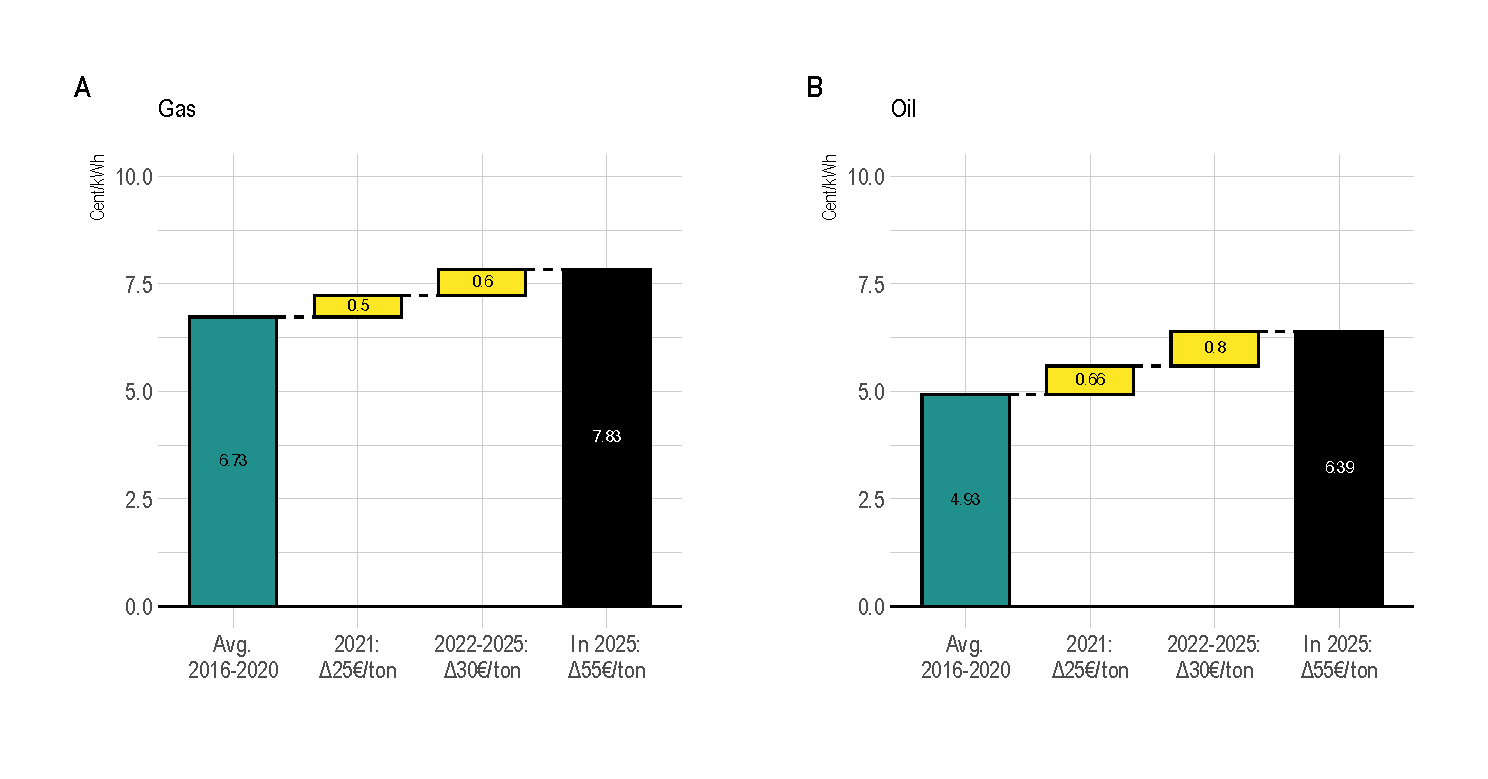
\includegraphics[width=1\linewidth]{figure/price_effect_behg} 

}

\caption[BEHG carbon price effects on gas and oil until 2025]{BEHG carbon price effects on gas and oil until 2025}\label{fig:behg}
\end{figure}
The relative price increases clearly show that considerable steering effects can already be expected from the BEHG in the next few years. Higher price levels driven by the structural price component of carbon pricing can be expected to have two impact channels. The first impact channel are short-term price reactions. Consumers adjust their demand levels for heating fuels due to higher prices (\protect\hyperlink{ref-alberini_etal11}{Alberini et al., 2011}). Short-term demand responses are of direct relevance when making predictions on the fuel demand of the buildings sector. The expected magnitude of the effect depends on the demand response, which is reflected in the short-term price elasticity of space heating demand.

The second impact channel is that structurally higher fossil fuel prices will create incentives for long-term investment in low-carbon heating technologies and energy efficiency. In the literature, long-term investment decisions driven by mitigation costs potentials are modeled using integrated assessment models (IAMs) for the buildings sector (e.g., \protect\hyperlink{ref-burger_etal19}{Bürger, Hesse, Köhler, Palzer, \& Engelmann, 2019}; \protect\hyperlink{ref-levesque_etal21}{Levesque et al., 2021}). Depending on the specific model structure, these IAM sector modules are often informed by assumptions on the price elasticities of heating demand as one of their input parameters.\footnote{For a more detailed example of how own price elasticities of demand are taken into account in IAMs, see the model structure description of the ETSAP TIAM model in \protect\hyperlink{ref-loulou_labriet08}{Loulou \& Labriet} (\protect\hyperlink{ref-loulou_labriet08}{2008}). Since IAMs vary in their specific structure and relations other models may consider price elasticities differently. Other very relevant parameters include the cost of capital and substitution elasticities.} Thus, empirical estimates of the price elasticity of space heating demand are also important for further analyses of the long-term steering effect with regard to investments in energy efficiency and low-carbon technologies in the buildings sector.

\textbf{Use of billing data as a complementary source of evidence}

Another line of argument for the relevance of this study is that the existing empirical evidence on the price elasticity of space heating demand is based on varying types of data sources, but to date few studies have been conducted based on energy billing data. For the case of Germany, ex-post statistical analyses for the residential buildings sector predominantly rely on panel data from social surveys (e.g., \protect\hyperlink{ref-rehdanz07}{Rehdanz, 2007}; \protect\hyperlink{ref-schmitz_madlener20}{Schmitz \& Madlener, 2020}; \protect\hyperlink{ref-schulte_heindl17}{Schulte \& Heindl, 2017}). The studies are build around the survey item \emph{household expenditure for heating}. But actual levels of energy demand and prices are not observed. This means that, for instance, different energy contract conditions between households may obscure real demand levels and thus affect the validity of the estimated results.

The data available for this thesis is different since the energy bills do provide both energy demand and associated costs on the level of the individual building. Previous studies based on energy billing data have, to the best of the authors' knowledge, only been conducted in the United States (see \protect\hyperlink{ref-auffhammer_rubin18}{Auffhammer \& Rubin, 2018}).

While the use of energy billing data offers unique characteristics that cannot be mirrored by social survey data, it should be pointed out that its use also has its weaknesses. Due to the data structure, the billing data does not observe demand responses at the level of an individual household but at the level of multi-apartment buildings. This creates an aggregation that may obscure the demand response of a single household. Furthermore, use of billing data makes the consideration of socio-economic determinants difficult (see Chapter \ref{conceptual-model}). In summary, it can thus be argued that the information value of estimates derived from billing data can be seen as complementary to the already existing estimates derived from social survey data.

Furthermore, the period under investigation in this thesis (2007-2019) is more recent than the period considered in other studies which adds to the relevance of this study.

\textbf{Research questions}

Given the recently tightened climate change mitigation targets for GHG emissions and the newly introduced carbon pricing for the buildings sector, additional evidence on price elasticities of space heating demand is of relevance. The aim of this work is therefore to produce own estimates of short-term price elasticities based on a large-scale energy billing sample in Germany. The guiding research questions for the analysis are:
\begin{itemize}
\tightlist
\item
  How does a change in energy price affect the level of space heating demand (price elasticity estimate)?
\item
  What other determinants do affect the level space heating demand and need to be considered so that their effects are not falsely attributed to energy prices?
\item
  And, are there any potential factors for heterogeneity in the sample that may not be reflected in the estimation of an overall mean price elasticity of demand?
\end{itemize}
To answer the above research questions, the thesis is divided into six Chapters. The first Chapter was used to provide an introduction, Chapter \ref{literature} provides a theoretical background on the price elasticity of demand and the prior literature to then develop a conceptual model for this thesis. In the following Chapter \ref{methods} the data and empirical approach are described. Furthermore, Chapter \ref{methods} also provides descriptive statistics on the empirical sample. Chapter \ref{results} provides the results of the statistical analysis. In Chapter \ref{discussion} the results are discussed. Chapter \ref{conclusion} provides concluding remarks.

\hypertarget{literature}{%
\chapter{Theory and Literature}\label{literature}}

The aim of this chapter is to provide the theoretical background on the price elasticity of demand and an overview of the previous literature on the price elasticity of space heating demand in particular. Subsequently, theory and evidence from the literature are used to develop a conceptual model with corresponding rationales for the relevance and expected direction of a variable's effect on space heating demand.

\hypertarget{theory}{%
\section{Price elasticity of demand}\label{theory}}

Elasticities, in general, are one of the key concepts in micro-economic theory. They are used to express the sensibility of one variable to a change in another. The own price elasticity of demand is one type of elasticity. It represents the magnitude of a change in demand of a good following from a change in its own price (\protect\hyperlink{ref-pindyck_rubinfeld18}{Pindyck \& Rubinfeld, 2018}). Formally, the own price elasticity of demand \(\epsilon\) can be expressed as:
\begin{equation}
\epsilon = \frac{\frac{\Delta Q}{Q}}{\frac{\Delta P}{P}} = \frac{P \Delta Q}{Q \Delta P}
\label{eq:ep}
\end{equation}
where \(\Delta P/P\) represents the percentage change in the own price \(P\) of a good and \(\Delta Q/Q\) the corresponding percentage change in the quantity \(Q\) demanded of the same good. Due to budget constraints, consumers tend to consume less of a good when its price increases, which implies that under normal conditions the price elasticity of demand is negative. But the responsiveness of the demand reaction may vary across different goods. A common conception in the econometric literature is that elasticities are a constant parameter (\protect\hyperlink{ref-varian10}{Varian, 2010}). Under the assumption of a constant price elasticity of demand, the associated demand function that can be expressed as:
\begin{equation}
Q = AP^{\varepsilon}
\label{eq:demand}
\end{equation}
where \(A\) represents an arbitrary constant and \(\epsilon\) again is the price elasticity of demand. Taking the logarithms of the demand function removes \(\epsilon\) from the exponent and yields:
\begin{equation}
ln(Q) = ln(A) + \epsilon \; ln(P)
\label{eq:demand2}
\end{equation}
which can be referred to as the elasticity case and will reappear at a later point in this thesis, when constructing the statistical regression models.

\textbf{The role of varying price elasticities of demand}

To make the underlying assumption of a constant elasticity more intuitive, it seems useful to return to the subject of interest for this thesis and show the behavior of demand curves for space heating under varying price elasticities of demand. Generally, the microeconomics literature distinguishes between three different \emph{types} of elasticities. If the demand response for a good is greater than the change in its own price (\(\epsilon < -1\)), the good is called to be price elastic. If the demand response is exactly equal to the change in price (\(\epsilon = -1\)), it is said to be unit-elastic. And if the demand response is smaller than the price change (\(0 > \epsilon > -1\)) -- indicating a lower price responsiveness -- it is said to be price inelastic (\protect\hyperlink{ref-pindyck_rubinfeld18}{Pindyck \& Rubinfeld, 2018}).\footnote{It should be noted that in the literature the minus of the demand elasticity \(\epsilon\) is sometimes omitted, as it is assumed that it is generally negative. However, I personally find it more intuitive not to do so -- especially when working empirically where positive estimates are a possibility -- and will therefore continue to use the negative values in this thesis.}
\begin{figure}

{\centering 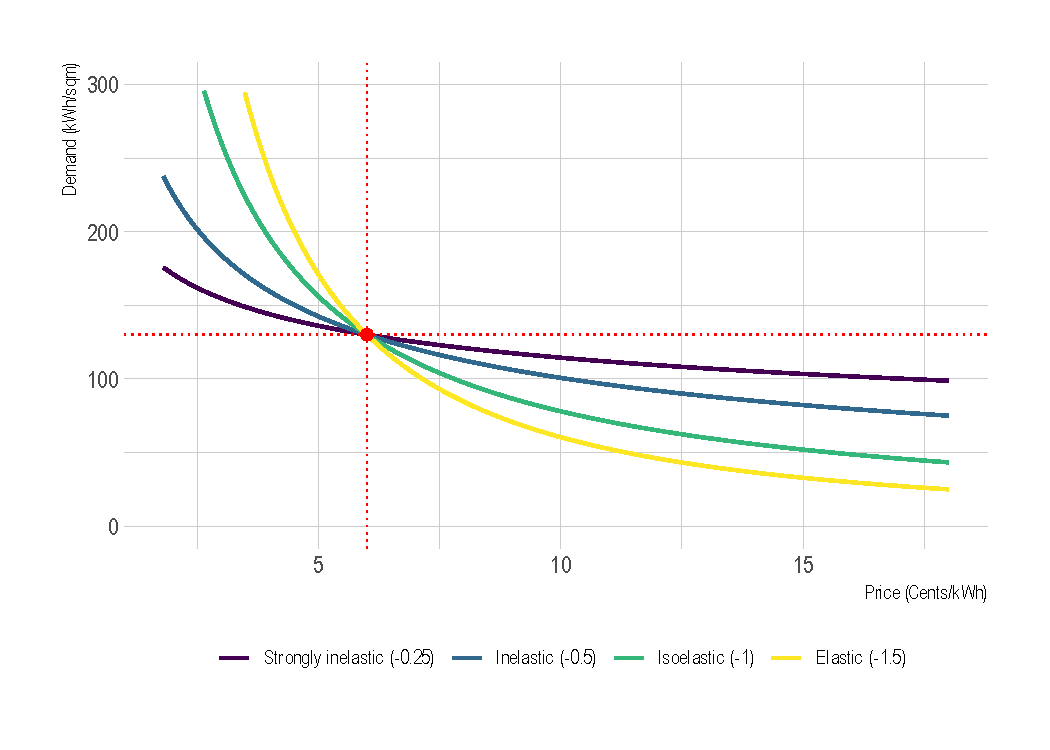
\includegraphics[width=1\linewidth]{figure/elasticities_plot} 

}

\caption{Exemplary demand curves associated with varying price elasticities of space heating demand}\label{fig:elasticities-conceptual}
\end{figure}
Figure \ref{fig:elasticities-conceptual} graphically represents demand curves for varying price elasticities of demand for space heating.\footnote{Please note that in the graph, energy price as the independent variable is plotted on the horizontal axis and energy demand as the response variable on the vertical axis. I consider this convention -- which is common in most of science -- to be more intuitive than the traditional Marshallian cross diagram in Economics, where the price is plotted on the vertical axis.} To construct the demand curves, a common arbitrary intersection point is chosen. The intersection point has a demand value of 130 kilowatt hours per square meter and year (kWh/sqm/y) and a price value of 6 Cents/kWh. These demand and price values are chosen because they reflect the average values in Germany for the period under investigation (see Chapter \ref{descriptives}). The graph includes a total of four demand curves with varying price elasticities: A unit-elastic (\(\epsilon = -1\)) demand curve, an elastic (\(\epsilon = -1.5\)) demand curve and two inelastic (\(\epsilon = -0.25, \epsilon = -0.5\)) demand curves.

The special feature of the unit-elastic demand curve (green) is that it gives the same result for total expenditure on heating costs for all combinations of price and demand. This is not the case with the other price elasticities. In the elastic case (yellow curve), total expenditures become lower when the price is higher, which means that households can adjust their demand downwards more. In the opposite, inelastic cases (purple and blue curves), on the other hand, households would reduce their demand less and therefore also face higher total expenditure. Conversely, to the left of the intersection point (lower prices), more elastic demand (yellow curve) leads to a higher level of energy demand and thus also to higher total expenditure than in the inelastic cases (purple and blue curves), where demand changes only gradually.

Different types of goods are structurally associated with different price elasticities of demand (\protect\hyperlink{ref-varian10}{Varian, 2010}). For the household demand for space heating it is reasonable to assume that demand will be is rather inelastic. There are two arguments that support this assumption. First, heating energy is to be regarded as an essential good that is associated with minimal demand in the winter months in order to ensure the well-being of residents. In general, essential goods tend to follow a more inelastic demand pattern than other types of goods (\protect\hyperlink{ref-gwartney76}{Gwartney, 1976}). Households can only reduce their space heating demand to a certain extent (right side of the intersection), but on the other hand, they do not have a strong rationality for a strong increase in heating demand beyond a comfortable level of warmth (left side of the intersection). The second indication for a rather inelastic demand is that especially tenant households, from which the data for this thesis originate, have only very limited to no practicable options to replace space heating from one source with space heating from another due to their dependence on the existing heating system. With limited ability to substitute comes the necessity for continued demand (\protect\hyperlink{ref-pindyck_rubinfeld18}{Pindyck \& Rubinfeld, 2018}).

\textbf{The difference between short- and long-term price elasticities of demand}

Another relevant dimension along which one distinguishes different price elasticities of demand is \emph{time}. More precisely, the time that elapses between a price signal and the measurement of the demand response. Here, the literature distinguishes between short-term and long-term price elasticities of demand (also called short- and long-run elasticities) (\protect\hyperlink{ref-pindyck_rubinfeld18}{Pindyck \& Rubinfeld, 2018}). Short-term elasticities of demand are those that are estimated in temporal proximity to the price change -- in this case, that would be the energy price change within a billing year and the associated change in demand in the same period. Long-term elasticities, on the other hand, imply that more time has elapsed for consumers to fully adjust to a price change and also to make long-term investment decisions that would change the overall level of demand (\protect\hyperlink{ref-pindyck_rubinfeld18}{Pindyck \& Rubinfeld, 2018}). For the subject at hand, such decisions may include changes in the isolation of a building or an exchange of the heating system. Long-term demand elasticities tend to be higher (more elastic) than their short-term counterparts (\protect\hyperlink{ref-schmitz_madlener20}{Schmitz \& Madlener, 2020}). Overall, the two types of short- and long term elasticities of demand can be seen as mirroring the two different channels through which a price-related policy instrument such as the BEHG can influence the demand behavior of residents (see Chapter \ref{relevance}).

In the literature, the approaches in the studies differ in the sense that they estimate either short-term and/or long-term price elasticities. For this thesis, I follow the example of \protect\hyperlink{ref-schmitz_madlener20}{Schmitz \& Madlener} (\protect\hyperlink{ref-schmitz_madlener20}{2020}) and only estimate short-term price elasticities of demand. Long-term price elasticities are often estimated using dynamic models, where the elasticity estimated between two periods represents a fraction of the long-term elasticity (e.g., \protect\hyperlink{ref-alberini_etal11}{Alberini et al., 2011}). However, since the methods vary more widely I consider it as outside of the scope of this thesis.

\hypertarget{review}{%
\section{Literature review}\label{review}}

In general, the study of the price elasticity of \emph{energy} demand is a broad field of academic research which also has a long history dating back to the mid-twentieth century (e.g., \protect\hyperlink{ref-cutler41}{Cutler, 1941}; \protect\hyperlink{ref-houthakker51}{Houthakker, 1951}). In the more recent past, as well a large number of academic studies have been published. These studies differ considerably in terms of focus and design. While a subset of studies focus on the demand responsiveness of private households for space heating in particular, most of the literature focuses on energy demand in general or other types of specific energy applications. To organize the comprehensive body of literature, I first focus on meta-studies to provide a first indication on price elasticity for energy in general, and then concentrate on the subset of relevant studies that focus on household space heating demand.

Several conceptual factors can systematically influence price elasticity estimates. The most important of these factors is the type of energy application analysed. The price responsiveness of private households for space heating demand is different form the price responsiveness for other types of energy application, such as the demand for transport fuels. Another relevant factor are different groups of consumers. Private households are likely to react differently to energy price changes than industrial or commercial consumers. Beyond those two dimensions, other factors which may also have an effect on elasticity estimates are the statistical methods used (time-series analysis, panel analysis, cross-sectional analysis), varying sources of data (national accounts, aggregate sector-level data, micro-data), varying spatial and temporal focus, measurement heterogeneity, and price trends (\protect\hyperlink{ref-csereklyei20}{Csereklyei, 2020}; \protect\hyperlink{ref-miller_alberini16}{Miller \& Alberini, 2016}).

\textbf{Meta-estimates as a first indication of price elasticity estimates}

To obtain a first indication of price elasticity estimates from previous studies, the meta-analysis by \protect\hyperlink{ref-labandeira_etal17}{Labandeira et al.} (\protect\hyperlink{ref-labandeira_etal17}{2017}) is particularly suitable. It covers a broad spectrum of energy applications and thus goes beyond previous meta-analyses that primarily focus on the elasticity of gasoline demand (e.g., \protect\hyperlink{ref-brons_etal08}{Brons, Nijkamp, Pels, \& Rietveld, 2008}; \protect\hyperlink{ref-havranek_etal12}{\textbf{havranek\_etal12?}}). Moreover, it is the most recent comprehensive meta-analysis and thus also partly covers the time period relevant for this thesis.

In their analysis, \protect\hyperlink{ref-labandeira_etal17}{Labandeira et al.} (\protect\hyperlink{ref-labandeira_etal17}{2017}) include a total of 428 papers, all published between 1990 and 2016. For the demand of natural gas, they find an average short-term (long-term) price elasticity of -0.18 (-0.57) based on 230 individual estimates. And for heating oil they find a comparable average short-term (long-term) elasticity of -0.19 (-0.54), which, however, is based on only 44 individual estimates (\protect\hyperlink{ref-labandeira_etal17}{Labandeira et al., 2017}). An average elasticity for space heating -- which is less focused on in the literature due to its relatively low prevalence -- is not provided.

The above average estimates of the price elasticity of demand for the energy carrier groups gas and oil are drawn from a wide range of consumer groups. This means that the underlying studies include not only those that examine demand response patterns for residential demand, but also others that examine these patterns for the commercial building stock and/or the industrial sector. \protect\hyperlink{ref-labandeira_etal17}{Labandeira et al.} (\protect\hyperlink{ref-labandeira_etal17}{2017}) also provide average price elasticities stratified by consumer groups, but these are, on the other hand, not clustered by the type of energy carrier. When differentiated along the dimension of consumer groups, they report that the average estimates are slightly higher in the residential household sector (short-term: -0.22; long-term: -0.62) than in the industrial sector (short-term: -0.17; long-term: -0.51), which seems reasonable given that households likely have more ability to change their level of demand than the industrial sector with more fixed production patterns and the ability to forward costs. Overall, however, the average price elasticity of demand estimates are all in a similar range and together convey the message that demand for energy is strongly inelastic in the short-term. This evidence is in line with the theoretical arguments that energy is an essential good and involves limited substitutability in many applications (see Chapter \ref{theory}).

The meta-estimates are useful in providing a high-level overview. However, as already mentioned, they include estimates from a wide range of energy applications that not necessarily reflect the demand response for the specific application of space heating in residential buildings. Furthermore, they are average estimates which may have the effect of masking discrepancies and variations between studies.

\textbf{Subset of studies focusing on the price elasticity of space heating demand in the residential buildings sector}

The studies focusing on space heating demand of the residential sector represent a subset of the stream of literature estimating price elasticities of energy demand. The subset of individual studies presented in the following were selected based on the twin criteria that they make specific estimates for the energy application of space heating in the residential buildings sector and are of good quality (only peer-reviewed journal articles). An overview of the selected studies is provided in Table \ref{tab:estimates-literature}.

There are three earlier studies that have a spatial focus on Germany. The first study was conducted by \protect\hyperlink{ref-rehdanz07}{Rehdanz} (\protect\hyperlink{ref-rehdanz07}{2007}), who estimates short-term price elasticities for different energy carrier groups for residential space heating demand. She uses social survey data on household-level heating expenditures from the Socio-Economic Panel (SOEP) in the years 1998 and 2003. Methodologically, a cross-sectional statistical analysis with dummy variables is conducted for the two years. In contrast to the meta-estimates presented in the previous part of the Chapter, the study finds that demand for heating oil is highly elastic with estimates ranging between -1.68 and -2.03, depending on the model specification. For gas, the results indicate an inelastic elastic demand between -0.44 and -0.63 (depending on the model specification) which is nevertheless significantly more elastic than the meta-estimates presented previously. Therefore, the study concludes that the type of energy carrier can have a strong influence on the price sensitivity of private households (\protect\hyperlink{ref-rehdanz07}{Rehdanz, 2007}).
\begin{table}[]
\centering
\caption{Selected studies on the price elasticity of space heating demand}
\label{tab:estimates-literature}
\resizebox{\textwidth}{!}{%
\begin{tabular}{@{}llll@{}}
\toprule
\textbf{Study} & \textbf{Type of data used} & \textbf{\begin{tabular}[c]{@{}l@{}}Energy \\ carrier\end{tabular}} & \textbf{\begin{tabular}[c]{@{}l@{}}Short-term\\ price elasticities\end{tabular}} \\ \midrule
 &  &  &  \\
{\ul \textit{Studies with spatial focus on Germany}} &  &  &  \\
\multirow{2}{*}{Rehdanz (2007)} & \multirow{2}{*}{\begin{tabular}[c]{@{}l@{}}Social survey, cross-sectional data (SOEP),\\ all types of buildings, 1998 and 2003\end{tabular}} & Gas & -0.44 to -0.63 \\
 &  & Oil & -1.68 to -2.03 \\
Schmitz and Madlener (2020) & \begin{tabular}[c]{@{}l@{}}Social survey, panel data (SOEP), \\ all types of buildings, 1996-2014\end{tabular} & (All) & -0.31 to -0.43 \\
Schulte and Heindl (2017) & \begin{tabular}[c]{@{}l@{}}Social survey, panel data (EVS),\\ all types of buildings, 1993-2008\end{tabular} & (All) & -0.50 \\
 &  &  &  \\
{\ul \textit{Studies with focus on other countries and regions}} &  &  &  \\
Alberini et al. (2011) & \begin{tabular}[c]{@{}l@{}}US, household-level social survey, \\ 50 metropolitan areas, panel data, 1995-2007,\\ only single-family homes and duplexes\end{tabular} & Gas & -0.57 to −0.69 \\
Auffhammer and Rubin (2018) & \begin{tabular}[c]{@{}l@{}}US, energy billing data, household-level, \\ only California, panel data, 2003-2014\end{tabular} & Gas & -0.17 to -0.23 \\
\begin{tabular}[c]{@{}l@{}}Leth-Petersen and \\ Togeby (2001)\end{tabular} & \begin{tabular}[c]{@{}l@{}}Denmark, apartment-block level (\textgreater{}1,500 sqm),\\ panel data, 1984-1995\end{tabular} & Oil & -0.08 \\
 &  & District heating & -0.02 \\
\multirow{2}{*}{Meier and Rehdanz (2010)} & \multirow{2}{*}{\begin{tabular}[c]{@{}l@{}}UK, household-level social survey,\\ panel data 1991-2005\end{tabular}} & Gas & -0.34 to -0.56 \\
 &  & Oil & -0.40 to -0.49 \\
Metcalf and Hassett (1999) & \begin{tabular}[c]{@{}l@{}}US, household-level, panel data, \\ 1984, 1987 and 1990\end{tabular} & Gas & -0.48 to -0.71 \\ \bottomrule
\end{tabular}%
}
\end{table}
In a more recent study, as well based on the SOEP social survey data but covering a more comprehensive time period between 1996 and 2014, \protect\hyperlink{ref-schmitz_madlener20}{Schmitz \& Madlener} (\protect\hyperlink{ref-schmitz_madlener20}{2020}) find a price elasticity of space heating and hot water demand of -0.31 to -0.43, depending on the model specifications. They do not differentiate the elasticities by energy carrier group. The price elasticities are derived from household expenditure elasticities, as demand is not directly observed in the SOEP social survey data. In contrast to \protect\hyperlink{ref-rehdanz07}{Rehdanz} (\protect\hyperlink{ref-rehdanz07}{2007}), the study uses a panel structure where observations are clustered by households and years using fixed-effects regression models. They produce much lower price elasticity estimates, which are more consistent with the meta-estimates presented previously. Moreover, the study discovers that price elasticity is heterogeneous across different socio-economic groups. Given the household-level information at their disposal, they find that higher-income households are less sensitive to energy price changes than lower-income households. Likewise, homeowners show less sensitivity than tenant households (\protect\hyperlink{ref-schmitz_madlener20}{Schmitz \& Madlener, 2020}).

Also with a focus on Germany, \protect\hyperlink{ref-schulte_heindl17}{Schulte \& Heindl} (\protect\hyperlink{ref-schulte_heindl17}{2017}) investigate the price and expenditure elasticities of private energy demand in Germany between 1993 and 2008. For their analysis, they use survey data from the \emph{Einkommens- und Verbrauchsstichprobe (EVS)} and analyse them with a demand system approach. More precisely, they estimate a quadratic expenditure system. For space heating demand, they find an own price elasticity of -0.50 across all households. They further observe that the price elasticity changes with the level of total household expenditure, with households in higher expenditure strata reacting more strongly to price changes (\protect\hyperlink{ref-schulte_heindl17}{Schulte \& Heindl, 2017}). Put differently, this means that following an increase in price level low income households tend to lower energy demand to a lesser extent as compared to households with a higher income. Thus, regarding the effect of household income, their results are contradictory to those of \protect\hyperlink{ref-schmitz_madlener20}{Schmitz \& Madlener} (\protect\hyperlink{ref-schmitz_madlener20}{2020}).

Besides the studies focusing on Germany, Table \ref{tab:estimates-literature} also reports the findings from five other international studies. \protect\hyperlink{ref-alberini_etal11}{Alberini et al.} (\protect\hyperlink{ref-alberini_etal11}{2011}) examine household demand for gas (and electricity) in single-family homes and duplexes using household-level social survey data in 50 metropolitan areas in the United States (US) over the period 1995-2007. As a modelling approach, they use static (short-term elasticities) and dynamic (long-term elasticities) panel models. For the static models, reflecting the approach also taken in this thesis, they find an own price elasticity of private gas demand between -0.57 and -0.69, depending on the model specification. These estimates are in their magnitude comparable to the results of an earlier study by \protect\hyperlink{ref-metcalf_hassett99}{Metcalf \& Hassett} (\protect\hyperlink{ref-metcalf_hassett99}{1999}) who use the 1984, 1987 and 1990 waves of the US Residential Energy Consumption Survey (RECS) to examine homeowners' investments in energy efficiency measures and as part of their study find price elasticities of residential gas demand range between −0.48 and −0.71.

In contrast to these estimates, a recent study done by \protect\hyperlink{ref-auffhammer_rubin18}{Auffhammer \& Rubin} (\protect\hyperlink{ref-auffhammer_rubin18}{2018}) finds that the short-term price elasticity of residential gas demand is even more inelastic. Instead of covering the whole US the study focuses on California in particular. The estimates for the price elasticity of gas demand range between -0.17 and -0.23. The study by \protect\hyperlink{ref-auffhammer_rubin18}{Auffhammer \& Rubin} (\protect\hyperlink{ref-auffhammer_rubin18}{2018}) is especially interesting because it is the only previous study that also relies on data from energy bills. The data analysed covers the period 2003-2014 and consists of monthly energy bills at the household-level. Although the data is similar in principle, there are two structural differences with the energy bills used in this thesis. First, gas tariffs in the US can change monthly rather than annually. Thus, the dataset includes more frequent observations, but may also suffer from more simultaneity of price and demand due to less regulation of the market in the US. Furthermore, another difference is that the data from \protect\hyperlink{ref-auffhammer_rubin18}{Auffhammer \& Rubin} (\protect\hyperlink{ref-auffhammer_rubin18}{2018}) corresponds to individual households and not to the aggregate building-level.

In addition, the study by \protect\hyperlink{ref-leth-petersen_togeby01}{Leth-Petersen \& Togeby} (\protect\hyperlink{ref-leth-petersen_togeby01}{2001}) provides evidence from Denmark. They rely on a panel data approach and analyse data from 1984-1995 on apartment buildings with a floor area of more than 1,500 square meters. Similar to this study they also use the building-level as the level of analysis. As an empirical strategy, they rely on fixed effects models and find highly inelastic demand responses for space heating. For oil, the short-term price elasticity is found to be -0.08 and for district heating -0.02, meaning almost no demand response to a changing price at all.

Another study by \protect\hyperlink{ref-meier_rehdanz10}{Meier \& Rehdanz} (\protect\hyperlink{ref-meier_rehdanz10}{2010}) focuses on the United Kingdom (UK) and analyses a household-level social survey panel for the 15-year period 1991-2005. For their model they use a log-linear approach. They find that the short-term price elasticity of demand for gas ranges from -0.34 to -0.56, depending on the specification. For residential oil demand, the results are in the same order of magnitude, but narrower, between -0.40 and -0.49. In addition, they find that the type of occupant is a relevant dimension for a different price responsiveness. While renters show a higher responsiveness to price changes, homeowners showed a more inelastic demand response.

\textbf{Synthesis of price elasticity estimates from the literature}

When summarizing the literature on the price elasticity of residential space heating demand presented previously, commonalities and differences emerge. The most important commonality is that the price elasticity of energy demand in general and household space heating demand in particular is inelastic in almost all empirical estimations. However, there are differences in the magnitude of the estimates between the individual studies. While the meta-results by \protect\hyperlink{ref-labandeira_etal17}{Labandeira et al.} (\protect\hyperlink{ref-labandeira_etal17}{2017}) as well as a number of individual studies indicate a strongly inelastic demand response (e.g. \protect\hyperlink{ref-auffhammer_rubin18}{Auffhammer \& Rubin, 2018}; \protect\hyperlink{ref-leth-petersen_togeby01}{Leth-Petersen \& Togeby, 2001}), other individual studies still indicate an inelastic but higher demand response (e.g., \protect\hyperlink{ref-alberini_etal11}{Alberini et al., 2011}; \protect\hyperlink{ref-meier_rehdanz10}{Meier \& Rehdanz, 2010}; \protect\hyperlink{ref-metcalf_hassett99}{Metcalf \& Hassett, 1999}; \protect\hyperlink{ref-rehdanz07}{Rehdanz, 2007}; \protect\hyperlink{ref-schmitz_madlener20}{Schmitz \& Madlener, 2020}; \protect\hyperlink{ref-schulte_heindl17}{Schulte \& Heindl, 2017}). These differences in magnitude may be partly due to the different local and temporal conditions of the studies or due to differences in the data and methodology.
\begin{figure}

{\centering 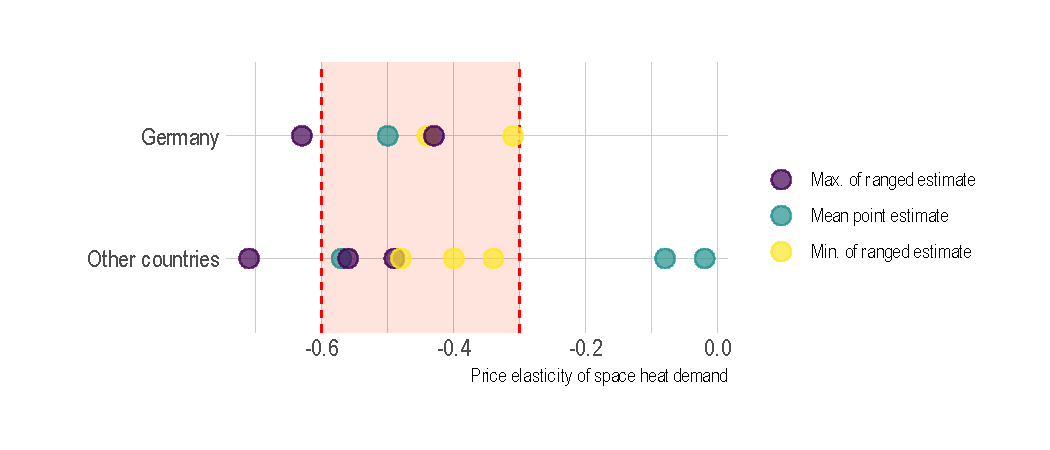
\includegraphics[width=1\linewidth]{figure/plot_literature_estimates} 

}

\caption{Price elasticity estimates for space heat demand from individual studies}\label{fig:literature-estimates-plot}
\end{figure}
Figure \ref{fig:literature-estimates-plot} graphically summarizes the short-term elasticity estimates from the individual studies on space heating demand. All studies that focused on Germany found somewhat more responsive price elasticities ranging between -0.3 and -0.6.\footnote{Note that the extreme results of \protect\hyperlink{ref-rehdanz07}{Rehdanz} (\protect\hyperlink{ref-rehdanz07}{2007}) for oil as the carrier type are omitted here. They rely on a cross-sectional regression analysis with only two isolated time periods considered. Therefore, the estimates must be considered more prone to extreme results than is the case with a longer panel.} And also the majority of estimates from other countries or regions is reflected by that range for the price elasticity.

Another common feature that links all the individual studies presented is that they do not focus on one-off extreme price shocks as an identification strategy, but on gradual price developments. They are mostly built around a panel data set covering a longer period of time. The period examined in this study also covers more than a decade with rather gradual price developments. This should therefore be considered an important condition that facilitates the comparability of the results of this study with the estimates presented in the literature.

\hypertarget{conceptual-model}{%
\section{Conceptual model}\label{conceptual-model}}

The previous two parts of the Chapter presented the theoretical foundations on the price elasticity of demand (see chapter \ref{theory}) and the previous evidence from the literature on household demand response for space heating to energy price changes (see chapter \ref{review}). To synthesize this basis, this final part of the Chapter is dedicated to developing a conceptual model relying on both theory and approaches from previous studies. The aim is to identify relevant determinants for the level of space heating demand of private households and to justify their relevance. The conceptual model will then be transferred into a statistical model and empirically examined in the further course of this thesis.

\textbf{Price elasticity of demand}

The starting point for the development of the conceptual model is the relationship between energy price and space heating demand, the assumption from the theory of price and demand being that the demand for space heating is influenced by the changes in the energy price. If the energy price goes up, energy demand moves down along the demand curve and vice versa (see Figure \ref{fig:elasticities-conceptual}). Expressed in a statistical terminology, this implies that space heat demand is the response variable of a model and energy price the main explanatory variable. In order to support the development of the conceptual model visually, Figure \ref{fig:dag} depicts it as a directed acyclic graph (DAG). At the center of the DAG, the response variable space heat demand (yellow bubble) is shown, the variance of which is to be explained. The effect of energy price (purple bubble) on space heating demand represents the \emph{price elasticity of demand} and is therefore highlighted by the red arrow.
\begin{figure}

{\centering 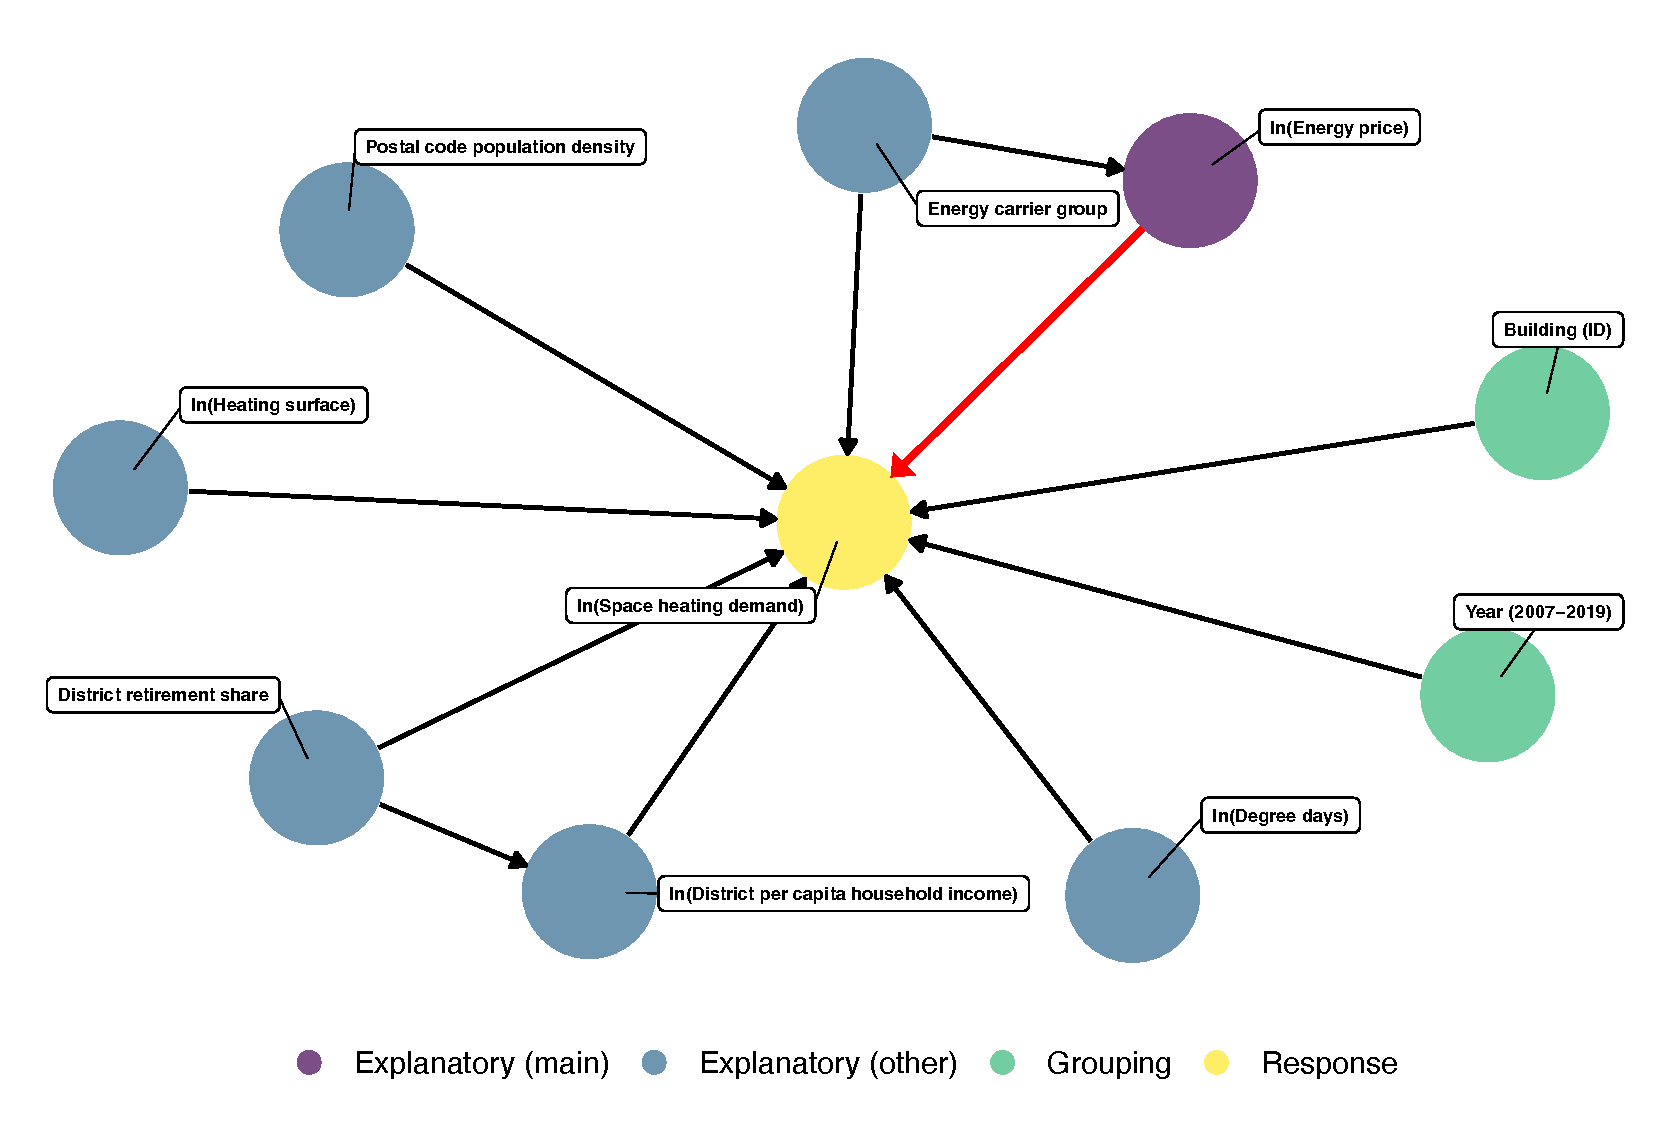
\includegraphics[width=1\linewidth]{figure/dag_red} 

}

\caption[Conceptual model as directed acyclic graph]{Conceptual model as directed acyclic graph}\label{fig:dag}
\end{figure}
In addition to energy price, there are an array of other determinants that may influence the level of space heating demand. These are shown in the DAG as additional explanatory variables (blue bubbles) and as grouping variables (green bubbles). To determine the set of additional relevant variables, a structured approach was used. First, the recent study by \protect\hyperlink{ref-schmitz_madlener20}{Schmitz \& Madlener} (\protect\hyperlink{ref-schmitz_madlener20}{2020}) was considered as a suitable starting point to create a list of variables. Second, the other individual studies presented previously (see Chapter \ref{review}) were then used to cross-validate the initial list of variables as well as to screen for further ones. This structured approach led to the variables presented and reasoned for in the following.

\textbf{Climatic conditions}

First, the consideration of the local climatic conditions in a billing period is of importance, as they can have a strong effect on space heating demand (\protect\hyperlink{ref-hesse20}{Heße, 2020}). Due to the high relevance of climatic conditions, all individual studies presented in Chapter \ref{review} consider and control for them. For the practical implementation, climatic conditions are usually approximated by the outdoor temperature over a defined period of time and aggregated to periodical (heating) degree days. The basic intuition for the influence of varying climatic conditions is that with lower outdoor temperatures, transmission heat losses increase and thus the demand for space heating increases to compensate for indoor heat losses. In line with \protect\hyperlink{ref-vdi13}{VDI} (\protect\hyperlink{ref-vdi13}{2013}), degree days in this study are defined as the temperature difference between a room temperature of 20°C and the daily average outdoor temperature, provided it is below a heating limit of 15°C.\footnote{It should be noted that the definition of degree days used here differs from the internationally frequently used definition of heating degree days (HDD), which is calculated by difference between the average outdoor temperature below a heating threshold over time -- regardless of an additionally defined room temperature. In this thesis, the VDI based definition of \emph{degree days} was chosen, as this is the common methodology in Germany. It is, for example, also used to create a comparable scoring for building energy performance certificates (see \protect\hyperlink{ref-halbig_namyslo14}{Halbig \& Namyslo} (\protect\hyperlink{ref-halbig_namyslo14}{2014})).} Lower mean outdoor temperatures are associated with a higher aggregated number of degree days in a period. Consequently, as a rationale for the direction of the effect of degree days, one would expect a higher space heating demand when degree days are higher in an annual heating period and vice versa. Varying degree days occur on a temporal (one period is warmer/cooler than another) and on a spatial scale (places at higher altitudes or in the interior of the continent have structurally lower temperatures).

\textbf{Building-level characteristics}

In addition, two building-level characteristics are included in the model as additional explanatory variables. First, the size of a building can influence the heat demand, as in larger buildings the ratio between the external surface of the building and the heating surface decreases. Thus, the relative share of transmission heat losses per unit of heating surface is lower correspondingly. Following this rationale, it must be assumed that in buildings with a larger heating surface -- which approximates the size of a building -- the space heating demand per unit is lower if all other factors are to remain constant.

Second, the type of energy carrier used for the heating system is another building-level characteristic, which is considered in almost all previous studies (see Chapter \ref{review}). The intuition for the inclusion of the energy carrier as a categorical control variable (oil, gas, district heating) is that different types of energy carriers are associated with different heating technologies, which may lead to structural differences in energy use and efficiency. This effect may also be further amplified by the fact that certain energy carriers have been more commonly introduced in certain time periods in the past. This means that, for example, an average oil heating system may be older and thus less energy efficient than an average gas heating system due to technological progress.

\textbf{District socio-economic variables}

Besides building-related characteristics, socio-economic variables may also affect the level of space heating demand. In the literature that draws its data from social surveys, household-level socio-economic information such as income, number of inhabitants, age, education level or employment status is usually part of the core survey data and therefore considered as control variables in the analysis (e.g., \protect\hyperlink{ref-meier_rehdanz10}{Meier \& Rehdanz, 2010}; \protect\hyperlink{ref-rehdanz07}{Rehdanz, 2007}; \protect\hyperlink{ref-schmitz_madlener20}{Schmitz \& Madlener, 2020}). This study, in contrast, relies on energy billing data at the building-level, which can provide a more accurate picture of actual energy demand and prices than social surveys, but in return does not provide socio-economic information, neither at the household nor at the aggregated building-level. However, as previous studies provide good arguments that the inclusion of socio-economic variables is relevant, an attempt is made to account for their relevance by using the most accurate data available at the district or postal code level. The approach here is that even if they cannot capture household-level effects, they might nonetheless capture overlapping socio-economic effects at a higher level of aggregation.

The first of the three socio-economic variables included is the per capita household income at the district-level. In line with most of the literature, one would expect lower income to lead to lower heating demand as households have fewer funds at their disposal. However, it could also be that income at the district level is more of an approximation of the general affluence of a district and therefore effects such as lower economic resources available for investment in building efficiency outweigh the budget perspective, possibly leading to an opposite outcome. Secondly, retirement share is considered as an additional socio-economic variable at the district-level. Here, the intuition is that with high retirement rates in a district more people spend more of their time at home which may lead to a rise in space heat demand. Lastly, the population density within a postal code area is considered to observe if there may be structural differences in heating demand between densely populated metropolitan areas on the one hand and sparsely populated rural areas on the other.

\hypertarget{methods}{%
\chapter{Methods}\label{methods}}

\hypertarget{data}{%
\section{Data description and pre-processing}\label{data}}

To translate the conceptual model set up in Chapter \ref{conceptual-model} into a statistical model that can be used to empirically investigate the price elasticity of space heating demand, data from multiple sources were combined.

\textbf{Energy billing dataset}

The key dataset is a large-scale building-level panel of energy bills made available though the Climate Policy Department at DIW Berlin. The data originates from the energy- and billing service provider ista Deutschland GmbH and was provided for scientific use.\footnote{Due to the sensitivity of the data, it is to be classified as confidential. Access was exclusively via DIW Berlin's internal servers. Due to data protection regulations, it is not possible to make the data available to external parties for the purpose of reproducing the results.} The sample contains information on an average of multi-unit residential buildings in Germany and ranges from 2007 to 2019.\footnote{The While the demand data is available from the start, energy prices are first observed in 2007. Thus, the time period analysed ranges from 2007 to 2019.} The smallest buildings observed have two living units; single-family houses with just one unit are not observed. The observations in the dataset represent annual heating bills at the building-level. The dataset contains the two main variables for the analysis: space heating demand and energy price. It also contains additional building-level information including the heating surface, the number of housing units, the type of energy carrier used for heating. The dataset also provides a building-level ID and the billing dates suitable to create a panel structure.

\textbf{Space heat demand (kWh/sqm/a):} The demand data in the billing dataset is provided as total energy consumed per building and per annual billing period in kilowatt hours (kWh). To isolate the share of energy consumed for the purpose of space heating, the share of energy used for hot water production is deduced for those buildings where hot water production is also done via the central heating system. In a second step, in order to obtain a comparable metric for the differently sized buildings in the sample, the total space heating demand at building level is divided by the building heating surface in square meters (sqm). This results in the annual space heat demand per square meter as the demand variable. For a summary of the variables and their data sources see Table \ref{tab:variables}.

\textbf{Energy prices (Cents/kWh):} The structure of the price data in the dataset is similar to that of the demand data. The energy price data is provided as total annual costs at the building-level in Euros. Again, relying on the supplementary information on the relative shares of energy use for space heating and hot water generation in buildings where hot water is provided via the central heating system, the cost share for space heating alone is identified. In a second step, the cost share for space heating is then translated into average per-unit costs by dividing total costs for space heating by the respective demand for space heating in kWh. To make the cost scale more intuitive, prices are furthermore converted from Euros to Cents. This yields a per-unit energy price variable (Cents/kWh). Additionally, since energy prices are provided as nominal prices, they are deflated using the German annual consumer price index (CPI) with 2015 as the index year (\protect\hyperlink{ref-destatis21}{DESTATIS, 2021b}). The use of the CPI to deflate energy prices represents the standard procedure in the literature, which is also used by \protect\hyperlink{ref-schmitz_madlener20}{Schmitz \& Madlener} (\protect\hyperlink{ref-schmitz_madlener20}{2020}), for example.

Energy contracts for private households in Germany usually consist of a fixed cost component (flat-rate basic charge) and a variable cost component (consumption-based price per kWh).\footnote{On the basis of exemplary heating bills provided by ista, it was possible to determine that this was also the case for the data in the billing sample.} The data does not contain a breakdown of fixed and variable costs, but only the total costs, which are then converted into average costs per-unit (the sum of fixed and variable costs divided by the quantity demanded) as described in the previous paragraph. There is much debate in the literature about whether the household demand response to changes in energy prices depends on the average price or instead on the marginal price. The use of marginal prices would be necessary if the variable price component were to change based on the quantity consumed (``block pricing'') and could also be dynamically adjusted by the utility, as is the case for many private household contracts in the USA, for example (see \protect\hyperlink{ref-auffhammer_rubin18}{Auffhammer \& Rubin, 2018}). Since those factors do not apply for the energy contracts underlying the billing data used in this thesis, I assume the use of the average per-unit energy price to be suitable, as it was also done in other studies (e.g., \protect\hyperlink{ref-metcalf_hassett99}{Metcalf \& Hassett, 1999}; \protect\hyperlink{ref-rehdanz07}{Rehdanz, 2007}; \protect\hyperlink{ref-schmitz_madlener20}{Schmitz \& Madlener, 2020})

Another problem is whether the demand decisions depend on the price in the same period or on the price of the previous period, so that the calculation of the previous period influences the current demand decisions. Following the approach of \protect\hyperlink{ref-schmitz_madlener20}{Schmitz \& Madlener} (\protect\hyperlink{ref-schmitz_madlener20}{2020}), I generally construct the model with the price in the same period. However, to check the robustness of the results, I also run models with the price of the previous period.

\textbf{(Billing) Year:} The billing data contains the exact dates of the billing period of an individual building. While most billing periods mirror the calendar year, some buildings have billing periods occurring during the year. Therefore, the start and end dates of the billing periods are used to make an allocation to billing years. For billing periods during the year, the allocation is based on which of the two calendar years contains the majority of days in the billing period.

\textbf{Energy carrier group:} There are three main types of energy carriers included in the dataset: Gas, oil, and district heating. To obtain these three categories, energy carrier descriptions from the dataset are grouped under these categories (e.g, \emph{Gas low} and \emph{Gas high} are grouped under \emph{Gas}). In addition, all other heating carriers which have only limited occurrence in the sample (e.g.~electricity for heat pumps, coal combustion) are grouped under the category \emph{Others} and later excluded from the analysis due to the relatively small number of observations and heterogeneity of carrier types within the group (see Chapter \ref{workflow}).

\textbf{Heating surface (sqm):} Information on the heating surface of a building is given in square meters at building-level. The heating surface does not correspond to the total floor area of a building, as it excludes the unheated surfaces within a buildings (e.g., building corridors or basements). Heating area was chosen over the number of housing units as an alternative approximation for the size of a building. The reasons for this are that it was assumed that the heating surface better reflects the ratio between the interior and exterior area of a building since it does not suffer from varying sizes of housing units.\footnote{While this paper uses building heating surface as a continuous variable, other studies with a less detailed database often use building size categories, which can be seen as a similar approach.}
\begin{table}[]
\centering
\caption{Variables and data sources}
\label{tab:variables}
\resizebox{\textwidth}{!}{%
\begin{tabular}{@{}lllll@{}}
\toprule
\textbf{Variable} & \textbf{} & \textbf{Type} & \textbf{Unit} & \textbf{Data source} \\ \midrule
 &  &  &  &  \\
\textit{\begin{tabular}[c]{@{}l@{}}Demand\\ \end{tabular}} & Space heat demand & Continuous & ln(kWh/sqm/a) & Ista (billing data) \\
\textit{} &  &  &  &  \\
\textit{\begin{tabular}[c]{@{}l@{}}Price\\ \end{tabular}} & Energy price & Continuous & ln(Cents/kWh) & Ista (billing data)\\
\textit{} &  &  &  &  \\
\multirow{4}{*}{\textit{\begin{tabular}[c]{@{}l@{}}Additional billing \\information\\ \end{tabular}}} & Heating surface & Continuous & ln(sqm) & Ista (billing data)\\
 & Energy carrier group & Categorical & Gas / Oil / District heating & Ista (billing data)\\
 & Building ID & Categorical & - & Ista (billing data)\\
 & Year & Categorical & - & Ista (billing data)\\
\textit{} &  &  &  &  \\
\textit{\begin{tabular}[c]{@{}l@{}}Climatic conditions\\ \end{tabular}} & Degree days & Continuous & ln(degree days) & IWU (2021) \\
\textit{} &  &  &  &  \\
\multirow{3}{*}{\textit{\begin{tabular}[c]{@{}l@{}}Socio-economic factors\\ \end{tabular}}} &  District per capita household income & Continuous & ln(Euros/a) & Statistische Ämter (2021) \\
 & District retirement share & Continuous & \% & DESTATIS (2021a) \\
 & Postal code population density & Continuous & ln(inhabitants/sq. km) & OSM (2021), OSM (2021a) \\ \bottomrule
\end{tabular}%
}
\end{table}
\newline

\textbf{Supplementary data sources}

\textbf{Degree days:} Degree days were retrieved from an Excel tool compiled by the \emph{Institut für Wohnen und Umwelt (IWU)} at the postal code level (\protect\hyperlink{ref-iwu21}{IWU, 2021}). The degree days data from the IWU-tool builds on daily temperature data from the 800 weather stations of the German Meteorological Service (DWD) that are aggregated on a monthly basis. In the tool, the settings of a mean room temperature of 20°C and a heating limit of 15°C are chosen to reflect the VDI based definition of degree days (\protect\hyperlink{ref-vdi13}{VDI, 2013}). Furthermore, the option to assign the postal code area to the three nearest DWD weather stations with weighting according to geographical distance is chosen. This is because relying on reduce the risk of possible distortions due to differences in altitude between a single weather station and the centroid of a postal code area. The extracted monthly degree day figures per postal code area are then aggregated to annual periods on a rolling basis and matched with the annual building-level energy billing observations. The postal code level was chosen because it corresponds to the spatial information on the location of the buildings contained in the billing data and therefore represents the most accurate allocation possible.

\textbf{District per capita household income (Euros/a):} As a district-level income variable to approximate for varying incomes, the per capita disposable income of private households provided by the joint statistical portal of the federal and state governments is used (\protect\hyperlink{ref-statistischeamter21}{Statistische Ämter, 2021}). The figure includes the primary income of private households, minus transfers paid and plus transfers received. Disposable income is chosen because it can be considered the most suitable indicator for funds available for households. The district-level is chosen as it is the most granular household income statistics available.

\textbf{District retirement share (\%):} To construct the district retirement share variable, population data at the district-level with a segmentation by age groups is used (\protect\hyperlink{ref-destatis21c}{DESTATIS, 2021a}). As an approximation for the actual proportion of retirees, the percentage of persons within a district and year who are 65 years of age and older is calculated. This approach was chosen because no detailed statistics are available on the number of people in retirement at the district-level. The boundary value of 65 was chosen as the age group closest to the current retirement age in Germany and since the same threshold was also chosen in the literature (e.g., \protect\hyperlink{ref-alberini_etal11}{Alberini et al.} (\protect\hyperlink{ref-alberini_etal11}{2011}))

\textbf{(Postal code) Population density (inh./sq. km):} To generate the population density variable, data from Open Street Maps with pre-assigned population figures to postal code areas based on the 2011 Census were used (\protect\hyperlink{ref-osm21}{OSM, 2021b}, \protect\hyperlink{ref-osm21a}{2021a}). The postal code level and not the district level was chosen because, firstly, a higher granularity of data was available and, secondly, the use of districts as the level of analysis may obscure heterogeneity within districts. Especially when they are rural districts with a city. To determine the population density variable, the number of inhabitants per postal code was divided by the base area in square kilometers (sq. km), giving the population density as the average number of inhabitants per sq. km.

\hypertarget{empirical-model}{%
\section{Empirical approach}\label{empirical-model}}

\textbf{Causality with observational data}

The conceptual DAG presented in Chapter \ref{conceptual-model} and the derived rationales for the cause-and-effect relationships between space heat demand and energy price in an environment where the other explanatory variables also exert an effect on energy demand are all based on the assumption of causal inference. Causal inference can be described as indicating that an observed relationship between two variables is reflected by a causal link and not just mere correlation (\protect\hyperlink{ref-holland86}{Holland, 1986}). The analysis in this thesis is build on externally provided observational data. Using observational data to draw causal inference about a treatment effect -- in the given case, inference about the price sensitivity of private households for space heating demand in multi-family buildings in Germany -- is inherently difficult since the treatment is not controllable and therefore cannot be randomly assigned (\protect\hyperlink{ref-nichols07}{Nichols, 2007}). Since an experimental research design, which would arguably provide the most unbiased source of evidence, is not feasible for this research, it is all the more important to point out potential sources of bias in the estimation process relying on observational data and address those biases where possible.

\textbf{Potential sources of bias}

Reducing potential sources of bias was approached in several steps. First, the set of explanatory variables already described was used to reduce potential bias from omitted variables. This means that by taking into account, for example, degree days or the heating surface of a building, additional relevant effects on the level of heating demand are captured that might otherwise be wrongly attributed to the role of energy price alone.

On the other hand, there is also an additional gap in the data in relation to the omitted variables that cannot be fully remedied. Due to the aggregated nature of the data at the building-level, it is not possible to integrate detailed household-level socio-economic variables (e.g., household income, number of inhabitants, age, education level, or employment status) into the analysis. In other studies which build on household-level social surveys socio-economic variables have been found to be a relevant determinant of energy demand -- especially household income is a variable that has been found to exert a relevant effect (e.g., \protect\hyperlink{ref-meier_rehdanz10}{Meier \& Rehdanz, 2010}; \protect\hyperlink{ref-rehdanz07}{Rehdanz, 2007}; \protect\hyperlink{ref-schmitz_madlener20}{Schmitz \& Madlener, 2020}). To at least partially address the fact that socio-economic variables are not available at the household level, socio-economic controls at the district or postcode level are used to try to capture the underlying socio-economic effects at a higher level.

Another source of potential bias can result from data errors. In general, the use of observational data should not be considered a mechanistic process, but should be based on the application of domain-specific knowledge to critically evaluate and challenge the available data. In view of the potentially distorting effects of data errors, the use of domain-specific knowledge and expert judgement was important in cleaning and processing the energy billing dataset. The process is described in detail later in this Chapter (see Chapter \ref{Workflow}). When evaluating the energy price variable, outliers are found that can be traced back to be placeholders that do not reflect the actual energy demand. If these observations had not been removed from the analysis, they would have distorted the result of the analysis.

In addition, it was checked if the measurement of the variables incorporated any systematic measurement error and concluded that a systematic error was not present. Generally, several variables used in the analysis might be subject to measurement error. For example, the degree days data are based on a spatial interpolation of the values from the three nearest DWD weather stations to the centroid of a postal code, which introduces a first layer of measurement error. It is then assumed that the degree days assigned to a postal code apply to every building within that postal code, even though there may be greater distances and differences in elevation between the centroid and the building's location representing a second layer . However, errors such as those described exemplarily for the degree days variable do not necessarily represent a problem, since a systematic deviation is required for the existence of a systematic error (bias). Rather, the described exemplary derivations from a true value for outdoor temperature indicate a random inaccuracy in the measurement of the variable, which is less serious in general and especially given the very large number of observations in the sample. The same logic applies, for example, to the construction of the energy demand variable. While aggregation at the building level introduces some inaccuracy compared to a hypothetical measurements at the household-level, it does not lead to a systematic error.

\textbf{Simultaneity problem}

Furthermore, when estimating price elasticities of demand, one additional relevant challenge for the identification of a causal effect is the potential simultaneous determination of price and demand leading to a market equilibrium
\begin{itemize}
\item
  Use of multiple estimation techniques (panel regression, Bayesian mutilevel models)
\item
  Issue of Simultaneity (See Aufhammer)
\item
  If demand is assumed to depend on the marginal block price, then price and consumption are simultaneously determined, and instrumental variable estimation techniques must be used (Burtless and Hausman, 1978; McFadden et al., 1978; Wilder and Willenborg, 1975; Hewitt and Hanemann, 1995; Reiss and White, 2005). For lack of exact information about the block rates faced by the consumers, however, we are forced to use average price.
\item
  Perhaps most importantly, research on the elasticity of demand for natural gas must also consider multiple potential sources of endogeneity. The first source of endogeneity is the classic simultaneity that stems from the fact that quantity and price result from the equilibrium in a system of equations. Unlike the electricity sector, for natural-gas customers' rates change on a monthly basis---updating as a function of gas wholesale prices paid by the retail utilities.
\item
  From Aufhammer wegen IV approach: We instrument the utilities' consumer-facing prices with the weekly average spot price of natural gas at a major natural gas distribution hub in Louisiana (the Henry Hub). This instrument is valid, as we know the formula of how utilities pass-through the price (providing a strong first stage), and the price is determined prior to within-bill consumption (strengthening the exclusion restriction).
\end{itemize}
\textbf{Frequentist estimation approach}

For the analysis, I use several statistical methods. For the full sample analysis, I rely on Frequentist estimation approaches given the large number of data points in the billing dataset. For the subsequent analysis of a stratified random subsample I rely on Bayesian methods. Generally, I follow a logic where I begin with constructing a simple model specification and then extend it to a more elaborate statistical model. The goal partly being to be able to compare model estimates by varying methods and predictors included.

To start with, I formulate the statistical model for the full sample analysis as a simple cross-sectional multiple linear regression (MLR) model based on ordinary least squares (OLS) (\protect\hyperlink{ref-bailey17}{Bailey, 2017}; \protect\hyperlink{ref-wooldridge13}{Wooldridge, 2013}):
\begin{align*}
ln(Demand) & = \alpha + \beta_1 \cdot ln(Price) + \beta_2 \cdot ln(Degree.days) + \\
 & \quad \beta_3 \cdot ln(Heating.surface) + \beta_{4} \cdot Carrier.group.oil + \\
 & \quad \beta_{5} \cdot Carrier.group.district.heating + \beta_{6} \cdot ln(District.income) + \\
 & \quad \beta_{7} \cdot District.retire + \beta_{8} \cdot ln(Pop.density) + \varepsilon 
\end{align*}
where the response variable \(ln(Demand)\) denotes the natural logarithm of the annual space heating demand per square meter, the main explanatory variable \(ln(Price)\) denotes the natural logarithm of the average energy price (Cents/kWh) in the same period. The other terms of the linear equation denote the additional explanatory variables (degree days, building characteristics, and district/postal code socio-economic variables) and \(\varepsilon\) denotes the error term of the model. Referring back to equation \eqref{eq:demand2} from the theory Chapter, the ln-form of both sides of the equation transforms the model into the elasticity case. Therefore, the coefficient \(\beta_1\) of \(ln(Price)\) represents the price elasticity of space heating demand. For the cross-sectional OLS regression, I first run the model with \(ln(Price)\) as a sole predictor and then with the additional explanatory variables included.

In the billing dataset, there is both a building ID, which allows observations from several periods to be assigned to the same building, and information on the billing period. Thus, the data allows to go beyond cross-sectional OLS and apply panel data estimation techniques. In the OLS estimation shown above, observations from various buildings and years are treated to be systematically no different from each other. Panel data methods, on the contrary, are rooted in the assumption that there may be systematic and unobserved differences between units that may be correlated with observed predictors whose effects on the response are to be measured (\protect\hyperlink{ref-wooldridge13}{Wooldridge, 2013}). Thus, panel data methods are considered a powerful tool for observational data where controlling for all relevant factors is inherently difficult (\protect\hyperlink{ref-bailey17}{Bailey, 2017}). By acknowledging and addressing that there may be unobserved inter-individual differences between the units (buildings) and also an intra-individual dynamic over time (years), use of panel data methods can provide a more accurate picture for the predictors observed in the model.

For the subject at hand, it is likely that the demand for space heating observed is impacted by various unobserved building-specific constant or semi-constant factors, such as a building's energetic condition or its usage properties. Thus, inferences drawn from cross-sectional data are likely to be invalid since building-specific fixed-effects are falsely attributed the observed model predictors -- including energy price. The same applies for temporal trends. For example, new buildings with higher energetic standards could be added to the sample over the course of the period under investigation and old buildings might drop out of the sample due to demolition. Such factors, which affect the structural composition of the sample over time, may result in space heating demand in the later periods being systematically lower than that in the earlier periods. In the empirical literature, switching from a cross-sectional model to the use of unit-level fixed effects with panel data resulted in a more inelastic estimates for the price elasticity of space heating demand (\protect\hyperlink{ref-miller_alberini16}{Miller \& Alberini, 2016}).

In addition, the choice of panel estimation method should provide more reliable results even when strict exogeneity fails to hold. Therefore, I adopt a two-way fixed effects (FE) model, which is considered one of the more robust estimation methods and is also a commonly used approach in the prior literature on the price elasticity of heating demand (\protect\hyperlink{ref-lange_etal14}{Lange, Moro, \& Traynor, 2014}; e.g., \protect\hyperlink{ref-meier_rehdanz10}{Meier \& Rehdanz, 2010}; \protect\hyperlink{ref-schmitz_madlener20}{Schmitz \& Madlener, 2020}). The FE model takes the following form:
\begin{align*}
ln(Demand_{i,t}) & = \alpha + \beta_1 \cdot ln(Price_{i,t}) + \beta_2 \cdot ln(Degree.days_{i,t}) + \\
 & \quad \beta_3 \cdot ln(Heating.surface_{i,t}) + \beta_{4} \cdot Carrier.group.oil_{i,t} + \\
 & \quad \beta_{5} \cdot Carrier.group.district.heating_{i,t} + \beta_{6} \cdot ln(District.income_{i,t}) + \\
 & \quad \beta_{7} \cdot District.retire_{i,t} + \beta_{8} \cdot ln(Pop.density_{i,t}) + \\
 & \quad \gamma_{building[i]} + \delta_{year[t]} + \varepsilon_{i,t}
\end{align*}
The FE model structure extends the cross-sectional OLS model. The response variable \(ln(Demand_{i,t})\) again denotes the natural logarithm of the annual space heating demand per square meter but extended by the indices on building \(i\) and the annual time period \(t\). The same applies to \(ln(Price_{i,t})\) as the average energy price (Cents/kWh) and the set of additional explanatory variables. The newly added term \(\gamma_{building[i]}\) denotes the time-invariant building fixed-effects and \(\delta_{year[t]}\) the annual time fixed-effects. \(\varepsilon_{i,t}\) again denotes the error term.

In line with the approach for the OLS cross-sectional model, I first run the model without the additional explanatory variables to obtain an estimate for the case where only the energy price is used to explain demand, and then include the set of additional explanatory variables in a second specification. Additionally, for the FE model, I also drop variables with limited explanatory power to arrive at a more condensed and relevant model specification. Furthermore, I also run a model where \(ln(Price_{i,t)}\) is substituted by \(ln(Price_{i,t-1})\), so taking the lag of the price variable in \(t-1\) instead of the price in the same period to explain the space heating demand in period \(t\).

All the models described represent the conditional demand. It therefore has to be inferred that the results reflect the short-term price elasticities of demand. The use of other dynamic estimation approaches to estimate long-term elasticities, as for example \protect\hyperlink{ref-alberini_etal11}{Alberini et al.} (\protect\hyperlink{ref-alberini_etal11}{2011}) or \protect\hyperlink{ref-csereklyei20}{Csereklyei} (\protect\hyperlink{ref-csereklyei20}{2020}) have done, would go beyond the scope of this thesis and are therefore not pursued. Additionally, the short-term price elasticities estimated here may also be viewed as lower bound estimates of the price responsiveness compared to the usually higher long-term estimates. As they are a lower bound estimate, they can also be considered as a conservative estimate for any kind of modelling or policy advice for which they might be used.

To estimate the OLS models, I rely on the lm-function in R. To estimate the FE models, I used the felm-function from the lfe-package (\protect\hyperlink{ref-gaure2013lfe}{Gaure, 2013}).

\textbf{Bayesian estimation approach}

Beyond the use of OLS and FE as \emph{classical} Frequentist methods used on the full sample, I move to the use of Bayesian inference when further analyzing a stratified random subsample of the data. In general, use of Bayesian inference has the advantage of allowing for the propagation of uncertainty in the modelling process (\protect\hyperlink{ref-mcelreath20}{McElreath, 2020}). Furthermore, the Bayesian framework allows for a more intuitive interpretation of modelling results being the actual chance of an event happening rather than the probability that the same outcome would occur if one were to replicate the data (\protect\hyperlink{ref-mcelreath20}{McElreath, 2020}). A further advantage of Bayesian inference on application where data is scarce would also be that due to the logic of updating beliefs based on evidence (data), integration of prior knowledge is possible (\protect\hyperlink{ref-gelman_etal21}{Gelman, Hill, \& Vehtari, 2021}). Here, I refrain from making strong assumptions on the prior distribution of model parameters and instead rely on weakly informed priors. Additionally, it should be pointed out that Bayesian inference is more computationally demanding than the methods presented above -- especially when integrating a model with a multilevel structure. This is the reason why Bayesian inference is only used on a subsample and not for the analysis of the full sample.

The subsample is set up a stratified random selection of 400 buildings per energy carrier group from the full sample. In In delimitation to the full sample analysis, the subsample analysis intends to serve two purposes. First, as mentioned in the previous paragraph, use of fewer data points makes the application of Bayesian methods possible which are well-suited to propagate uncertainty. Second, potential sources of heterogeneity in the price responsiveness shall be investigated. The stratified sampling approach where all three energy carrier groups are represented equally, allows the investigation of the carrier type as an potential additional source of heterogeneity. Furthermore, having a stronger representation of district heating than in the main sample also allows for a glimpse into the near future, when more gas and oil heating will become unviable due to the gas energy crisis and rising carbon prices, and will therefore be replaced by district heating (or heat pumps).\footnote{Heat pumps are not considered here due to the still very limited data available on heat pump use in the billing sample.}

For the analysis of the subsample, I first run the simple models that mirror the specifications from the OLS but in a Bayesian setting. When moving to the FE models I resort to the use of a multilevel partial pooling model with varying intercepts (\protect\hyperlink{ref-mcelreath20}{McElreath, 2020}). In the FE model, where information is clustered by the same units (buildings and years), there is no information sharing between units. This may lead to less reliable especially for the buildings cluster where there are sometimes only a few observations for one building. The multilevel partial pooling model with varying intercepts for each building and annual period, on the other hand, allows for information sharing among groups when estimating those intercepts (\protect\hyperlink{ref-mcelreath20}{McElreath, 2020}). For Together with the weakly informed priors mentioned earlier, the main model with the multilevel structure therefore takes the following form:
\begin{align*}
ln(Demand_{i,t}) & \sim \operatorname{Normal}(\mu_{i,t}, \sigma) \\
\mu_{i,t} & \sim \bar\alpha + \gamma_{building[i]} + \delta_{year[t]} + \beta_1 \cdot ln(Price_{i,t}) +  \\
 & \quad \beta_{2} \cdot ln(Degree.days_{i,t}) + \beta_{3} \cdot ln(Heating.surface_{i,t}) + \\
 & \quad \beta_{4} \cdot Carrier.group.oil_{i,t} + \beta_{5} \cdot Carrier.group.district.heating_{i,t} + \\
 & \quad \beta_{6} \cdot ln(District.income_{i,t}) + \beta_{7} \cdot District.retire_{i,t} + \beta_{8} \cdot ln(Pop.density_{i,t}) \\
\bar\alpha & \sim \operatorname{Normal}(0, 1) \\
\gamma_j & \sim \operatorname{Normal}(0, \sigma_{\gamma}) \\
\delta_k & \sim \operatorname{Normal}(0, \sigma_{\delta}) \\
\beta_{1-8} & \sim \operatorname{Normal}(0, 0.5) \\
\sigma, \sigma_{\gamma}, \sigma_{\delta} & \sim \operatorname{Exponential}(1)
\end{align*}
Also for the Bayesian models, the response variable \(ln(Demand_{i,t})\) denotes the natural logarithm of the annual space heating demand per square meter in building \(i\) in the year \(t\) and the main explanatory variable \(ln(Price_{i,t})\) denotes the natural logarithm of the average energy price (Cents/kWh) in the same period. The intercept term (\(\bar \alpha\)) denotes the varying intercepts along the two grouping variables for partial pooling building (\(\gamma_{building[i]}\)) and year (\(\delta_{year[t]}\)). For the model I assume that all parameters follow a Gaussian distribution centered on 0. The intercept term \(\bar \alpha\) is assumed to have a standard deviation of 1. The distribution parameter \(\sigma\) as well as the parameters \(\sigma_{\gamma}\) and \(\sigma_{\delta}\) for the varying intercepts parameters were assumed to follow an \(Exp(1)\) distribution so that they are limited to the positive values required for the standard deviation.

In the subsample analysis it is further the goal
\begin{align*}
ln(Demand_{i,t}) & \sim \operatorname{Normal}(\mu_{i,t}, \sigma) \\
\mu_{i,t} & \sim \bar\alpha + \gamma_{building[i]} + \delta_{year[t]} + \beta_1 \cdot ln(Price_{i,t}) +  \\
 & \quad \beta_{2} \cdot ln(Degree.days_{i,t}) + \beta_{3} \cdot ln(Heating.surface_{i,t}) + \\
 & \quad \beta_{4} \cdot Carrier.group.oil_{i,t} + \beta_{5} \cdot Carrier.group.district.heating_{i,t} + \\
 & \quad \beta_{6} \cdot ln(District.income_{i,t}) + \beta_{7} \cdot District.retire_{i,t} + \beta_{8} \cdot ln(Pop.density_{i,t}) + \\
 & \quad \beta_{9} \cdot ln(Price_{i,t}) \cdot Carrier.group.oil_{i,t} + \\
 & \quad \beta_{10} \cdot ln(Price_{i,t}) \cdot Carrier.group.district.heating_{i,t} \\
\bar\alpha & \sim \operatorname{Normal}(0, 1) \\
\gamma_j & \sim \operatorname{Normal}(0, \sigma_{\gamma}) \\
\delta_k & \sim \operatorname{Normal}(0, \sigma_{\delta}) \\
\beta_{1-10} & \sim \operatorname{Normal}(0, 0.5) \\
\sigma, \sigma_{\gamma}, \sigma_{\delta} & \sim \operatorname{Exponential}(1)
\end{align*}
The second model is an extension to the previous model introducing an additional interaction term between main explanatory variable \(ln(Price_{i,t})\) and the categorical variable energy carrier group. Gas serves as the reference category.

The Bayesian models are estimated using the brms-package by \protect\hyperlink{ref-burkner17}{Bürkner} (\protect\hyperlink{ref-burkner17}{2017}) in R. The brms-package serves as an interface to the probabilistic programming language and interence engine Stan (\protect\hyperlink{ref-standevelopmentteam22}{Stan Development Team, 2022}).
\begin{itemize}
\tightlist
\item
  \url{https://cu-psych-computing.github.io/cu-psych-comp-tutorial/tutorials/r-extra/brms/multilevel-models-with-brms/}
\end{itemize}
All from Labanderira et al.

discrete decision to purchase durable goods that consume energy and the decision to consume energy is rarely considered.renovations may disturbe the picture the panel data provides

On the other hand, most empirical studies in this area have used single-equation econometric models that require separability restrictions. This is a severe disadvantage as it is not possible to estimate cross-price effects between different energy products or consider the effects of non-energy products on the price elasticity of energy goods.

Sample period. It is widely accepted that the economic cycle has a strong influence on energy consumption due to income and (indirect cycle-related) price effects. In the case of economic crises, for example, a depression of energy prices may occur; reduced disposable income may lead agents to reduce consumption through improvements in energy efficiency, adjustments to other types of consumption or changes towards other more inexpensive energy goods.

\hypertarget{workflow}{%
\section{Workflow}\label{workflow}}

In Figure \ref{fig:workflow1} the first part of the workflow of the empirical analysis is depicted. The upper part describes the data processing and the merging of the data. The bottom part shows the regression analyses performed on the full sample using ordinary least squares (OLS) and fixed effects (FE) regressions.

In Figure \ref{fig:workflow2} the second part of the workflow is shown. After using Frequentist estimation techniques on the full sample, the analysis moves to the application of Bayesian regression analysis. For this purpose, a stratified random subsample by energy carrier group is created including 400 buildings per energy carrier group (Gas, Oil, District heating). Additionally, the subsample is used to investigate potential factors of heterogeneity in price responsiveness in the data first resorting to exploitative visual analysis and then moving to construct an interaction term model.

\textbf{Processing of billing sample and matching with supplementary data}

The energy billing data requires several steps of data processing to clean the data, which are shown in the upper part of Figure \ref{fig:workflow1}. After the data cleaning, 2,719,270 of the original 4,494,943 annual billing observations (60.5\%) remain for the full sample analysis. The criteria applied in the cleaning process are ordered by the number of observations removed.
\begin{figure}

{\centering 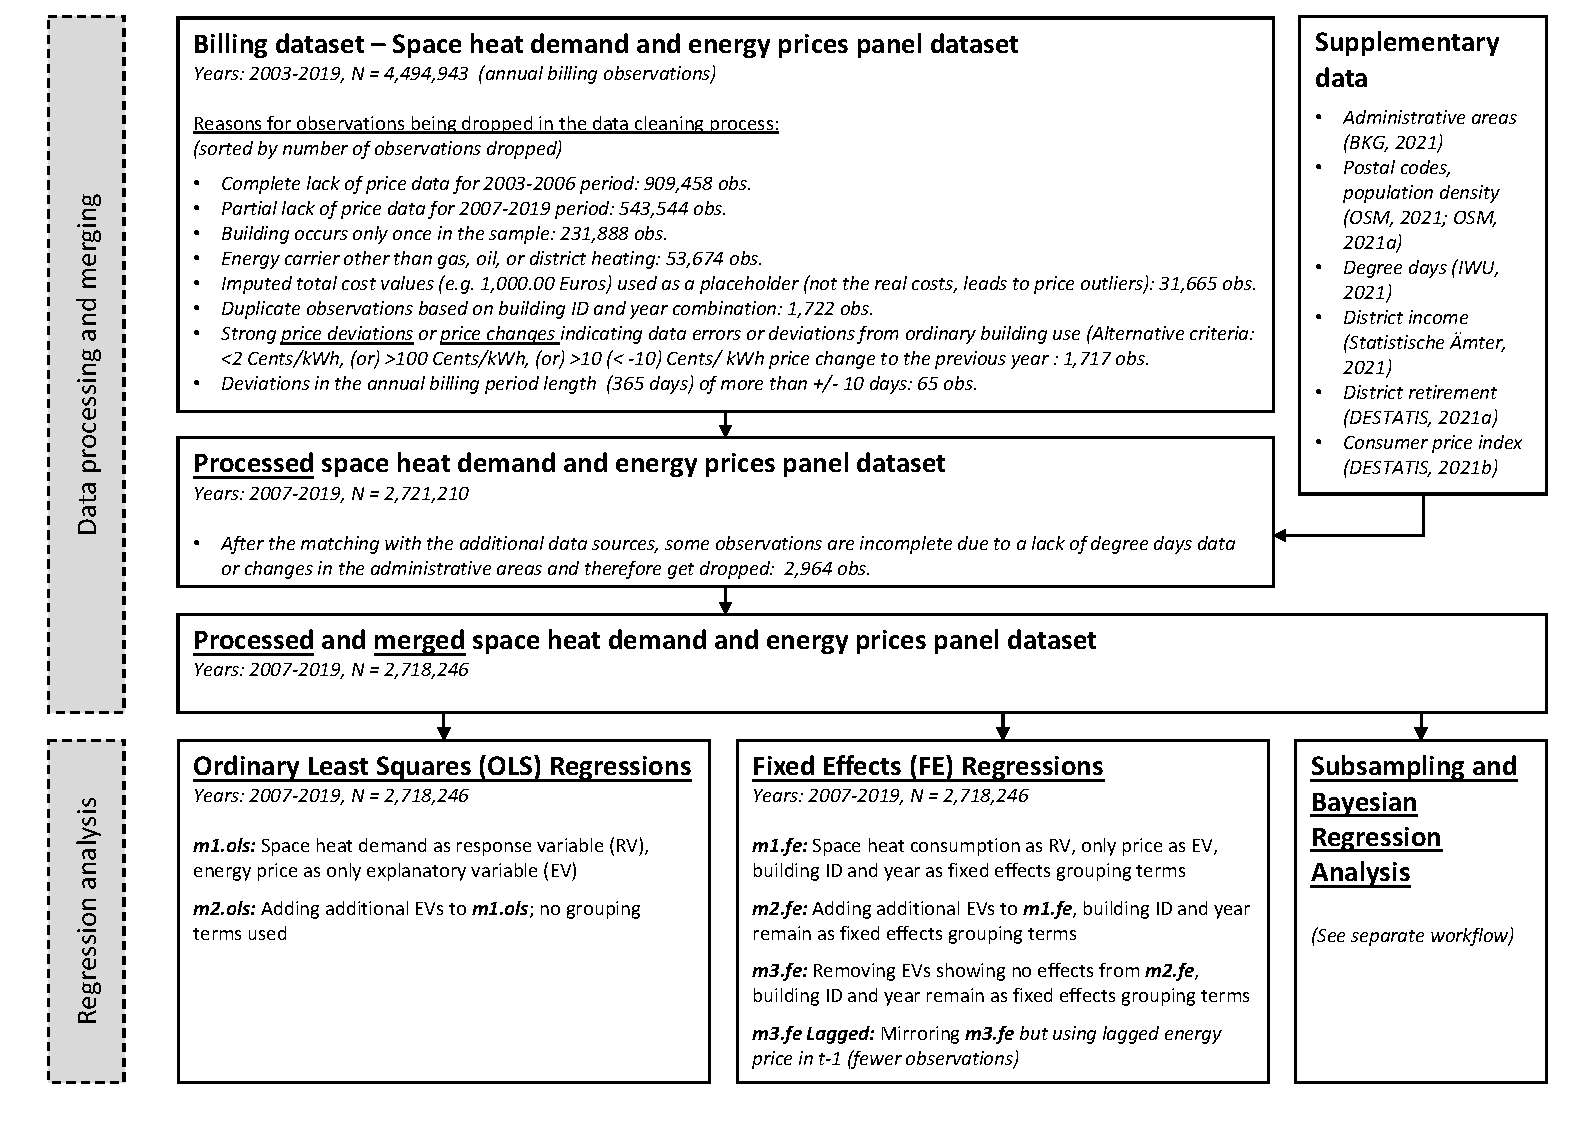
\includegraphics[width=1.03\linewidth]{figure/workflow_diagramm_part1} 

}

\caption{Workflow of data processing and regression analysis based on full sample}\label{fig:workflow1}
\end{figure}
The most important reason for exclusion from the sample is the absence of price data. In the period 2003-2006, price data are not available for any of the observations. This leads to the exclusion of 909,458 observations. In addition, price data are also missing for a part of the observations in the period 2009-2019. Due to these gaps in the price data, a further 543,544 observations are excluded from the dataset. A further 233,888 observations are removed from the sample because they are associated with buildings that occur only once in the sample. The decision to apply this criterion was mainly due to the fact that singular building IDs occurred mainly in the period 2007-2008, suggesting that IDs from this period are not linked with observations in later periods. Furthermore, observing a building at least twice during the analysed period allowed for cross-validation of matching building attributes and therefore better reliability of the data. Another 53,674 observations were removed from the sample because the buildings are heated with an energy carrier other than gas, oil, or district heating. Due to the small number of buildings compared to the total sample size and due to the heterogeneity of the group (both very modern buildings with heat pumps and un-renovated buildings with coal heating), it was decided to exclude all other energy carriers from the sample. In addition, another 1,722 observations were excluded as duplicates (matching building ID and year) and 65 observations due to a deviating length of the billing period (deviation of more than +/- 10 days).

In addition to the factors described above, there are two other reasons for excluding observations from the sample. Both reasons are related to outliers in the energy price data. Compared to the other cleaning steps described above, performing the analysis with and without these two steps in place has shown that they can have a strong effect on the results of the analysis and are therefore particularly important.

First, it was determined through exploratory testing and confirmed by ista that the price data contains fictitious cost values (e.g., 1,000.00 Euros for the entire building) that are used as placeholders and do not reflect actual costs. These fictitious cost values arise because ista, as a billing service provider, does not always have information about the costs incurred by the building owners and therefore uses the placeholders for internal technical reasons. The actual costs are only entered later by the building owners and therefore do not appear in the sample.\footnote{The internal practice of ista was reconstructed on the basis of an email exchange for the Wärmemonitor 2019, in which it was confirmed that the price data contain fictitious cost values.} This practice leads to the formation of outliers in the energy price data, as the fictitious cost values do not necessarily reflect the size and characteristics of a building. A total of 31,665 observations are removed due to fictitious cost values identified by searching for round cost rates without cent amounts that occur unusually often in the sample.

Second, despite the removal of the fictitious cost values, some spurious outliers remained in the price data. An exploratory review of individual cases revealed that the remaining price outliers were likely due to data errors (e.g., unrealistic heating areas), which is not unusual given the very large number of observations in the sample. Although a relatively small number, the price outliers can significantly interfere with the results of the analysis. Therefore, it was decided to also exclude the remaining observations that showed unrealistic deviations from the reasonable price level expected during the time period under investigation (real prices: \textless2 cents/kWh or \textgreater100 cents/kWh) or large price changes from one period to another (real prices: \textgreater10 or \textless-10 cents/kWh compared to the previous year). The exclusion thresholds were based on expert judgments and were chosen to exclude only highly of implausible observations. Use of the thresholds resulted in the exclusion of an additional 1,717 observations from the sample.

The processed billing data are then matched with the external data sources (see figure \ref{fig:workflow1}). Due to missing degree days data or changes in the administrative areas, a further 1,940 observations are removed from the sample here, which ultimately leads to 2,719,270 remaining observations. After the processing, these observations are both complete and systematically checked for data errors that may have affected the outcome of the analysis.

\textbf{Regression analysis based on full sample}

{[}STILL MISSING{]}

\textbf{Stratified subsampling and Bayesian regression analysis}

{[}STILL MISSING{]}
\begin{figure}

{\centering 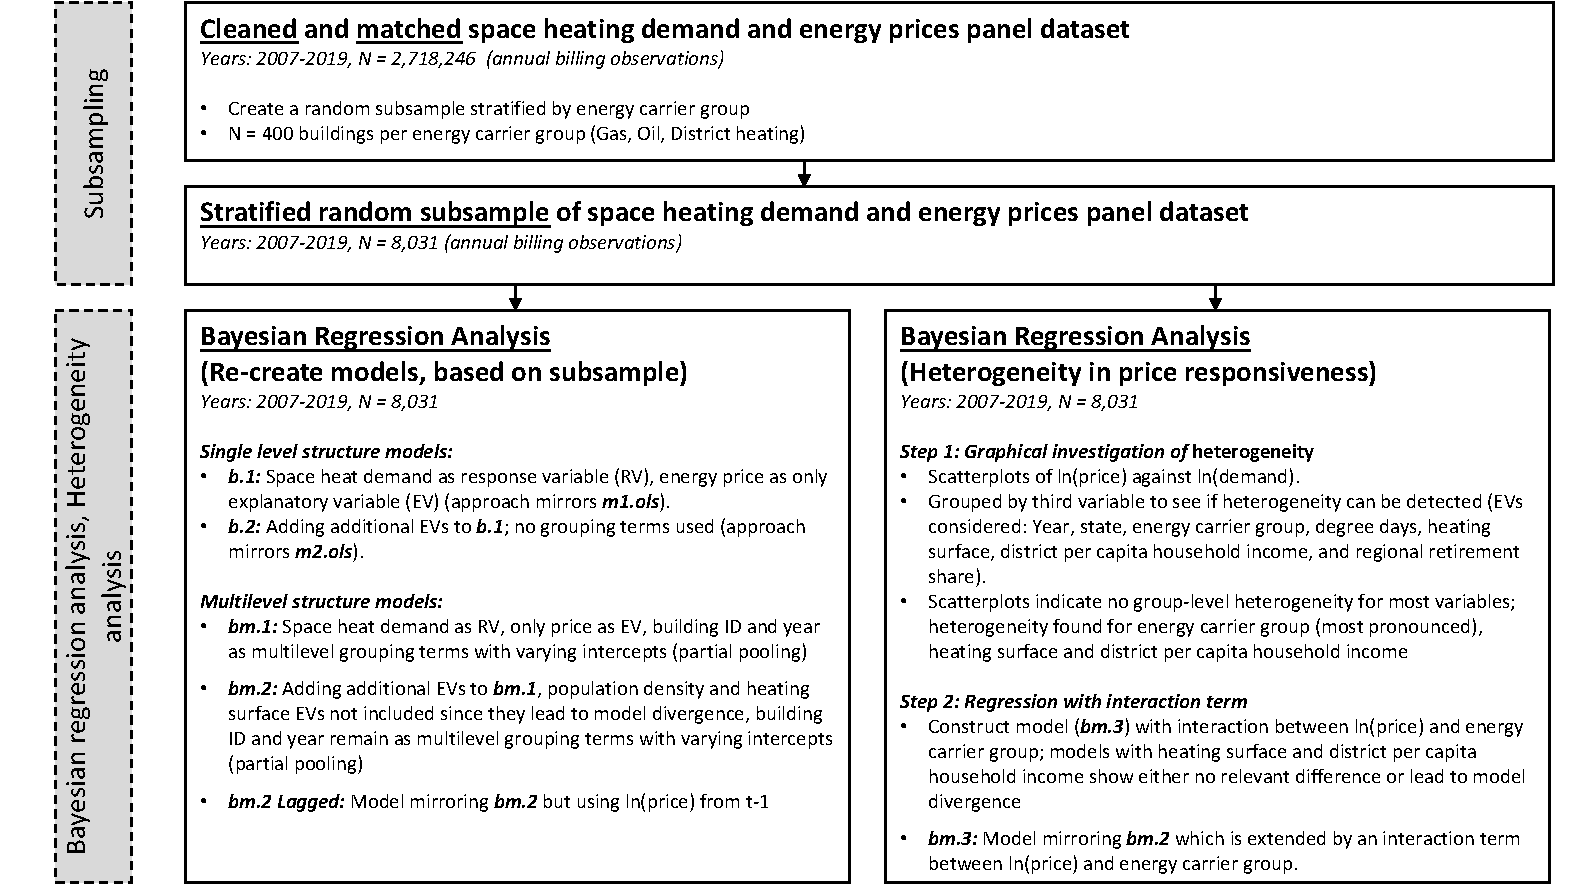
\includegraphics[width=1.03\linewidth]{figure/workflow_diagramm_part2} 

}

\caption{Workflow of stratified subsampling and Bayesian regression analysis based on subsample}\label{fig:workflow2}
\end{figure}
\hypertarget{descriptives}{%
\section{Descriptive statistics}\label{descriptives}}

\textbf{Unbalanced occurrence of buildings}

How often an individual building is observed in the processed and matched billing sample (full sample) is shown graphically in Figure \ref{fig:occurrence-buildings}. After excluding buildings that appeared only once in the sample (see Chapter \ref{workflow}), buildings are observed on average 6.77 times during the period under investigation. The histogram shows that not all buildings are observed throughout the whole period, leading to the panel being unbalanced. While a relatively large number of buildings are observed only twice, the distribution exhibits a second peak at nine and ten times observed. This means that information on a relevant proportion of the buildings in the sample is available almost throughout the entire period under investigation.
\begin{figure}

{\centering 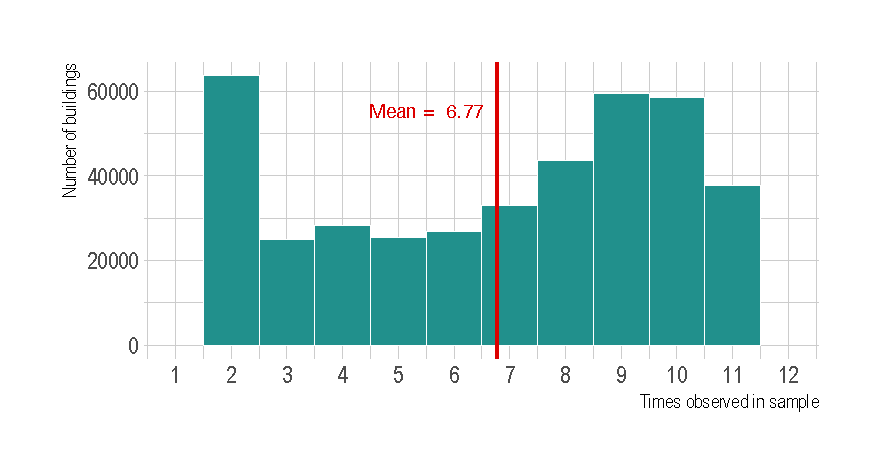
\includegraphics[width=0.75\linewidth]{figure/occurance_buildings} 

}

\caption{Number of occurrences of buildings in the full sample}\label{fig:occurrence-buildings}
\end{figure}
\textbf{Spatial and temporal coverage of sample}

In addition to how often an individual building is observed in the sample, also the spatial and temporal distribution of observations is of relevance. Figure \ref{fig:buildings-distribution} graphically depicts the spatial and temporal coverage of the full sample on the district-level.\footnote{Please note the use of the logarithmic scale in Figure \ref{fig:buildings-distribution}.} On the spatial dimension, the maps show that the coverage is good. There are very few districts without any building observed (transparent) and only a few districts with less than 10 buildings observed per year (dark blue). For most district-year combinations, more than 100 buildings are observed. In some large cities and metropolitan areas, numbers of more than 10,000 buildings annually are reached. The good spatial coverage of the data implies that results drawn from the sample have validity for Germany as a whole and are in their explanatory power not limited to certain regions or clusters.

On the temporal dimension, fewer observations are available in 2007 (43,696 observations) and 2008 (43,536 observations), as the energy price data was first included in these years. For the years between 2009 and 2019, an annual minimum of 201,856 and an average of 239,183 buildings are observed. Which means that the explanatory power of the results applies in particular to the period between 2009 and 2019. At the same time, exploratory testing of the data with and without consideration of the years 2007 and 2008 did not lead to a relevant change in the results meaning that the results are applicable to the whole time period under investigation.
\begin{figure}

{\centering 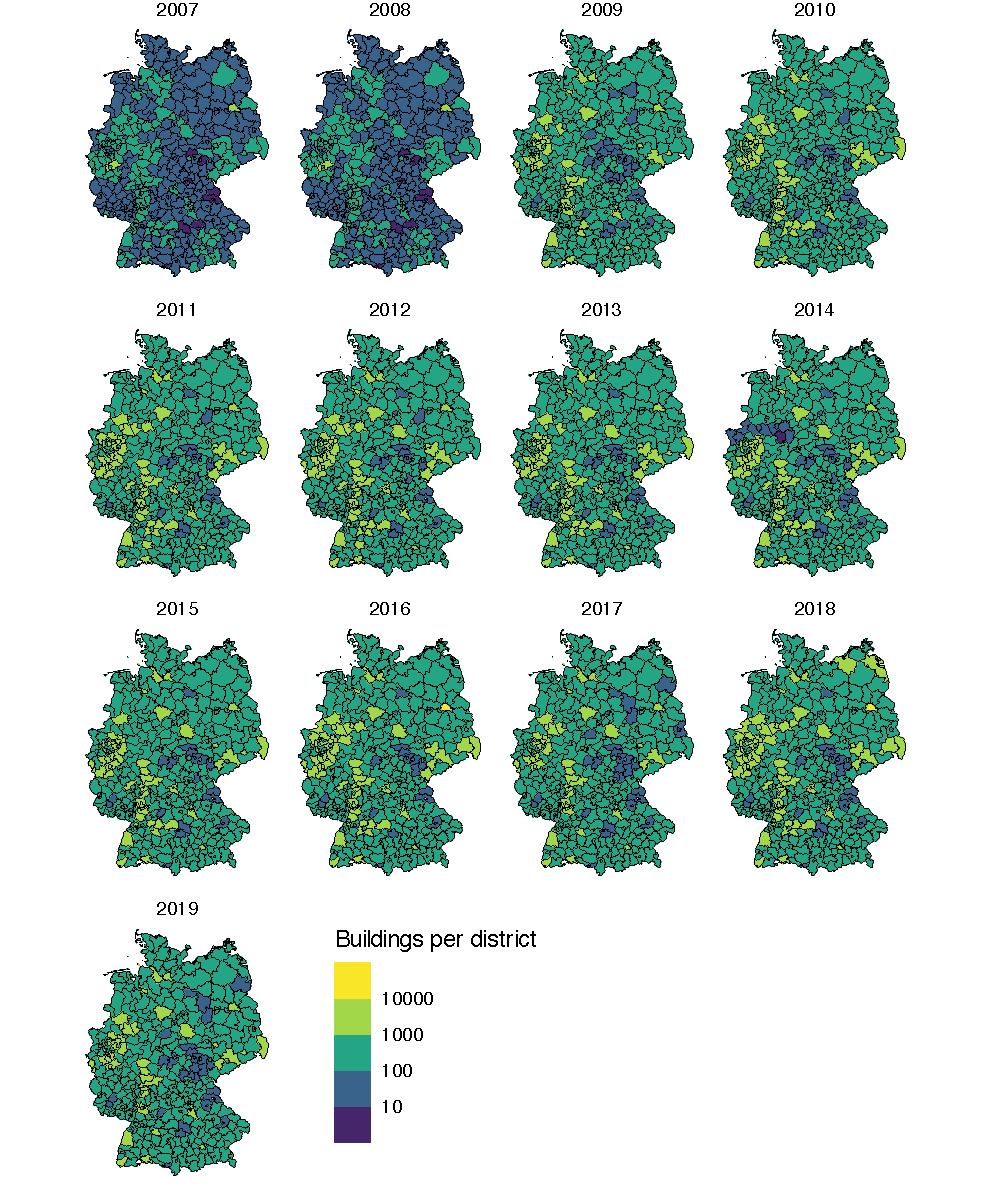
\includegraphics[width=0.77\linewidth]{figure/buildings_distribution} 

}

\caption{Spatial and temporal coverage by the buildings observed}\label{fig:buildings-distribution}
\end{figure}
\textbf{Summary statistics}

Table \ref{tab:summary-statistics} provides summary statistics for the full sample reporting the median values and the interquartile range (IQR). Besides the overall sample, also separate statistics for the three carrier types gas, oil, and district heating are included. About 60.6\% of the observations in the sample are associated with gas as the energy carrier. A further 29.5\% with oil and 9.9\% with district heating. For space heat demand, as the response variable, the median value (IQR) for the sample overall is 113 (86, 145) kWh/sqm/a and for energy price as the main explanatory variable the median (IQR) of the sample is 6.49 (5.77, 7.69) Cents/kWh.
\begin{table}[]
\centering
\caption{Summary statistics}
\label{tab:summary-statistics}
\resizebox{\textwidth}{!}{%
\begin{tabular}{@{}llllll@{}}
\toprule
Variable {[}Median (IQR){]} &
  Unit &
  \begin{tabular}[c]{@{}l@{}}Overall\\ N = 2,718,246\end{tabular} &
  \begin{tabular}[c]{@{}l@{}}Gas\\ N = 1,647,563 (60.6\%)\end{tabular} &
  \begin{tabular}[c]{@{}l@{}}Oil\\ N = 802,451 (29.5\%)\end{tabular} &
  \begin{tabular}[c]{@{}l@{}}District heating\\ N = 268,232 (9.9\%)\end{tabular} \\ \midrule
                                         &                 &                      &                      &                      &                      \\
Space heat demand, eff.                  & {[}kWh/sqm{]}   & 113 (86, 145)        & 116 (89, 149)        & 117 (91, 148)        & 83 (63, 109)         \\
Energy price, real                       & {[}Cents/kWh{]} & 6.49 (5.77, 7.69)    & 6.18 (5.56, 6.79)    & 7.06 (6.08, 8.25)    & 10.12 (8.71, 11.84)  \\
                                         &                 &                      &                      &                      &                      \\
Degree days                              &                 & 3,446 (3,214, 3,733) & 3,418 (3,192, 3,697) & 3,536 (3,273, 3,826) & 3,397 (3,191, 3,642) \\
Heating surface                          & {[}sqm{]}       & 404 (260, 707)       & 424 (271, 701)       & 305 (226, 466)       & 1,118 (556, 2,118)   \\
Housing units                            &                 & 6 (3, 10)            & 6 (3, 10)            & 4 (3, 6)             & 16 (8, 32)           \\
                                         &                 &                      &                      &                      &                      \\
\begin{tabular}[c]{@{}l@{}}District household income,\\ per capita\end{tabular} &
  {[}€/a{]} &
  20,695 (18,786, 22,568) &
  20,658 (18,731, 22,563) &
  21,098 (19,388, 22,861) &
  19,217 (17,667, 21,327) \\
District retirement share                & {[}\%{]}        & 0.207 (0.193, 0.220) & 0.209 (0.194, 0.222) & 0.205 (0.193, 0.216) & 0.210 (0.192, 0.230) \\
Postal code population density &
  \begin{tabular}[c]{@{}l@{}}{[}inhabitants/\\ sq. km{]}\end{tabular} &
  572 (217, 1,960) &
  662 (255, 2,121) &
  320 (149, 839) &
  2,053 (505, 4,821) \\ \midrule
\textit{Note: Median (IQR), No missings} &                 &                      &                      &                      &                      \\ \bottomrule
\end{tabular}%
}
\end{table}
In terms of energy demand and price, there are pronounced and relevant differences between the three types of energy carrier groups. The demand for gas and oil as energy carriers is higher than for district heating. The prices for gas are the lowest with relatively small fluctuations. Prices for oil are slightly higher, but show greater variation. Prices for district heating are by far the highest and also show the greatest variations. Additionally, buildings with a district heating system installed are three to four times the size of buildings with gas or oil heating installed (cf.~heating surface and housing units in Table \ref{tab:summary-statistics}). To check for potential multicollinearity issues between the variables Appendix \ref{fig:correlation-plot} shows a matrix of Pearson's correlation coefficients. None of the correlations observed between the variables exceed moderate values, which rules out any multicollinearity issues. Furthermore, the correlation matrix reveals that energy price is negatively correlated with energy demand, indicating that the expected negative relationship is reflected in the data.

\textbf{Focus on energy demand and prices}

Figure \ref{fig:demand-descriptive-graph} provides a more detailed visual summary of the demand variable. The aggregated demand distribution of the three carrier types and years tapers off towards the upper end. The lowest annual demands are around 25 kWh/sqm/a. The distribution peaks at just over 100 kWh/sqm/a and then tapers off to very high demand values of up to 350 kWh/sqm/a (Panel A). With a differentiated display by energy carrier (Panel B), the graph confirms the findings from Table \ref{tab:summary-statistics}. While the demands for gas and oil are on an almost similar higher level, demand in buildings with district heating is considerably lower. The major share of this difference in demand is most likely attributable to the difference in building size. Because buildings heated with district heating are on average three to four times larger than buildings with oil or gas heating, they have a better ratio of heating area to building exterior area, resulting in lower heat losses per square meter heated. Given the significance of the difference in demand, it was further scrutinized if the age of the building and the age of the heating system may deviate between gas and oil buildings on the one side and buildings with district heating on the other side. Newer buildings and newer heating systems would be expected to go along with lower energy demand. Appendix \ref{tab:age-building-heating-system} provides this comparison, which finds no differences between energy carriers of a magnitude that would suggest a strong impact on demand.
\begin{figure}

{\centering 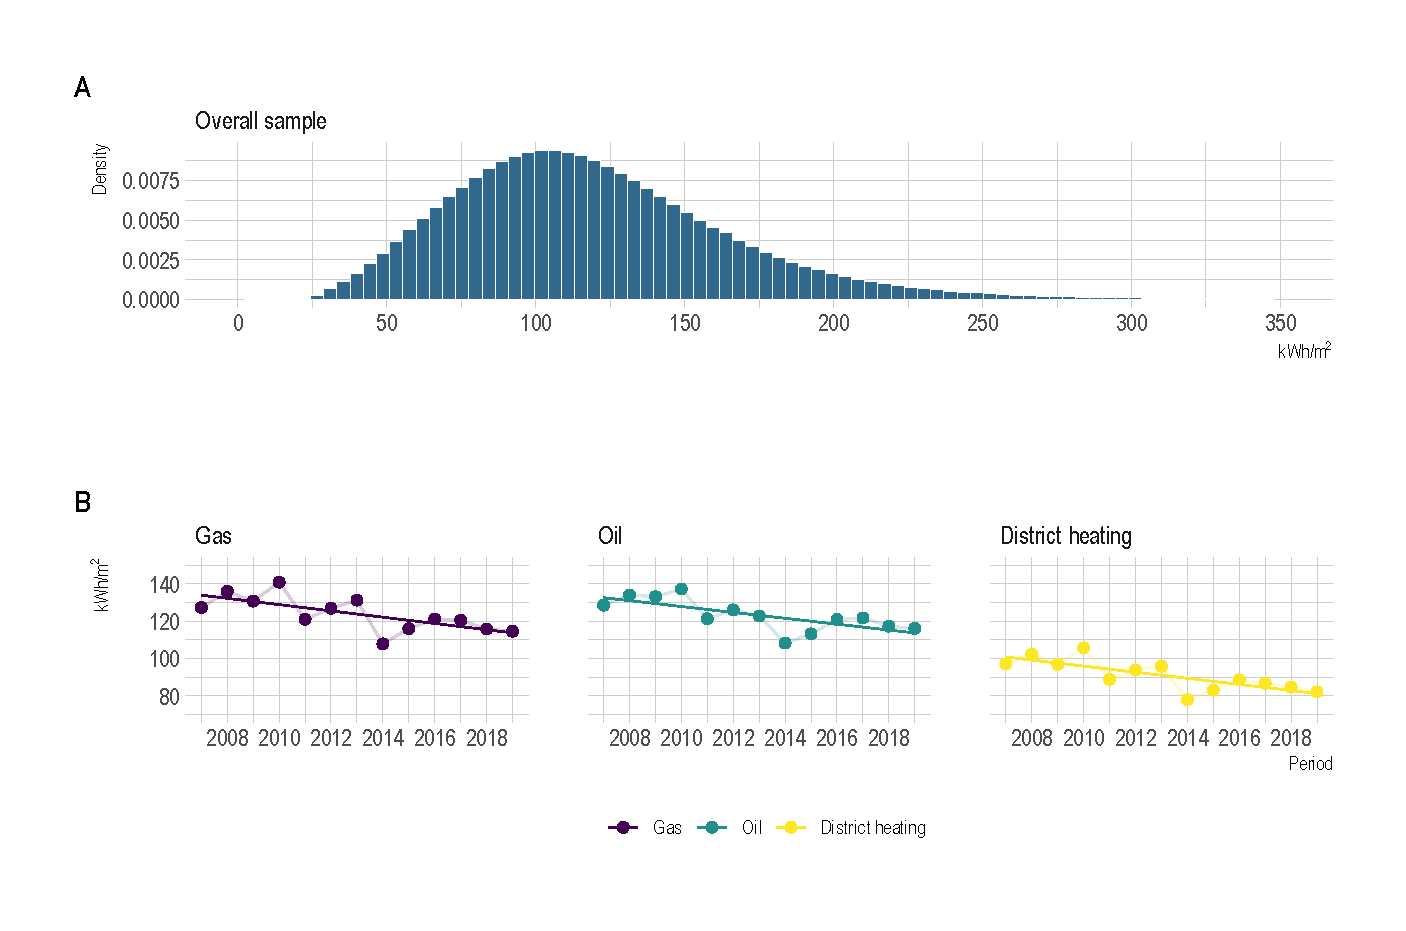
\includegraphics[width=1\linewidth]{figure/demand_descriptive} 

}

\caption{Distribution of energy demand}\label{fig:demand-descriptive-graph}
\end{figure}
In addition, Panel B of Figure \ref{fig:demand-descriptive-graph} provides two additional relevant pieces of information regarding the energy demand variable. First, for all three carrier types the effective demand decreases over time. This is most likely due to multiple factors one of which would be the demand response investigated in this thesis. Additionally, over time, newer more energy efficient buildings are added to the sample, while old and more inefficient building stock likely drops from the sample. Furthermore, the building stock remaining in the sample may undergo renovation measures leading to lower energy demand. Lastly, increasing outside temperatures due to climate change may also lead to the decline in effective demand observed. Linked to the role of climatic conditions is also a second aspect which can also be derived from the graph: Effective demand follows a similar pattern for all carriers, which can, however, also turn out to be higher or lower from year to year and only declines in the overall trend. Fluctuations in effective energy demand are linked to the variations in climatic conditions. In Appendix \ref{fig:degree-days-distribution} the distribution of degree days is depicted on a spatial and temporal scale. There is a consistent trend between degree days and energy demand that corroborates the intuition that higher degree days (lower outside temperatures) leads to higher energy demand. This illustrates the relevance of considering climatic conditions as an additional determinant of space heating demand.

Figure \ref{fig:price-descriptive-graph} depicts the distribution of nominal (Panel A) and real (Panel B) energy prices also by energy carrier. The points represent the average price in one year. The vertical bars represent the standard deviation. While the energy prices for gas are relatively stable over the period under observation, prices for oil show stronger volatility. As already established previously, prices for district heating are higher than those for gas and oil (cf.~Table \ref{tab:summary-statistics}). Furthermore, the prices for district heating are not as volatile, but show a huge range of variation, which is reflected in the much larger standard deviations.
\begin{figure}

{\centering 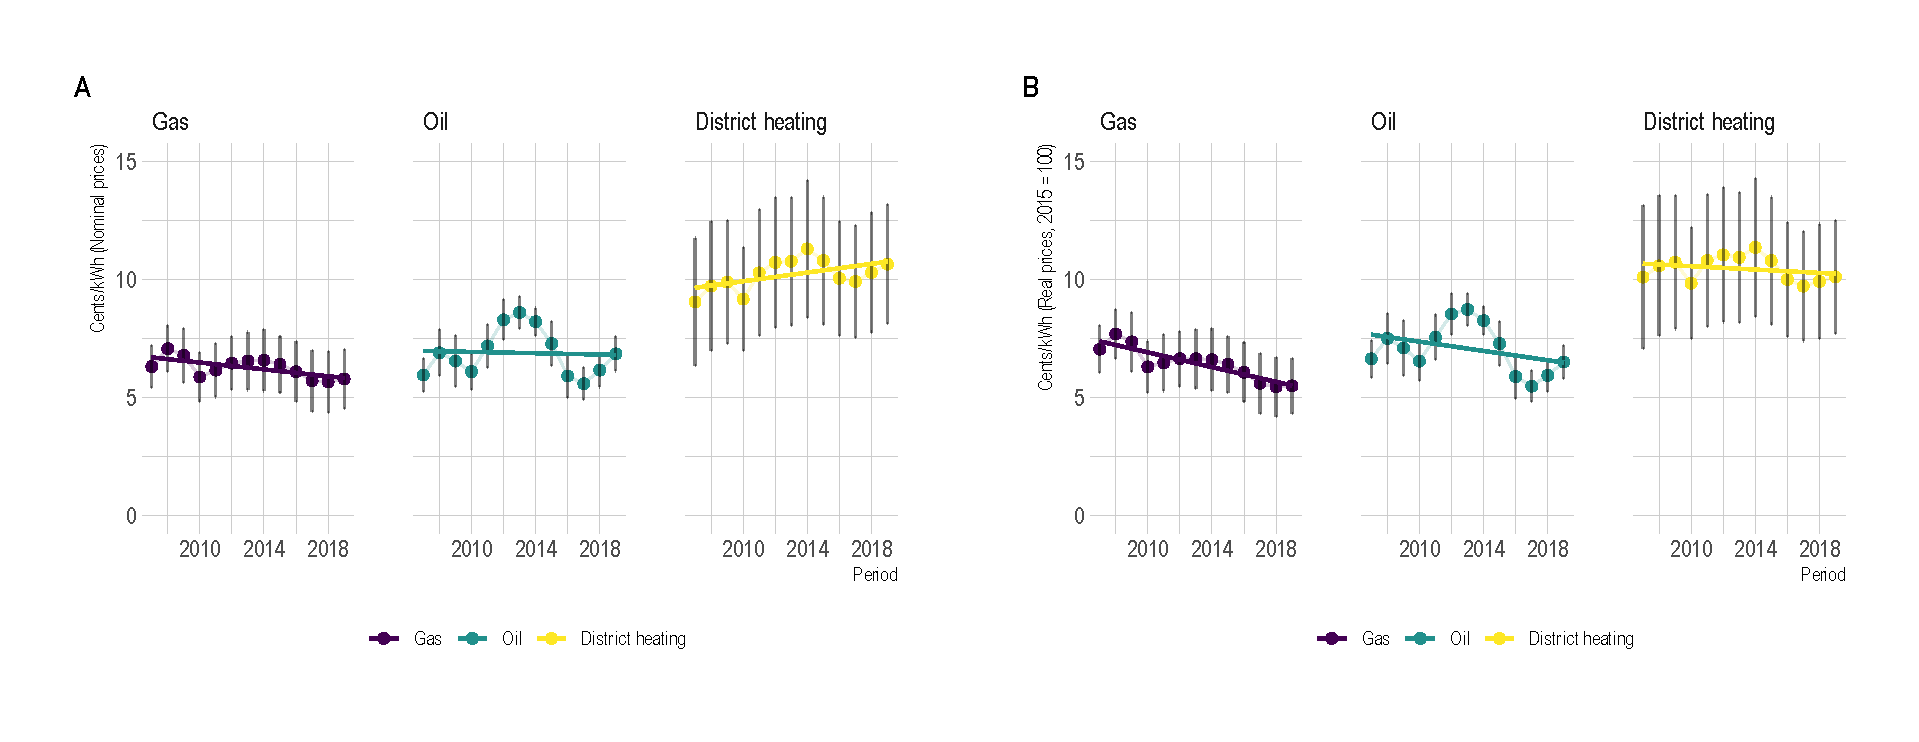
\includegraphics[width=1\linewidth]{figure/prices_descriptive} 

}

\caption{Distribution of nominal and real energy prices}\label{fig:price-descriptive-graph}
\end{figure}
While nominal prices are relatively stable in the overall trend for all three energy carrier groups, the trend changes after adjusting for inflation. The deflated real prices show an overall declining trend, with the trend being more pronounced for gas and oil. For the intuition about the price elasticity of space heating demand, this means that one would expect an overall increase in demand from the price effect alone. However, the graph also shows that effects into both directions can be observed when looking not at the overall trend but at year-to-year movements.

After having described the data and energy demand and energy prices as the two main variables in detail, the following Chapter will present the results of the regression analysis.

\hypertarget{results}{%
\chapter{Results}\label{results}}

The results Chapter is structured in two subsections. First, the results from the analysis of the full sample are presented (reflects first part of workflow, see Figure \ref{fig:workflow1}). And subsequently the results of the deepened analysis based on the stratified subsample are reported (reflects the second part of the workflow, see Figure \ref{fig:workflow2}).

\hypertarget{full_sample_results}{%
\section{Full sample results}\label{full_sample_results}}

\textbf{Price elasticity estimates}

The results of the full sample analysis are shown in Table \ref{tab:reg-table}. The overarching finding regarding the price elasticity of space heating demand is that the elasticities in all model specifications are \emph{negative} and \emph{relatively inelastic}. On the one hand, the price elasticities being negative confirms that the basic intuition of falling demand with rising prices is reflected in the data. The relative inelastic magnitude of the demand response, on the other hand, validates the assumption derived from the literature that space heating in private households -- especially in the short-term -- is an inelastic good.

Specifications (m1.ols) and (m2.ols) are the cross-sectional models based on the OLS estimator. Interestingly, the energy price coefficient remains stable when moving from Specification (m1.ols) with price as the only predictor of space heating demand to Specification (m2.ols) where the set of additional control variables is added to the model. The price elasticity coefficient in Specification (m2.ols) is to be interpreted that a 1\% increase in energy price leads to a -0.365\% reduction in space heating demand.
\begin{table}[]
\centering
\caption{Regression table for full sample analysis}
\label{tab:reg-table}
\resizebox{\textwidth}{!}{%
\begin{tabular}{llrrrrrrr}
\cline{3-9}
 &  & \multicolumn{7}{c}{\begin{tabular}[c]{@{}c@{}}Response variable in all model specifications:\\ Ln of space heat demand\end{tabular}} \\
 &  & \multicolumn{2}{c}{OLS} & \multicolumn{1}{c}{} & \multicolumn{4}{c}{Fixed Effects (FE)} \\
 &  & \multicolumn{1}{c}{(m1.ols)} & \multicolumn{1}{c}{(m2.ols)} & \multicolumn{1}{c}{} & \multicolumn{1}{c}{(m1.fe)} & \multicolumn{1}{c}{(m2.fe)} & \multicolumn{1}{c}{(m3.fe)} & \multicolumn{1}{c}{(m3.fe, lagged)} \\ \cline{1-1} \cline{3-4} \cline{6-9} 
(Intercept) &  & 5.399 *** & 3.593 *** &  &  &  &  &  \\
 &  & (0.002) & (0.028) &  &  &  &  &  \\
\begin{tabular}[c]{@{}l@{}}Ln of\\ energy price\end{tabular} &  & -0.365 *** & -0.365 *** &  & -0.251 *** & -0.243 *** & -0.243 *** &  \\
 &  & (0.001) & (0.001) &  & (0.001) & (0.001) & (0.001) &  \\
\begin{tabular}[c]{@{}l@{}}Ln of lagged\\ energy price (t-1)\end{tabular} &  &  &  &  &  &  &  & -0.071 *** \\
 &  &  &  &  &  &  &  & (0.001) \\
\begin{tabular}[c]{@{}l@{}}Ln of\\ degree days\end{tabular} &  &  & 0.626 *** &  &  & 0.779 *** & 0.779 *** & 0.850 *** \\
 &  &  & (0.002) &  &  & (0.003) & (0.003) & (0.004) \\
\begin{tabular}[c]{@{}l@{}}Ln of \\ heating surface\end{tabular} &  &  & -0.133 *** &  &  & -0.405 *** & -0.405 *** & -0.408 *** \\
 &  &  & (0.000) &  &  & (0.003) & (0.003) & (0.004) \\
\begin{tabular}[c]{@{}l@{}}Energy carrier:\\ Oil\end{tabular} &  &  & 0.031 *** &  &  & 0.097 *** & 0.097 *** & 0.074 *** \\
 &  &  & (0.001) &  &  & (0.002) & (0.002) & (0.002) \\
\begin{tabular}[c]{@{}l@{}}Energy carrier:\\ District heating\end{tabular} &  &  & -0.061 *** &  &  & -0.020 *** & -0.020 *** & -0.067 *** \\
 &  &  & (0.001) &  &  & (0.002) & (0.002) & (0.003) \\
\begin{tabular}[c]{@{}l@{}}Ln of district\\ per capita household income\end{tabular} &  &  & -0.277 *** &  &  & 0.022 ** & 0.022 ** & 0,015 \\
 &  &  & (0.002) &  &  & (0.008) & (0.008) & (0.010) \\
District retirement share &  &  & -0.084 *** &  &  & 0.435 *** & 0.435 *** & 0.418 *** \\
 &  &  & (0.010) &  &  & (0.030) & (0.030) & (0.037) \\
\begin{tabular}[c]{@{}l@{}}Postal code\\ population density\end{tabular} &  &  & 0.043 *** &  &  & 0,000 &  &  \\
 &  &  & (0.000) &  &  & (0.005) &  &  \\ \cline{1-1} \cline{3-4} \cline{6-9} 
N &  & 2718246 & 2718246 &  & 2718246 & 2718246 & 2718246 & 2020628 \\
R2 &  & 0,049 & 0,156 &  & 0,822 & 0,829 & 0,829 & 0,847 \\
logLik &  & -1322263,852 & -1159565,133 &  &  &  &  &  \\
AIC &  & 2644533,703 & 2319150,267 & \multicolumn{1}{l}{} & \multicolumn{1}{l}{} & \multicolumn{1}{l}{} & \multicolumn{1}{l}{} & \multicolumn{1}{l}{} \\ \cline{1-1} \cline{3-4} \cline{6-9} 
*** p \textless 0.001;  ** p \textless 0.01;  * p \textless 0.05. &  & \multicolumn{1}{l}{} & \multicolumn{1}{l}{} & \multicolumn{1}{l}{} & \multicolumn{1}{l}{} & \multicolumn{1}{l}{} & \multicolumn{1}{l}{} & \multicolumn{1}{l}{}
\end{tabular}%
}
\end{table}
When moving from the OLS estimator to the fixed-effects (FE) estimator in Specifications (m1.fe) - (m3.fe), the estimated price elasticities of demand become more inelastic. This effect is in line with what, for example, also \protect\hyperlink{ref-miller_alberini16}{Miller \& Alberini} (\protect\hyperlink{ref-miller_alberini16}{2016}) find when moving from a cross-sectional model to the use of unit-level fixed effects. The reason for this is probably unobserved factors at the building level that are not fully reflected in the building characteristics controlled for, as well as temporal effects. This time, moving from Specification (m1.fe) with price as the sole predictor of space heating demand to Specification (m2.fe) which also includes the other predictor variables, the coefficient of energy price becomes slightly more inelastic but the effect in magnitude remains minor. Specification (m3.fe) drops the population density from the equation since it is found to have no effect in Specification (m2.fe). Thus, Specification (m3.fe) reflects the final model for the full sample analysis. The price elasticity coefficient in Specification (m3.fe) is to be interpreted that a 1\% increase in energy price leads to a -0.243\% reduction in space heating demand. The results for the price elasticity of demand are of a comparable magnitude to previous evidence in the literature (see Figure \ref{fig:literature-estimates-plot}).

Specification (m3.fe, lagged), also shown in the table, shows the results for the case that not the energy price in the same period, but the price in the previous period (communicated through the energy bill of the previous year) influences the demand decision of households. When the lagged energy price is used as a predictor, the magnitude of the demand response is reduced to one third of the effect size: from -0.243\% when using the price in \(t\) to -0.071\% for the price in \(t-1\) (contingent on a 1\% increase in energy prices). While the demand response is still negative, this represents a major reduction in magnitude of the effect. In the literature, there are varying rationales on whether the price in the same or in previous periods informs demand decisions for space heat. In this study I follow the approach of \protect\hyperlink{ref-schmitz_madlener20}{Schmitz \& Madlener} (\protect\hyperlink{ref-schmitz_madlener20}{2020}) and assume that prices in the same period drive demand levels. However, the results for when using the price in previous billing period are reported to obtain a more comprehensive picture on the price elasticity estimates. Importantly, it should be noted that part of the difference between the estimates may also be due to the fact that in Specification (m3.fe, lagged) about 0.7 million fewer observations are included in the estimation, since a building must occur in the sample in two consecutive periods (energy price in \(t-1\) and energy demand in \(t\)) for an observation to be included. This exclusion criterion may lead to some type of selection bias, where buildings with certain characteristics that continuously appear in the sample are more heavily represented.

\textbf{Other estimates and effects}

In general, almost all model predictors are found to be statistically significant with a p-value \textless{} 0.1\%. However, this is not surprising given the very large number of more than 2.7 million observations (\protect\hyperlink{ref-gelman_stern06}{Gelman \& Stern, 2006}; \protect\hyperlink{ref-johnson99}{Johnson, 1999}). Besides the interpretation of the price elasticities, the signs of the other relevant model predictors also point in the expected direction (see rationales established in Chapter \ref{conceptual-model}). As most of the predictors are also included in the model in the ln-form, they can as well be interpreted in terms of percentage point change.

Referring again to the main model Specification (m3.fe), this means that, for example, a rise in degree days (lower outside temperatures) of 1\% would be associated with to a higher energy demand of 0.779\% and a larger building heating surface of 1\% would be associated with a lower energy demand of -0.405\%. Furthermore, the results indicate that an oil heating system is associated with a higher heating energy demand than gas as the reference category and a district heating system with a lower demand. While the results in the cross-sectional OLS model indicate that an increasing district per capita household income would be associated with a decreasing energy demand, this effect disappears in the FE model and is even reversed. At the same time, the magnitude of the district per capita household income effect in Specification (m3.fe) is so small that one must assume that it does not have a strong influence in explaining the variance in energy demand at all. For district retirement share the sign of the coefficient as well switches when moving from the OLS to the FE model. The results in Specification (m3.fe) indicate that a higher district level retirement share is associated with higher energy demand.

\hypertarget{subsample_results}{%
\section{Subsample results}\label{subsample_results}}

\textbf{Price elasticity estimates}

Figure \ref{fig:posterior-distributions} summarizes the posterior distributions for the price elasticities of space heating demand in the Bayesian models (see Figure \ref{fig:workflow2} to compare which model structure and predictor is used in the respective Specification). The complete model summaries -- going beyond the price coefficients -- are reported in Appendix \ref{tab:brms-full-model-results}.

Also for the Bayesian models, the estimates for the price elasticity of space heating demand are in the negative and relatively inelastic range. In contrast to the results of the total sample, however, it is noticeable that the price elasticities found in the subsample are more elastic. This could be partly due to the alternative modelling approach. But probably it is mainly the different composition of the sample that causes the difference in the estimates. That the overall findings of the full and subsample analysis agree well is also evident from the fact that the trend towards lower estimates for the price elasticity is the same when additional predictors are included and when controlling for the group-level effects of buildings and time.

Specifications (b.1) and (b.2) represent the simpler model design without varying intercepts. In Specification (b.1), with energy price as the sole predictor of energy demand, the price elasticity is estimated to be -0.56 {[}-0.59; -0.53{]} (Mean estimate {[}95\% CI{]}). When moving to Specification (b.2) where the additional explanatory variables are added, the estimate moves to -0.41 {[}-0.45; -0.38{]} and thus becomes wider and less price responsive (inelastic). Again, using the results from Specification (b.2) as an example, the price elasticity coefficients are o be interpreted that a 1\% increase in energy price leads to a -0.41\% {[}-0.45; -0.38{]} reduction in space heating demand.
\begin{figure}

{\centering 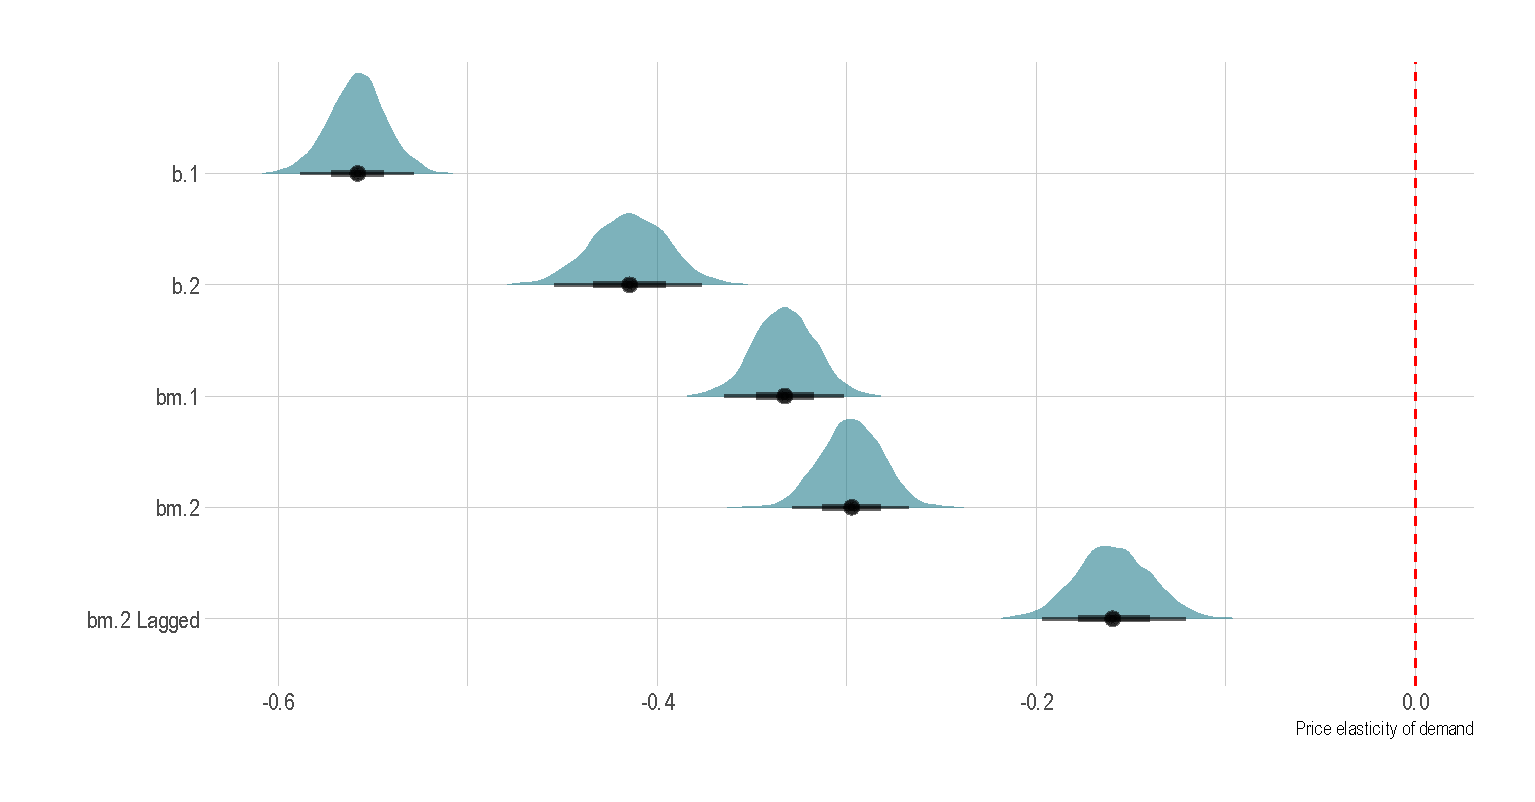
\includegraphics[width=1\linewidth]{figure/posterior-distributions} 

}

\caption{Posterior distributions for the price elasticities of space heating demand based on the subsample}\label{fig:posterior-distributions}
\end{figure}
In the more sophisticated specifications involving multilevel partial pooling for buildings and years (bm.x models), the price elasticities become lower, similar to the FE models in the full sample analysis. In Specification (bm.1) energy price is used as a sole predictor and group-level terms are included. In Specification (bm.2) the additional explanatory variables are included. The inclusion of the additional variables resulted in divergent transitions caused by the heating area and population density variables. Therefore, the two were excluded from the model to ensure convergence and reliability of results. In Specification (bm.2) the estimate for the price elasticity of space heating demand is -0.30 {[}-0.33; -0.27{]}, meaning that a 1\% increase in energy price would lead to a -0.30\% {[}-0.33; -0.27{]} reduction in space heating demand. Also similarly to the full sample analysis, the by far lowest estimate is found when using the lagged energy price variable (\(t-1\)) instead of the energy price in the same period (\(t\)) to explain the variance in space heat demand. For Specification (bm.2 Lagged) the estimate is -0.16 {[}-0.20; -0.12{]}.

Generally, it should be noted that due to the varying representation of energy carriers between the full- and the subsample, a direct comparison of the resulting estimates is not sensible. In the full sample there is a larger representation of observations relying on a gas heating system and fewer observations with a district heating system. These differences are removed by the stratified sampling approach.

\textbf{Re-scaling elasticity results to the demand scale and integrating prediction intervals to convey uncertainty}

Figures \ref{fig:elasticity-predictions-b1} and \ref{fig:elasticity-predictions-bm2} illustrate what the differences found in the price elasticity estimates imply when being converted back to the actual scale of demand. Figure \ref{fig:elasticity-predictions-b1} shows predictions for the basic Specification (b.1) where energy price acts as the sole predictor of space heating demand and group-level differences between buildings and years are not yet considered. Panel A on the left shows the observations in the subsample with model predictions on the ln-scale. Panel B on the right shows the re-scaled values on the scale of actual demand.\footnote{Values are re-scaled using \(exp()\).}
\begin{figure}

{\centering 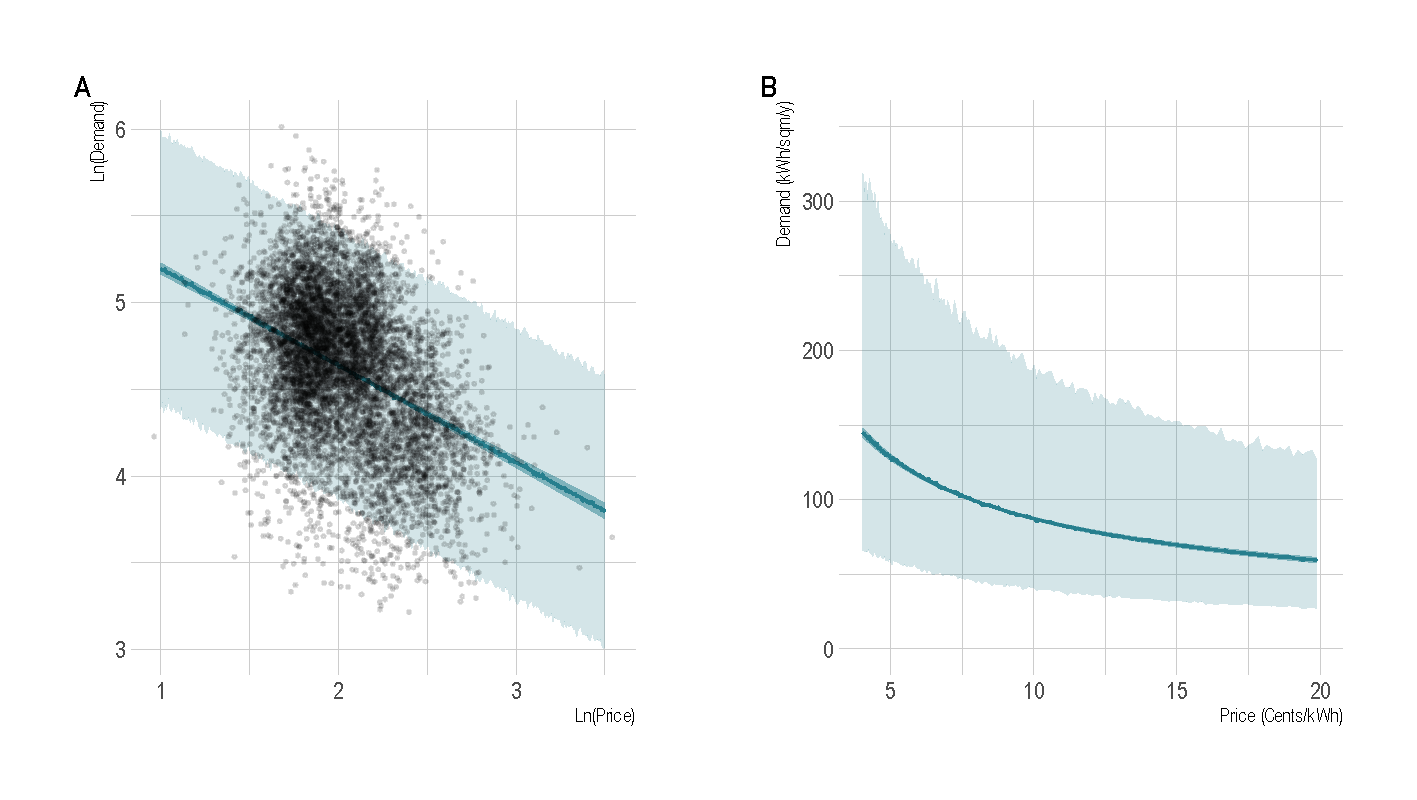
\includegraphics[width=1\linewidth]{figure/b1_prediction} 

}

\caption{Predicted price elasticities of space heating demand based on simple model (b.1)}\label{fig:elasticity-predictions-b1}
\end{figure}
Methodologically, the line in the center represents the average energy demand at a respective price. The narrower, darker shaded interval around the mean represents the 95\% intervals for the posterior distribution of the expected value of the demand parameter \(\mu\) (see Chapter \ref{empirical-model}). These posterior predictive distributions have a lower variance because only the uncertainty of the mean is included in the draws, but the residual error is ignored. The wider, lighter shaded interval, on the other hand, represents the posterior predictive distributions including the residual error. It is thus to be interpreted as the interval in which the model expects to find 95\% of the actual energy demands in the population at each price.\footnote{Cf. \protect\hyperlink{ref-mcelreath20}{McElreath} (\protect\hyperlink{ref-mcelreath20}{2020}), Chapter 4 and the brms documentation on the \(posterior.epred\) and \(posterior_predict\) functions in R for the interpretation of the posterior predictive intervals shown in the graph.}

The two types of prediction intervals convey two types of uncertainty: uncertainty in the parameter value (darker shaded interval) and uncertainty in the sampling process (lighter shaded interval). The distribution of simulated outcomes (lighter shaded interval) includes sampling variation and therefore indicates what the future data would look like (\protect\hyperlink{ref-mcelreath20}{McElreath, 2020}). In other words, it tells us what demand levels can be expected at different prices in a population of German multi-apartment buildings with equal shares of the three energy carriers gas, oil and district heating. The lighter shaded intervals are therefore the most important intervals for interpretation. It should be noted, however, that due to the stratified sampling procedure used to create the subsample, the interpretations are only generalisable to a limited extent, as the relative shares of the energy carriers do not reflect the shares in the actual building stock.

For the simple Specification (b.1) in Figure \ref{fig:elasticity-predictions-b1}, the mean space heating demand expected by the model drops from about 150 kWh/sqm/year at a price of 4 cents/kWh to about 60 kWh/sqm/year at a price of 20 cents/kWh.\footnote{Note that the price range shown in the graph were chosen arbitrarily to some extent. They were chosen to represent the lowest reasonable price at the low end and to reflect about 2-3 times the historical prices observed in the sample at the high end.} In addition to the mean, the intervals show well the uncertainty associated with the model predictions. For the low end of the chosen price range at 4 cents/kWh, the model expects 95\% of the actual energy demand of the population to be between 70 and 315 kWh/sqm/year, which is obviously a very wide range. At the upper end of the price range, the predicted interval narrows. At 20 cents/kWh, the model expects 95\% of the actual energy demand to be in the range between 35 and 130 kWh/sqm/year. Overall, the predictions of the simple model thus show the negative relationship between price and demand, but are still subject to large uncertainty due to the residual error of the model.
\begin{figure}

{\centering 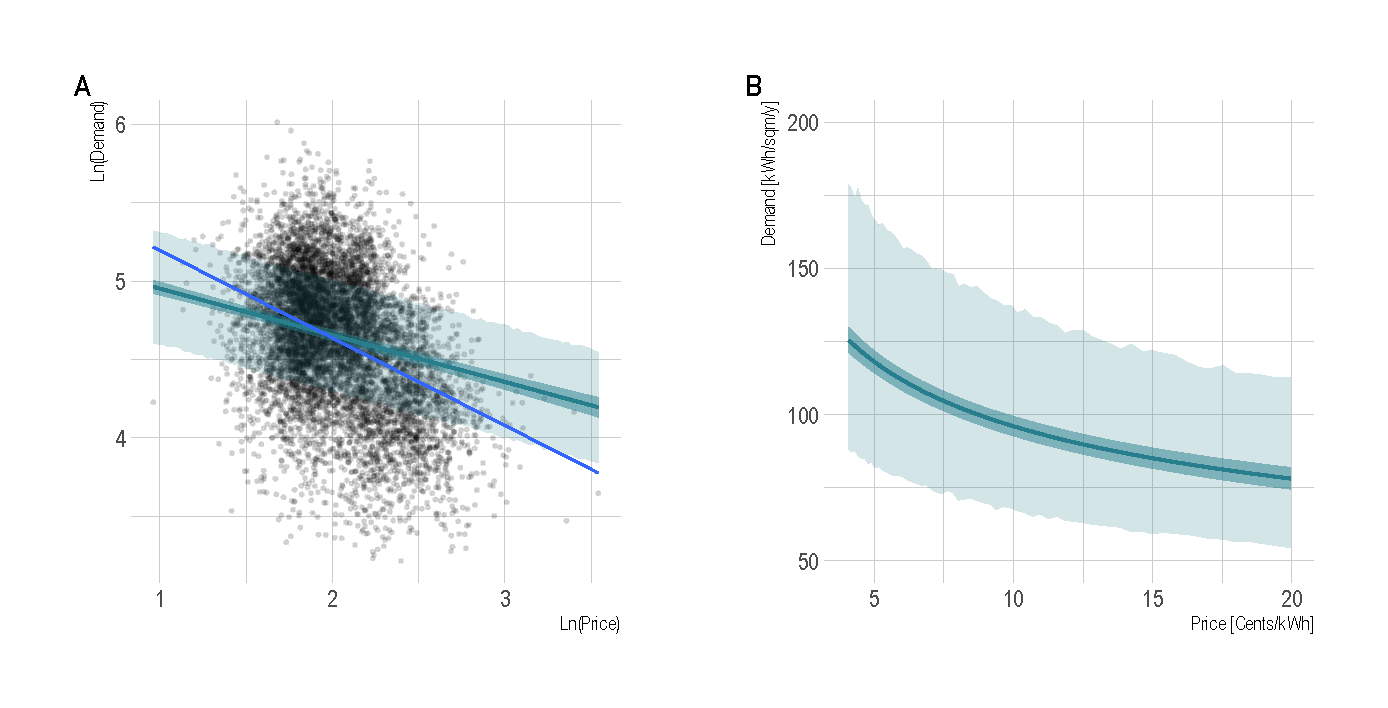
\includegraphics[width=1.04\linewidth]{figure/bm2_prediction} 

}

\caption{Predicted price elasticities of space heating demand based on multilevel partial pooling model (bm.2)}\label{fig:elasticity-predictions-bm2}
\end{figure}
Figure \ref{fig:elasticity-predictions-bm2} presents the same type of figure, but relies on the multilevel partial pooling model from Specification (bm.2). The additional blue line in Panel A represents the simple linear model between price and demand. The different trajectory between the simple linear model (blue line) and the prediction for the model Specification (bm.2) (green line) shows that the inclusion of the additional explanatory variables and the group-level pooling for buildings and years has a strong impact on the prediction. The predicted elasticity is less elastic and the intervals are much narrower. On the demand scale, again shown in Panel B, the average energy demand predicted by the model drops from about 125 kWh/sqm/year at a price of 4 cents/kWh to about 80 kWh/sqm/year at a price of 20 cents/kWh. Moving to the simulated results (lighter shaded intervals), the model expects 95\% of the actual energy demand in the population to be between 85 and 175 kWh/sqm/year for the lower end of the price range shown at 4 cents/kWh. At the higher end, at a price of 20 cents/kWh, the interval narrows again to 55 to 110 kWh/sqm/year. Thus, the intervals have become much narrower, indicating that the prediction of Specification (bm.2) provides a more realistic picture on the interplay between energy price and demand as compared to the prediction from the simple model in Specification (b.1).

Overall, the figures provide a good indication of what the reported price elasticities of space heating demand would mean in practice, given a range of realistic price levels.

\textbf{Investigation of potential heterogeneity in price responsiveness}

While the results presented thus far for the subsample largely mirror the procedure used for the full sample analysis, but based on Bayesian inference and using a different sample composition, the final part of the subsample analysis aims to go further by examining potential sources of heterogeneity in the price responsiveness. This is done in two steps. First, the variables used in the analysis are examined for potential heterogeneity relying on graphical representations. Second, the heterogeneity found visually for the different energy carrier groups is then being formalized in a regression analysis by means of extending Specification (bm.2) by a interaction term between energy price and energy carrier groups.

For the first part, the visual examination of potential heterogeneity in price responsiveness, the following variables are considered: year, federal state, energy carrier group, degree days, heating surface, district per capita household income, and district retirement share.\footnote{Note that postal code population density was not considered because it was neither included in the final model for the analysis of the full sample (Specifications (m2.fe)) nor in the final model for the analysis of the subsample (Specifications (bm.2)).} For the categorical variables years and federal states the graphs are shown in Appendix \ref{fig:heterogeneity-year-state-plot}. The observations in the subsample are grouped by year or federal state and presented in a scatter plot between energy price and demand. The lines represent simple linear models for each grouped category of year or federal state. For the years variable, the graph well indicates that the energy demand in the sample is lower overall in the later periods. With regard to potential heterogeneity in price elasticity between the years, however, no significant differences can be identified. The lines for all years follow more or less the same slope. The same is true for the federal state variable. While there are some differences between the individual states, there is no pattern of strongly diverging price elasticities of space heating demand.

Similarly, Appendix \ref{fig:other-variables-heterogeneity-plot} presents the visual examinations for the variables degree days, heating surface, district per capita household income, and district retirement share. Since all four variables are continuous, they are each divided into three equally sized groups to be able to investigate possible heterogeneity in the price response visually (e.g., one third of observations with highest number of degree days, one third with medium number of degree days, one third of observations with lowest number of degree days). For the two variables degree days and district retirement share, the three grouped lines are almost completely parallel, suggesting that there are no differences in the price response between the groups. For district per capita household income minor differences can be observed. Districts with a lower per capita household income exhibit a more elastic demand response (steeper slope). For the building heating surface as well some differences can be found with larger buildings being associated with a more elastic demand response than smaller buildings.
\begin{figure}

{\centering 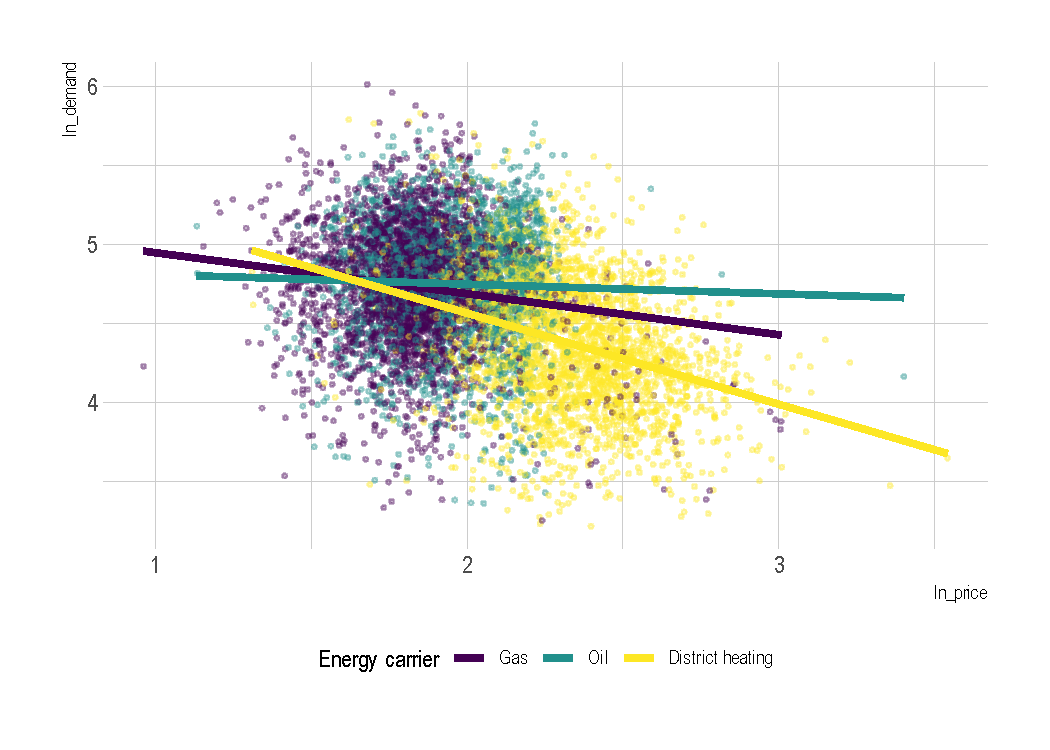
\includegraphics[width=0.8\linewidth]{figure/carrier_heterogeneity_plot} 

}

\caption{Investigation of heterogeneity between energy carrier groups}\label{fig:heterogeneity-energy-carrier-plot}
\end{figure}
In addition, the energy carrier group was investigated for potential differences between the three carrier types (oil, gas, district heating). The results are shown in Figure \ref{fig:heterogeneity-energy-carrier-plot}. The differences in the price responsiveness between the energy carrier groups are most pronounced. For buildings with oil heating, demand is almost constant, which indicates that they do not adjust their energy demand to a large extent to a change in the oil price. Buildings with gas heating show a moderate demand response to price changes. And buildings with district heating have by far the most elastic demand response when relying on the simple linear relationship shown in the graph.

Based on the visual examination of the variables, the findings were used to construct a better fitting model which integrates heterogeneity in price responsiveness by adding an interaction term. Since the visual analysis revealed that there were no heterogeneity detected between varying years, federal states, degree days and district retirement shares, these variables were not probed further. The heterogeneity found between the energy carrier groups but also among the district per capita household income and building heating surface variables were assessed further. Exploratory testing of models showed that interacting energy price with district per capita household income showed no relevant difference. Furthermore, interacting energy prices with building heating surface lead to non-convergence of model results and was therefore not further pursued. Interacting energy price with the energy carrier group, however, lead to relevant differences for the price elasticity pared with a converging model.

The posterior distributions for the price elasticities of space heating demand for the additional estimated interaction model Specification (bm.3) are shown in Figure \ref{fig:posterior-distribution-interaction}. The different posterior distributions reflect the results of the visual examination of the simple linear relationship. The most inelastic demand response is found for buildings with oil heating -0.16 {[}-0.23; -0.10{]} (Mean estimate {[}95\%CI{]}). For buildings with gas as the energy carrier type, the estimates are in a medium range of -0.35 {[}-0.40; -0.29{]}. For buildings with district heating, demand is most elastic with estimates of -0.53 {[}-0.60; -0.46{]}. Also the width of the distributions provides some insights. For gas and district heating as energy carriers the posterior distribution is wider than for oil. This is likely due to the observations for gas and district heating to be more widely spread (see also the previous Figure \ref{fig:heterogeneity-energy-carrier-plot}).
\begin{figure}

{\centering 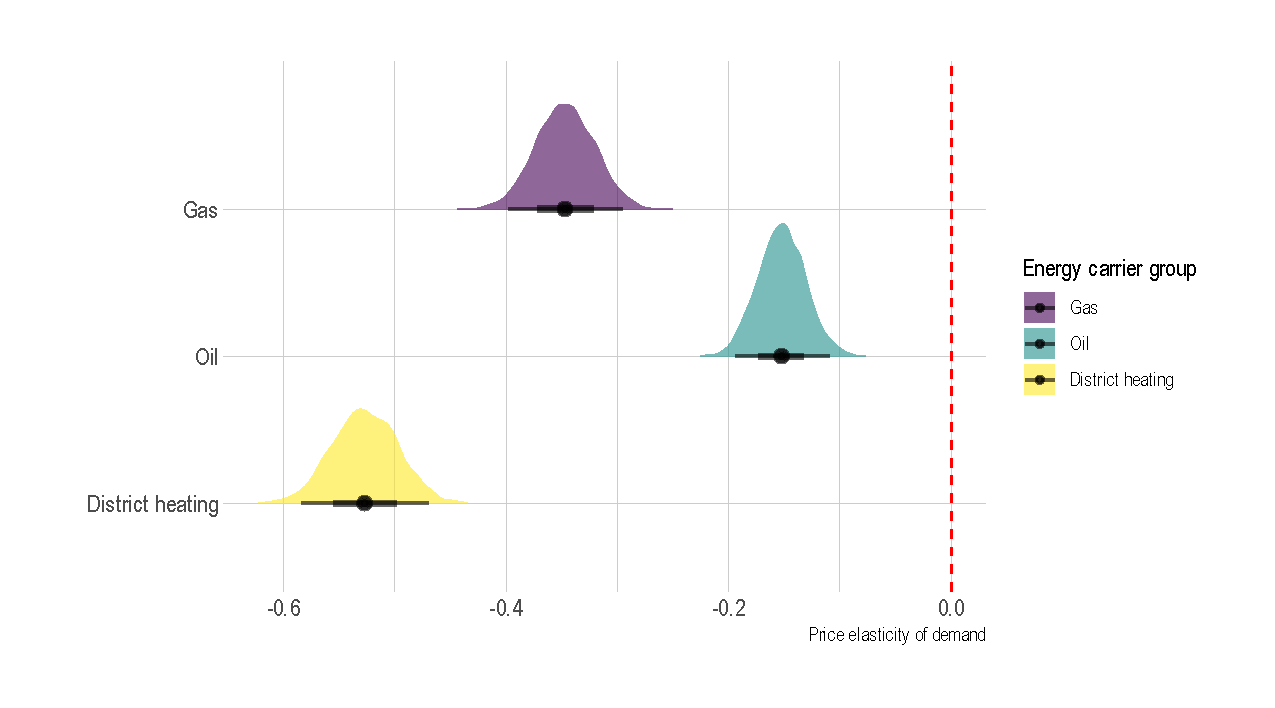
\includegraphics[width=1\linewidth]{figure/posterior-distribution-interaction} 

}

\caption{Posterior distributions for the price elasticities of space heating demand by energy carrier group based on the subsample}\label{fig:posterior-distribution-interaction}
\end{figure}
Mirroring the approach taken for the model not interacting energy price with energy carrier group, the results from model Specification (bm.3) are as well translated to Figure \ref{fig:elasticity-predictions-energy-carrier} involving prediction intervals. Also here the inner darker shaded intervals represent uncertainty in the parameter value and the lighter shaded intervals uncertainty in the sampling process and thus including the residual error of the model (\protect\hyperlink{ref-mcelreath20}{McElreath, 2020}).
\begin{figure}

{\centering 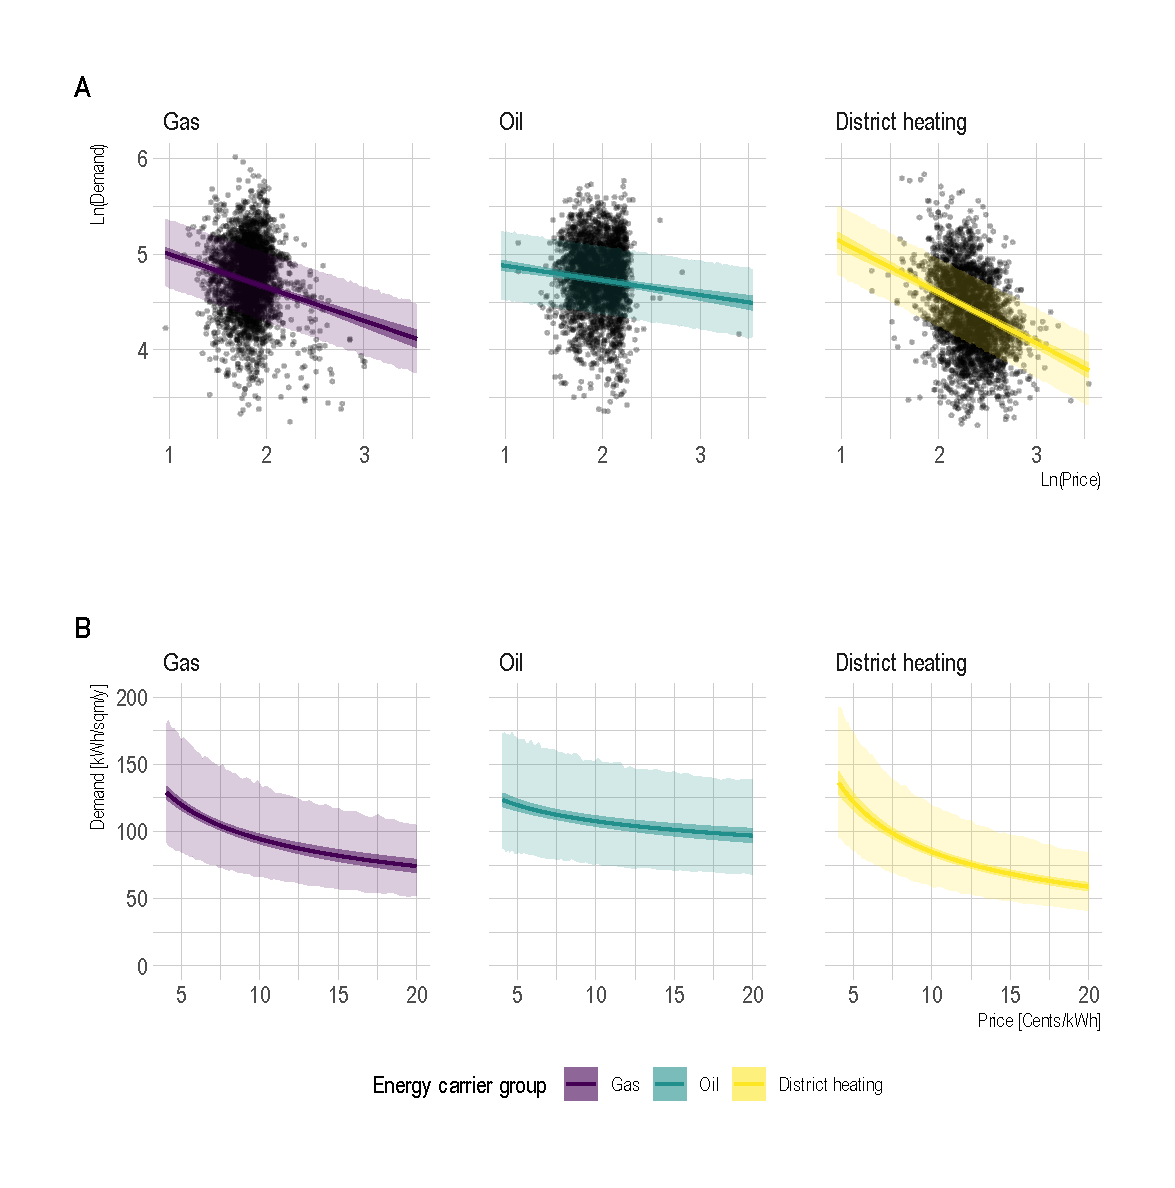
\includegraphics[width=1.04\linewidth]{figure/elasticity_predictions_subsample} 

}

\caption{Predicted price elasticities of demand by energy carrier group (bm.3)}\label{fig:elasticity-predictions-energy-carrier}
\end{figure}
\textbf{Model comparison}
\begin{table}[]
\centering
\caption{Model comparison based on PSIS-LOO}
\label{tab:model-comparison}
\begin{tabular}{@{}lrr@{}}
\toprule
     & \multicolumn{1}{l}{elpd\_diff} & \multicolumn{1}{l}{se\_diff} \\ \midrule
bm.3 & 0.0                            & 0.0                          \\
bm.2 & -14.7                          & 7.5                          \\
bm.1 & -90.3                          & 14.0                         \\
b.2  & -2856.7                        & 80.4                         \\
b.1  & -3100.5                        & 81.6                         \\ \bottomrule
\end{tabular}
\end{table}
\hypertarget{discussion}{%
\chapter{Discussion}\label{discussion}}

NOTES - Energy taxation and climate change:
- Fuel consumption demand is determined by demand functions that depend primarily on income and prices
- Those who disfavor fuel taxes often claim they are strongly regressive. Earlier studies have shown that this depends on the country studied and on the details of the methods used, for instance if lifetime or temporary income is used, if substitution or other reactions are allowed for in the analysis. There is a tendency to progressivity in low income countries but regressivity in high income countries.
- Indirect channel of long-term price change and anticipation of those changes leading to investments in low-carbon UBA: Remediation measures drawn by lot through the BEHG are partly subsidized through the BEG or the tax incentive and are accounted for there (CO2 price as door opener for subsidy)

\hypertarget{discussion-of-elasticity-results}{%
\section{Discussion of elasticity results}\label{discussion-of-elasticity-results}}

Relevante Stellen für Rückbezüge aus der Literatur:
\begin{itemize}
\item
  In their analysis, \protect\hyperlink{ref-labandeira_etal17}{Labandeira et al.} (\protect\hyperlink{ref-labandeira_etal17}{2017}) include a total of 428 papers, all published between 1990 and 2016. For the demand of natural gas, they find an average short-term (long-term) price elasticity of -0.18 (-0.57) based on 230 individual estimates. And for heating oil they find a comparable average short-term (long-term) elasticity of -0.19 (-0.54), which, however, is based on only 44 individual estimates (\protect\hyperlink{ref-labandeira_etal17}{Labandeira et al., 2017}). An average elasticity for space heating -- which is less focused on in the literature due to its relatively low prevalence -- is not provided.
\item
  There are three earlier studies that have a spatial focus on Germany. The first study was conducted by \protect\hyperlink{ref-rehdanz07}{Rehdanz} (\protect\hyperlink{ref-rehdanz07}{2007}), who estimates short-term price elasticities for different energy carrier groups for residential space heating demand. She uses social survey data on household-level heating expenditures from the Socio-Economic Panel (SOEP) in the years 1998 and 2003. Methodologically, a cross-sectional statistical analysis with dummy variables is conducted for the two years. In contrast to the meta-estimates presented in the previous part of the Chapter, the study finds that demand for heating oil is highly elastic with estimates ranging between -1.68 and -2.03, depending on the model specification. For gas, the results indicate an inelastic elastic demand between -0.44 and -0.63 (depending on the model specification) which is nevertheless significantly more elastic than the meta-estimates presented previously. Therefore, the study concludes that the type of energy carrier can have a strong influence on the price sensitivity of households (\protect\hyperlink{ref-rehdanz07}{Rehdanz, 2007}).
  \#\# The role of energy prices and interaction with complementary measures (policy-mix)
\item
  For district heating larger share of costs are fixed; may drive the effect of larger price elasticities as data does not differentiate between fixed and variable cost components and with lower energy demand the per-unit cost rate increses due to the larger
\item
  Prices not the only option for action, potential overestimation of price relevance
\item
  Warmmietenmodell (Now only the renters are effected which will mainly trigger short-term price reactions; for decarbonisation need to tap the long-term channel; Lessors must be incentivized to initialize efficiency measures; one option: split prices but then long-term price signal is still partly muted; Warmmietmodell as an alternative where both parties renters and lessors have full economic incentive of pricing measures)
\end{itemize}
Relevance of Policy Mix - UBA (2022) study:
\begin{itemize}
\item
  Simulate the effect of various price paths for the BEHG until 2030 and simulate for the buildings sector (also consider the transportation and industry sector) how those varying price paths affect the level of sectoral emissions.
\item
  Shortcoming: They do not consider demand effects from price changes --\textgreater{} short-term effects that this theses argues for; prices are only endogenous effects on the long-term investment desicions.
\item
  Additional Shortcoming: Simulate choice of heat supply system, but not additional renovations, for example of the building envelope
\item
  With the findings from this thesis it must therefore be assumed that actual emissions would be lower than simulated in the model not considering demand adjustments from higher energy prices
\item
  Three scenarios: 1. BaU CO2 price of 125€/t in 2030; 2. Foresight, anticipation of energy prices for coming 5/10 yrs; 3. Foresight AND shorter lifetimes of heating systems (75\% of usual life-time) for increased replacement.
\item
  BaU: 86 Mt CO2e in 2030, KSG 2021 sector goal for buildings: 67 Mt CO2e in 2030; 28.4\% above the target
\item
  Only the scenarios with adjusted replacement rates + foresight meet or fall below the KSG (2021) targets (amended 2021 version).
\item
  Anticipation of higher CO2 prices over long time span has high impact; but effect about three times as large when combined with shorter lifetimes of heating systems
\item
  In scenarios with the assumption that heat supply systems are replaced more quickly due to the rising CO2 price, the heating replacement rate increases to around 5\%. In sensitivities in which no shorter lifetimes of the heat supply systems are assumed, the heating replacement rate is significantly lower.
\item
  Investitionsentscheidungen sind bedarfsgetrieben --\textgreater{} Policy Mix kann hier abhilfe Schaffen (bonus-malus system)
\item
  Another key finding is that significantly greater savings can be achieved if the capital good is replaced before the end of its respective service life. Due to the long-term capital stocks, the effects are greatest in the buildings and industry sectors, while in the transport sector the additional effect of early replacement is limited due to the comparatively short holding periods of vehicles.
\item
  Zusammenspiel: nur wenn fossile Investitionsgüter wirtschaftlich unattraktiv sind, wird durch die Austauschratenerhöhung die gewünschte Wirkung erzielt. Zusätzloiche Maßnahmen könnten sein: Verbesserung von Informationsverfügbarkeit, Ordnungsrecht oder finanzielle Förderungen. Besondere Bedeutung ist dabei einem verlässlich kommunizierten Preispfad des BEHG zuzumessen.
\item
  Das im Rahmen der aktuellen Beratungen zum Fit-for-55-Paket der EU zu erwartende verschärfte, neue ESR-Ziel wie auch die daraus abgeleitete neue BEHG-Höchstmenge wird in keiner CO2-Preissensitivität eingehalten.--\textgreater{} Einhaltung der ambitionierteren BEHG-Ziele höhere CO2-Preise als hier analysiert zu erwarten sind bzw. darüberhinausgehende klimapolitische Instrumente erforderlich sind
\item
  Damit bestätigt sich mit dieser Modellierungsarbeit auch die wirtschaftstheoretische Herleitung (vgl. Kemfert et al.~(2021)), dass zur Erreichung der Klimaschutzziele ein Politik-Mix zielführend ist, welcher die CO2-Bepreisung mit ordnungsrechtlichen Instrumenten, Förderprogrammen und weiteren Instrumenten (z.B. dem Abbau klimaschädlicher Subventionen) kombiniert.
\end{itemize}
\hypertarget{conclusion}{%
\chapter{Conclusion}\label{conclusion}}

The elasticity estimates from this thesis may also be relevant for other countries and regions that have comparable conditions to Germany in terms of building stock and energy demand and also face the challenge of decarbonising the buildings sector in the coming decades. Here, my results would serve as an empirical guide to the short-term demand effects for any kind of price-related policy instrument.

\appendix

\hypertarget{supplementary-materials}{%
\chapter{Supplementary materials}\label{supplementary-materials}}

\singlespacing
\newpage
\begin{figure}

{\centering 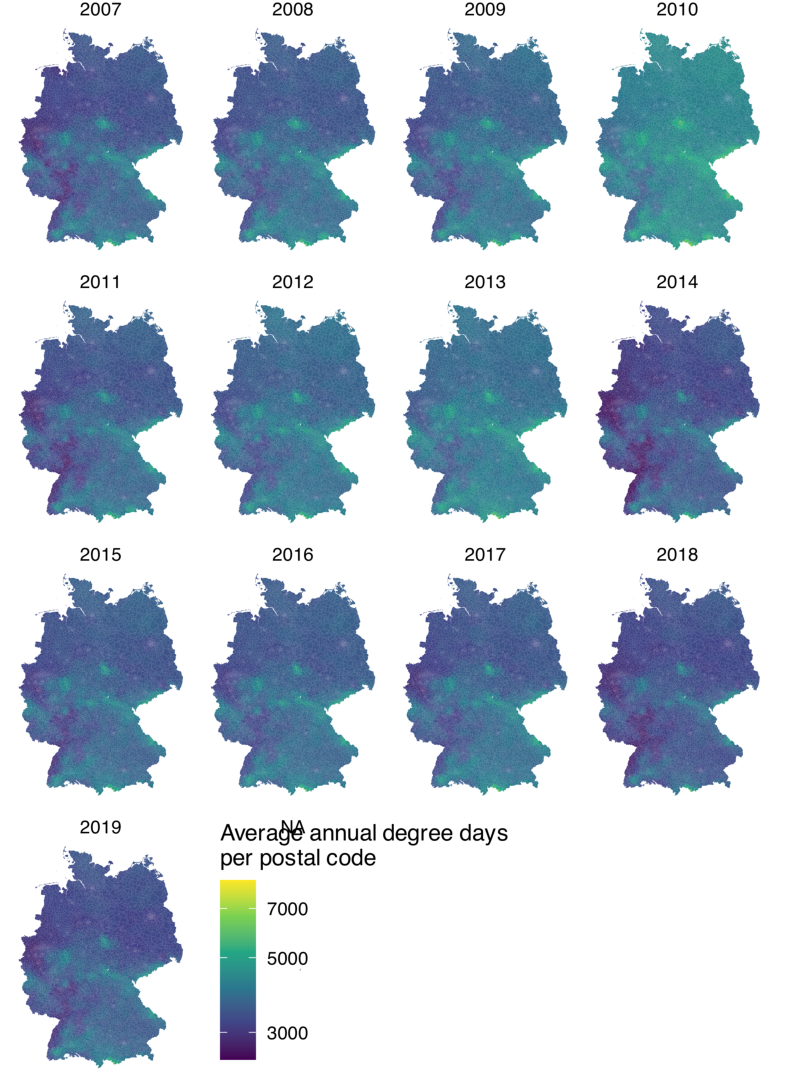
\includegraphics[width=0.77\linewidth]{figure/distribution_degree_days} 

}

\caption{Spatial and temporal variation in degree days}\label{fig:degree-days-distribution}
\end{figure}
\noindent
Figure \ref{fig:degree-days-distribution} show the spatial and temporal variation of outside temperature measured in degree days. Degree days data was taken from \protect\hyperlink{ref-iwu21}{IWU} (\protect\hyperlink{ref-iwu21}{2021}) and are used as an additional determinant of space heat demand in the regression analysis. Data is shown on the postal code level. Higher annual degree days are associated with lower temperatures and vice versa. In terms of spatial variation, the maps show cooler temperatures (higher degree days) mainly in the higher altitude regions, but also in eastern Germany, which is further inland from the European continent. In terms of temporal variation, 2010 in particular, but also 2012 and 2013 were cooler years than the average year in the sample. 2014, 2018 and 2019, on the other hand, were significantly warmer years.

\newpage
\begin{figure}

{\centering 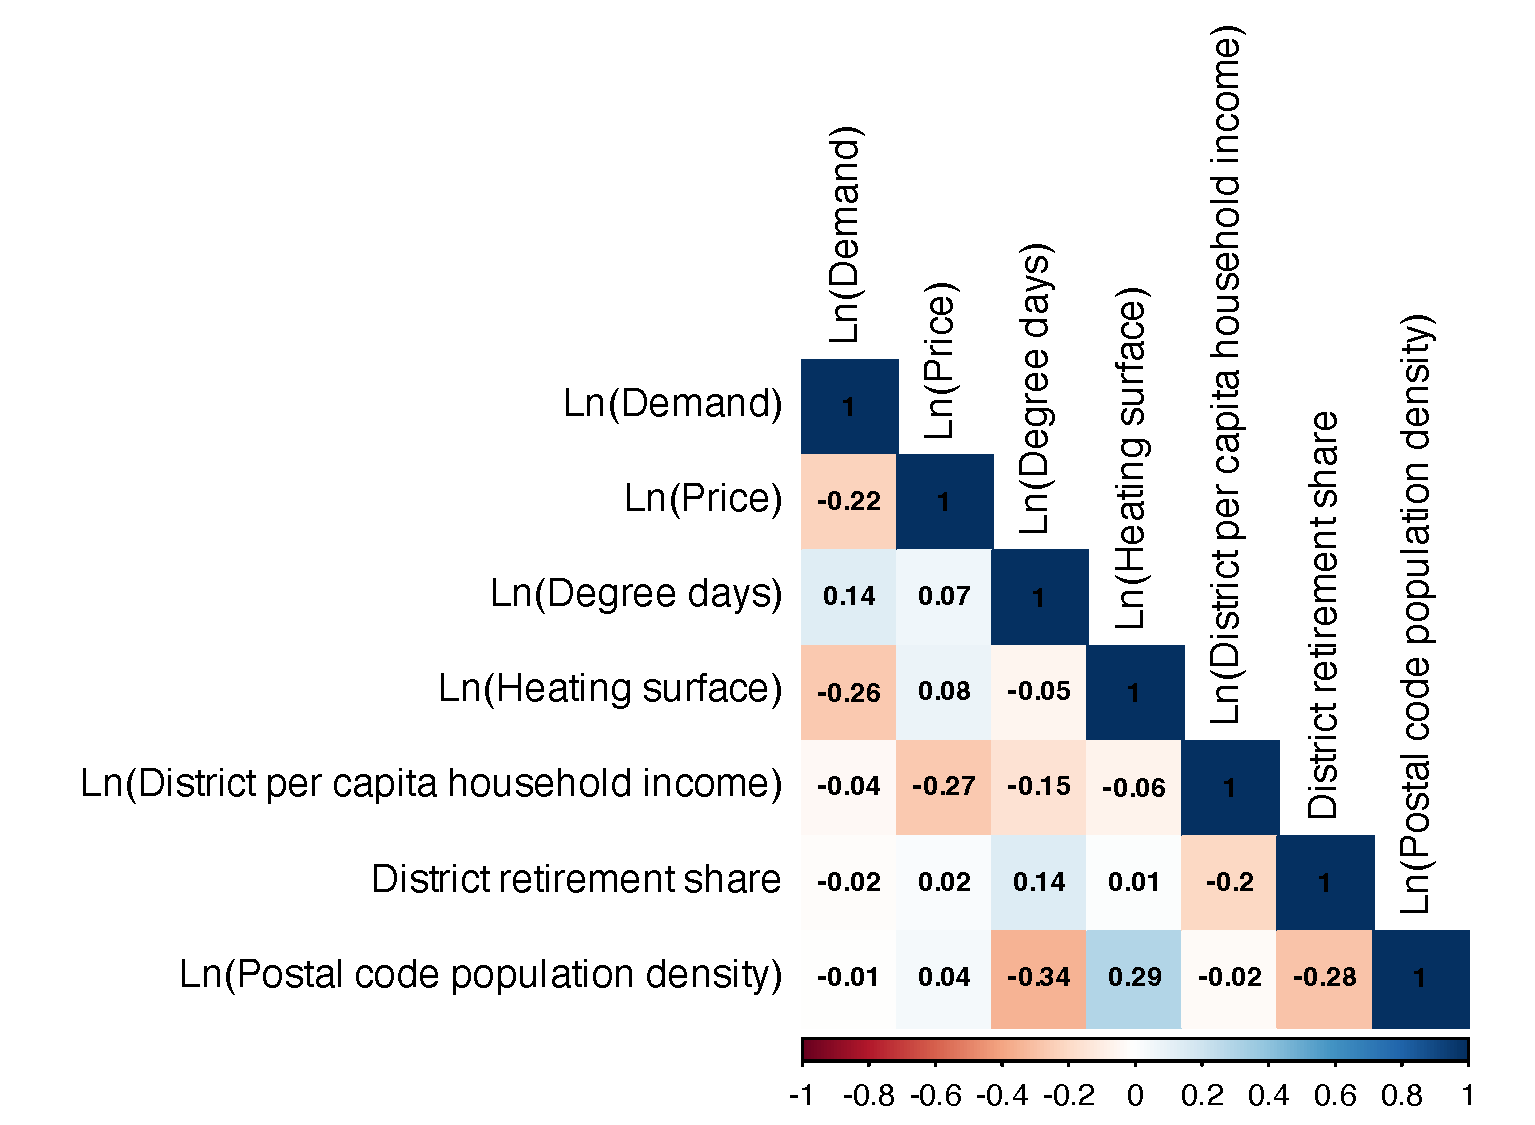
\includegraphics[width=0.9\linewidth]{figure/correlation_matrix} 

}

\caption{Pearson’s correlation matrix}\label{fig:correlation-plot}
\end{figure}
\noindent
The values in Figure \ref{fig:correlation-plot} represent Pearson's correlation coefficients. Values closer to 1 indicate a stronger positive relationship, values closer to -1 indicate a stronger negative relationship. Values close to zero indicate no relationship. None of the correlations observed between the variables exceed moderate values, ruling out possible multicollinearity issues. Energy price is negatively correlated with energy demand, indicating that the expected negative effect of price on demand indeed exists. Note that all variables except the district retirement share, which is already a ratio, are ln-transformed and reflect the data transformation used in the regression analysis.

\newpage
\begin{table}[]
\centering
\caption{Descriptive statistics for age of buildings and heating systems}
\label{tab:age-building-heating-system}
\resizebox{\textwidth}{!}{%
\begin{tabular}{@{}lllll@{}}
\toprule
Variable &
  \begin{tabular}[c]{@{}l@{}}Overall\\ N = 2,718,246\end{tabular} &
  \begin{tabular}[c]{@{}l@{}}Gas\\ N = 1,647,563\end{tabular} &
  \begin{tabular}[c]{@{}l@{}}Oil\\ N = 802,451\end{tabular} &
  \begin{tabular}[c]{@{}l@{}}District heating\\ N = 268,232\end{tabular} \\ \midrule
                                      &                    &                 &               &               \\
{\ul Building construction year}      &                    &                 &               &               \\
Until 1918                            & 34,536 (9.5\%)     & 22,004 (10.0\%) & 6,622 (6.1\%) & 5,910 (17\%)  \\
1919-1948                             & 22,652 (6.2\%)     & 14,494 (6.6\%)  & 4,742 (4.3\%) & 3,416 (9.7\%) \\
1949-1978                             & 121,949 (33\%)     & 68,253 (31\%)   & 42,973 (39\%) & 10,723 (30\%) \\
1979-1995                             & 126,299 (35\%)     & 76,869 (35\%)   & 40,072 (37\%) & 9,358 (26\%)  \\
1996-2009                             & 58,582 (16\%)      & 38,409 (17\%)   & 14,411 (13\%) & 5,762 (16\%)  \\
After 2010                            & 1,172 (0.3\%)      & 738 (0.3\%)     & 288 (0.3\%)   & 146 (0.4\%)   \\
(Missing)                             & 2,353,056          & 1,426,796       & 693,343       & 232,917       \\
                                      &                    &                 &               &               \\
\multicolumn{2}{l}{{\ul Heating system installation year}} &                 &               &               \\
Until 1978                            & 11,486 (3.5\%)     & 6,360 (3.2\%)   & 4,296 (4.5\%) & 830 (2.6\%)   \\
1979-1995                             & 118,401 (36\%)     & 71,848 (36\%)   & 36,359 (38\%) & 10,194 (32\%) \\
1996-2009                             & 151,172 (46\%)     & 93,734 (47\%)   & 41,161 (43\%) & 16,277 (51\%) \\
After 2010                            & 46,556 (14\%)      & 27,564 (14\%)   & 14,532 (15\%) & 4,460 (14\%)  \\
(Missing)                             & 2,390,631          & 1,448,057       & 706,103       & 236,471       \\
                                      &                    &                 &               &               \\ \midrule
\textit{Note: n (\%)}                 &                    &                 &               &               \\ \bottomrule
\end{tabular}%
}
\end{table}
\noindent
Table \ref{tab:age-building-heating-system} provides descriptive statistics for the age of buildings and heating systems grouped by the type of energy carrier. For those buildings, where information is available, a relatively larger share of district heating systems are installed in older buildings but at a more recent date. Overall, however, the differences are moderate and cannot explain the difference in energy demand between buildings with gas and oil heating on the one side (relatively higher consumption) and district heating on the other side (relatively lower consumption). Instead, it is presumably the size of the buildings that induces to the lower demand levels for buildings with district heating (cf.~Table \ref{tab:summary-statistics}. At the same time, it should be noted that the validity of the age classification of buildings and heating system installation year presented here is limited, as the information is available only for 15.5\% and 13.7\% of the total number of observations, respectively. This is also the reason why the two variables were not included as variables in the regression analysis.

\newpage
\begin{figure}

{\centering 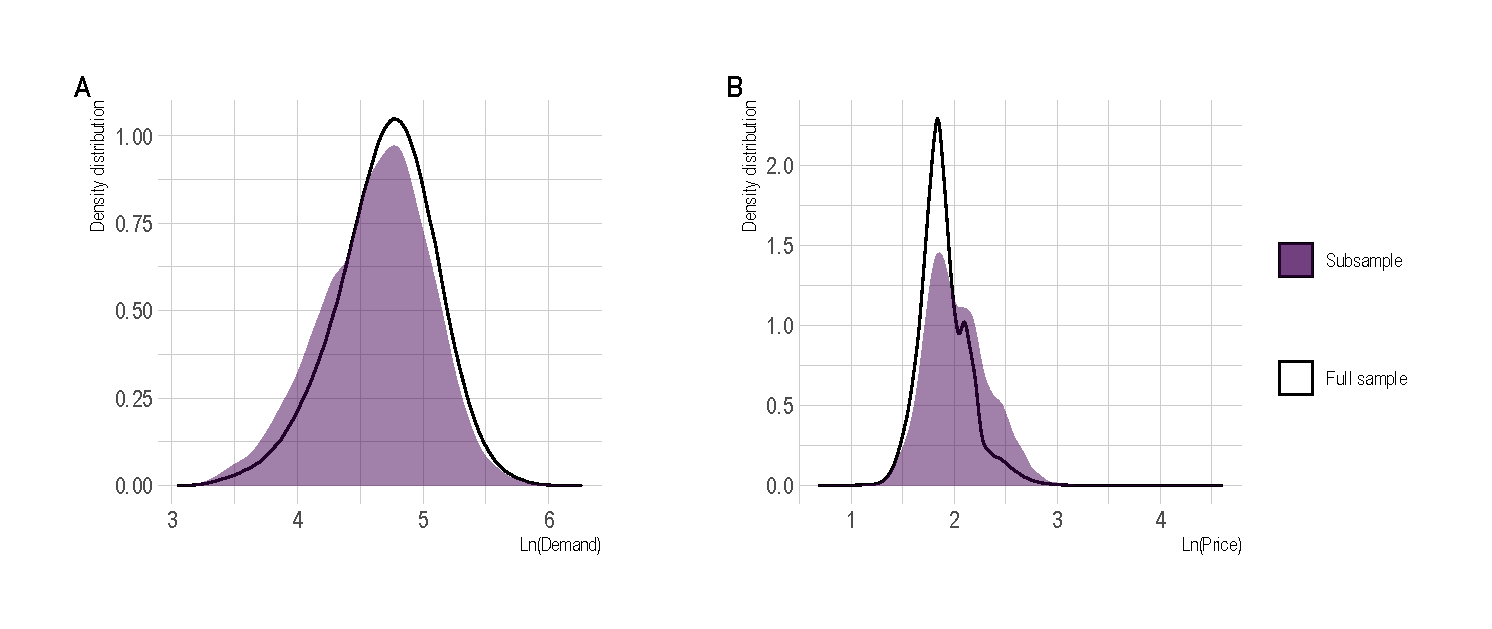
\includegraphics[width=1\linewidth]{figure/density-distribution-comparison-samples} 

}

\caption{Comparison of density distribution for energy demand and price between full sample and subsample}\label{fig:density-distribution-comparison-samples}
\end{figure}
\noindent
Figure \ref{fig:density-distribution-comparison-samples} compares the density distribution for the two key variables energy demand and energy price between the full sample (transparent) and the subsample (purple area) with 400 randomly selected buildings per energy carrier group (gas, oil and district heating). The visual comparison shows that there are only relatively small deviations in energy demand (Panel A), with the distribution in the subsample being slightly shifted to the left (lower demand). The comparison of distribution in energy prices (Panel B), on the other hand, show more divergence, with the subsample distribution showing a lower peak around \(Ln(price) = 2\) and also more observations in the higher price range. However, the deviations in energy demand and energy prices can be well explained by the stratified sampling approach for the subsample. The stratified sample leads primarily to a reduction in the share of gas observations and in contrast to an increase in observations related to district heating. For the demand variable, more district heating observations lead to more observations with a lower demand. For the price variable, it leads to a less pronounced peak in gas observations at the center and more district heating observations with higher prices at the upper end of the distribution.

\newpage

\tiny
\begin{longtable}[c]{lrrrrrrr}
\caption{Full model results for subsample analysis}
\label{tab:brms-full-model-results}\\
\cline{2-8}
 & \multicolumn{1}{c}{\textbf{Estimate}} & \multicolumn{1}{c}{\textbf{Est.Error}} & \multicolumn{1}{c}{\textbf{l-95\% CI}} & \multicolumn{1}{c}{\textbf{u-95\% CI}} & \multicolumn{1}{c}{\textbf{Rhat}} & \multicolumn{1}{c}{\textbf{Bulk ESS}} & \multicolumn{1}{c}{\textbf{Tail ESS}} \\ \cline{2-8} 
\endfirsthead
%
\endhead
%
\hline
\endfoot
%
\endlastfoot
%
 &  &  &  &  &  &  &  \\ \hline
\textbf{B.1} &  &  &  &  &  &  &  \\
{\ul \textit{Population-Level-Effects:}} &  &  &  &  &  &  &  \\
Intercept & 5.75 & 0.03 & 5.69 & 5.82 & 1.00 & 3240 & 2312 \\
ln(Price) & -0.56 & 0.01 & -0.59 & -0.53 & 1.00 & 3240 & 2432 \\ \hline
 &  &  &  &  &  &  &  \\ \hline
\textbf{B.2} &  &  &  &  &  &  &  \\
{\ul \textit{Population-Level-Effects:}} &  &  &  &  &  &  &  \\
Intercept & 4.93 & 0.49 & 3.94 & 5.89 & 1.00 & 3423 & 2799 \\
ln(Price) & -0.41 & 0.02 & -0.45 & -0.38 & 1.00 & 2740 & 2644 \\
ln(Degree.days) & 0.57 & 0.04 & 0.50 & 0.65 & 1.00 & 4404 & 2986 \\
ln(Heating.surface) & -0.15 & 0.01 & -0.16 & -0.14 & 1.00 & 3662 & 3067 \\
Carrier.group.oil & 0.04 & 0.01 & 0.02 & 0.06 & 1.00 & 3633 & 2650 \\
Carrier.group.district.heating & -0.06 & 0.01 & -0.09 & -0.03 & 1.00 & 2588 & 2890 \\
ln(District.income) & -0.35 & 0.03 & -0.41 & -0.29 & 1.00 & 4126 & 2746 \\
ln(Pop.density) & 0.05 & 0.00 & 0.04 & 0.05 & 1.00 & 3955 & 3125 \\
District.retire & -0.05 & 0.17 & -0.37 & 0.28 & 1.00 & 4222 & 3258 \\ \hline
 &  &  &  &  &  &  &  \\ \hline
\textbf{BM.1} &  &  &  &  &  &  &  \\
{\ul \textit{Population-Level-Effects:}} &  &  &  &  &  &  &  \\
Intercept & 5.31 & 0.04 & 5.23 & 5.39 & 1.00 & 1141 & 1800 \\
ln(Price) & -0.33 & 0.02 & -0.36 & -0.30 & 1.00 & 1565 & 1970 \\
 &  &  &  &  &  &  &  \\
{\ul \textit{Group-Level-Effects:}} &  &  &  &  &  &  &  \\
$\sim$id (Number of levels: 1200) &  &  &  &  &  &  &  \\
sd(Intercept) & 0.36 & 0.01 & 0.34 & 0.37 & 1.00 & 482 & 990 \\
 &  &  &  &  &  &  &  \\
$\sim$year (Number of levels: 13) &  &  &  &  &  &  &  \\
sd(Intercept) & 0.09 & 0.02 & 0.06 & 0.14 & 1.01 & 745 & 1844 \\ \hline
 &  &  &  &  &  &  &  \\ \hline
\textbf{BM.2} &  &  &  &  &  &  &  \\
{\ul \textit{Population-Level-Effects:}} &  &  &  &  &  &  &  \\
Intercept & 1.65 & 0.77 & 0.12 & 3.14 & 1.01 & 471 & 1247 \\
ln(Price) & -0.30 & 0.02 & -0.33 & -0.27 & 1.00 & 2318 & 2796 \\
ln(Degree.days) & 0.69 & 0.05 & 0.60 & 0.79 & 1.00 & 1378 & 1915 \\
Carrier.group.oil & 0.06 & 0.02 & 0.02 & 0.10 & 1.01 & 443 & 1067 \\
Carrier.group.district.heating & -0.12 & 0.02 & -0.16 & -0.08 & 1.02 & 401 & 930 \\
ln(District.income) & -0.20 & 0.06 & -0.32 & -0.08 & 1.01 & 364 & 934 \\
District.retire & -0.18 & 0.25 & -0.67 & 0.30 & 1.01 & 660 & 1176 \\
 &  &  &  &  &  &  &  \\
{\ul \textit{Group-Level-Effects:}} &  &  &  &  &  &  &  \\
$\sim$id (Number of levels: 1200) &  &  &  &  &  &  &  \\
sd(Intercept) & 0.35 & 0.01 & 0.34 & 0.37 & 1.01 & 461 & 855 \\
 &  &  &  &  &  &  &  \\
$\sim$year (Number of levels: 13) &  &  &  &  &  &  &  \\
sd(Intercept) & 0.03 & 0.01 & 0.02 & 0.05 & 1.00 & 1013 & 1516 \\ \hline
 &  &  &  &  &  &  &  \\ \hline
\textbf{BM.2 Lagged} &  &  &  &  &  &  &  \\
{\ul \textit{Population-Level-Effects:}} &  &  &  &  &  &  &  \\
Intercept & 0.88 & 0.92 & -0.97 & 2.70 & 1.01 & 532 & 975 \\
ln(Price, lagged t-1) & -0.16 & 0.02 & -0.20 & -0.12 & 1.00 & 2254 & 2452 \\
ln(Degree.days) & 0.72 & 0.06 & 0.60 & 0.83 & 1.01 & 1251 & 1975 \\
Carrier.group.oil & 0.04 & 0.02 & 0.00 & 0.09 & 1.01 & 364 & 617 \\
Carrier.group.district.heating & -0.20 & 0.02 & -0.25 & -0.16 & 1.00 & 460 & 903 \\
ln(District.income) & -0.17 & 0.07 & -0.31 & -0.03 & 1.01 & 455 & 963 \\
District.retire & -0.33 & 0.28 & -0.86 & 0.22 & 1.00 & 586 & 1219 \\
 &  &  &  &  &  &  &  \\
{\ul \textit{Group-Level-Effects:}} &  &  &  &  &  &  &  \\
$\sim$id (Number of levels: 1164) &  &  &  &  &  &  &  \\
sd(Intercept) & 0.36 & 0.01 & 0.34 & 0.37 & 1.00 & 506 & 866 \\
 &  &  &  &  &  &  &  \\
$\sim$year (Number of levels: 11) &  &  &  &  &  &  &  \\
sd(Intercept) & 0.03 & 0.01 & 0.02 & 0.05 & 1.00 & 1116 & 1753 \\ \hline
 &  &  &  &  &  &  &  \\ \hline
\textbf{BM.3} &  &  &  &  &  &  &  \\
{\ul \textit{Population-Level-Effects:}} &  &  &  &  &  &  &  \\
Intercept & 2.13 & 0.77 & 0.65 & 3.71 & 1.01 & 557 & 1248 \\
ln(Price) & -0.35 & 0.03 & -0.40 & -0.29 & 1.00 & 1309 & 2241 \\
ln(Degree.days) & 0.68 & 0.05 & 0.58 & 0.78 & 1.01 & 1106 & 1872 \\
Carrier.group.oil & -0.32 & 0.06 & -0.44 & -0.19 & 1.01 & 1175 & 2149 \\
Carrier.group.district.heating & 0.31 & 0.08 & 0.15 & 0.46 & 1.00 & 1139 & 1866 \\
ln(District.income) & -0.23 & 0.06 & -0.35 & -0.12 & 1.02 & 426 & 651 \\
District.retire & -0.18 & 0.27 & -0.71 & 0.34 & 1.01 & 370 & 924 \\
ln(Price):Carrier.group.oil & 0.19 & 0.03 & 0.13 & 0.26 & 1.00 & 1441 & 2276 \\
ln(Price):Carrier.group.district.heating & -0.18 & 0.04 & -0.25 & -0.11 & 1.00 & 1202 & 2009 \\
 &  &  &  &  &  &  &  \\
{\ul \textit{Group-Level-Effects:}} &  &  &  &  &  &  &  \\
$\sim$id (Number of levels: 1200) &  &  &  &  &  &  &  \\
sd(Intercept) & 0.35 & 0.01 & 0.33 & 0.36 & 1.01 & 386 & 687 \\
 &  &  &  &  &  &  &  \\
$\sim$year (Number of levels: 13) &  &  &  &  &  &  &  \\
sd(Intercept) & 0.03 & 0.01 & 0.01 & 0.04 & 1.00 & 912 & 1752 \\ \hline
\end{longtable}
\normalsize

\noindent
Table \ref{tab:brms-full-model-results} presents the complete model summaries for the brms models in the subsample analysis. The parameters are summarized using either the mean (estimate) or the standard deviation (standard error) of the posterior distribution with 95\% confidence intervals. Rhat is a measure of model convergence. Values below 1.05 indicate that chains mixed well and the model has converged. Bulk ESS and Tail ESS are diagnostics of the sampling efficiency.

\newpage
\begin{figure}

{\centering 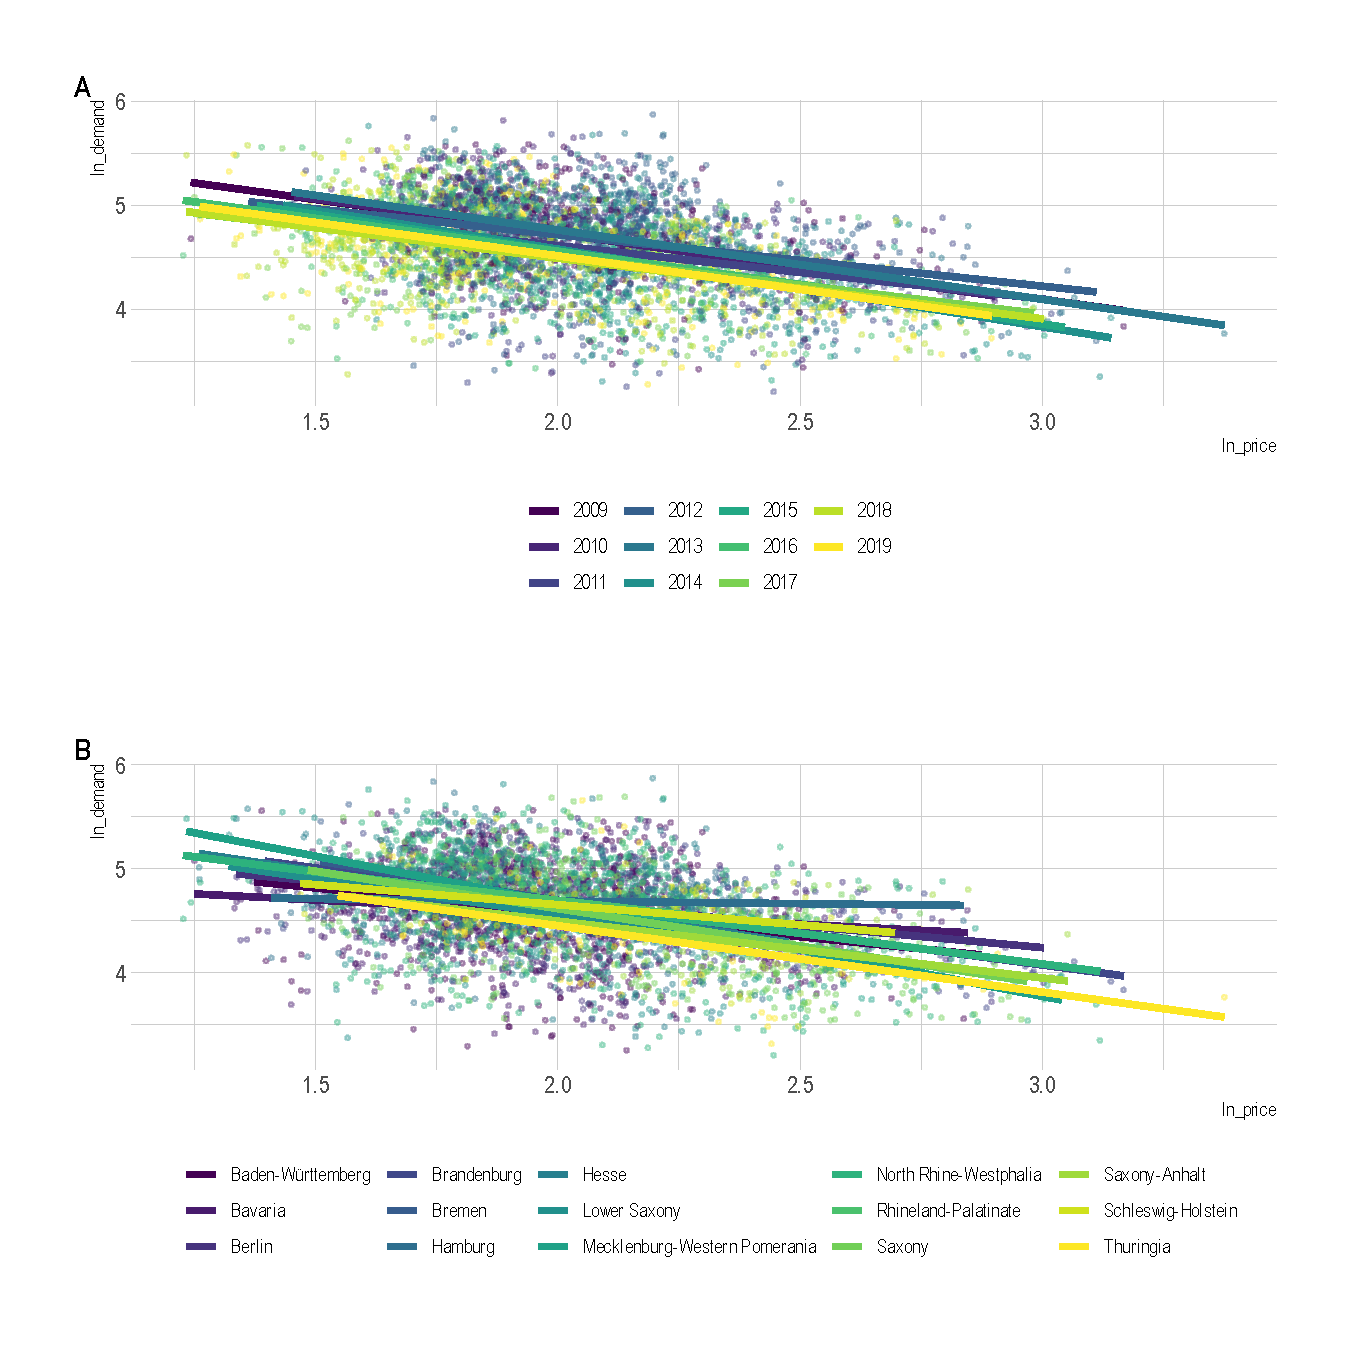
\includegraphics[width=1\linewidth]{figure/year_state_heterogeneity_plot} 

}

\caption{Investigation of heterogeneity for years and federal states}\label{fig:heterogeneity-year-state-plot}
\end{figure}
\noindent
Figure \ref{fig:heterogeneity-year-state-plot} presents a visual examination of the heterogeneity of price elasticity between years (Panel A) and federal states (Panel B). For this purpose, the observations in the sub-sample are grouped by year/federal state and presented in a scatter plot. The lines in the diagrams reflect simple linear models for the years/federal states as groups. Between years, all lines are almost parallel, indicating that there is no relevant difference in price elasticity between years. For the federal states, the lines scatter a little. At the same time, however, no strong pattern can be discerned through clusters such as differences between formerly eastern and western federal states or through other regional clusters.

\newpage
\begin{figure}

{\centering 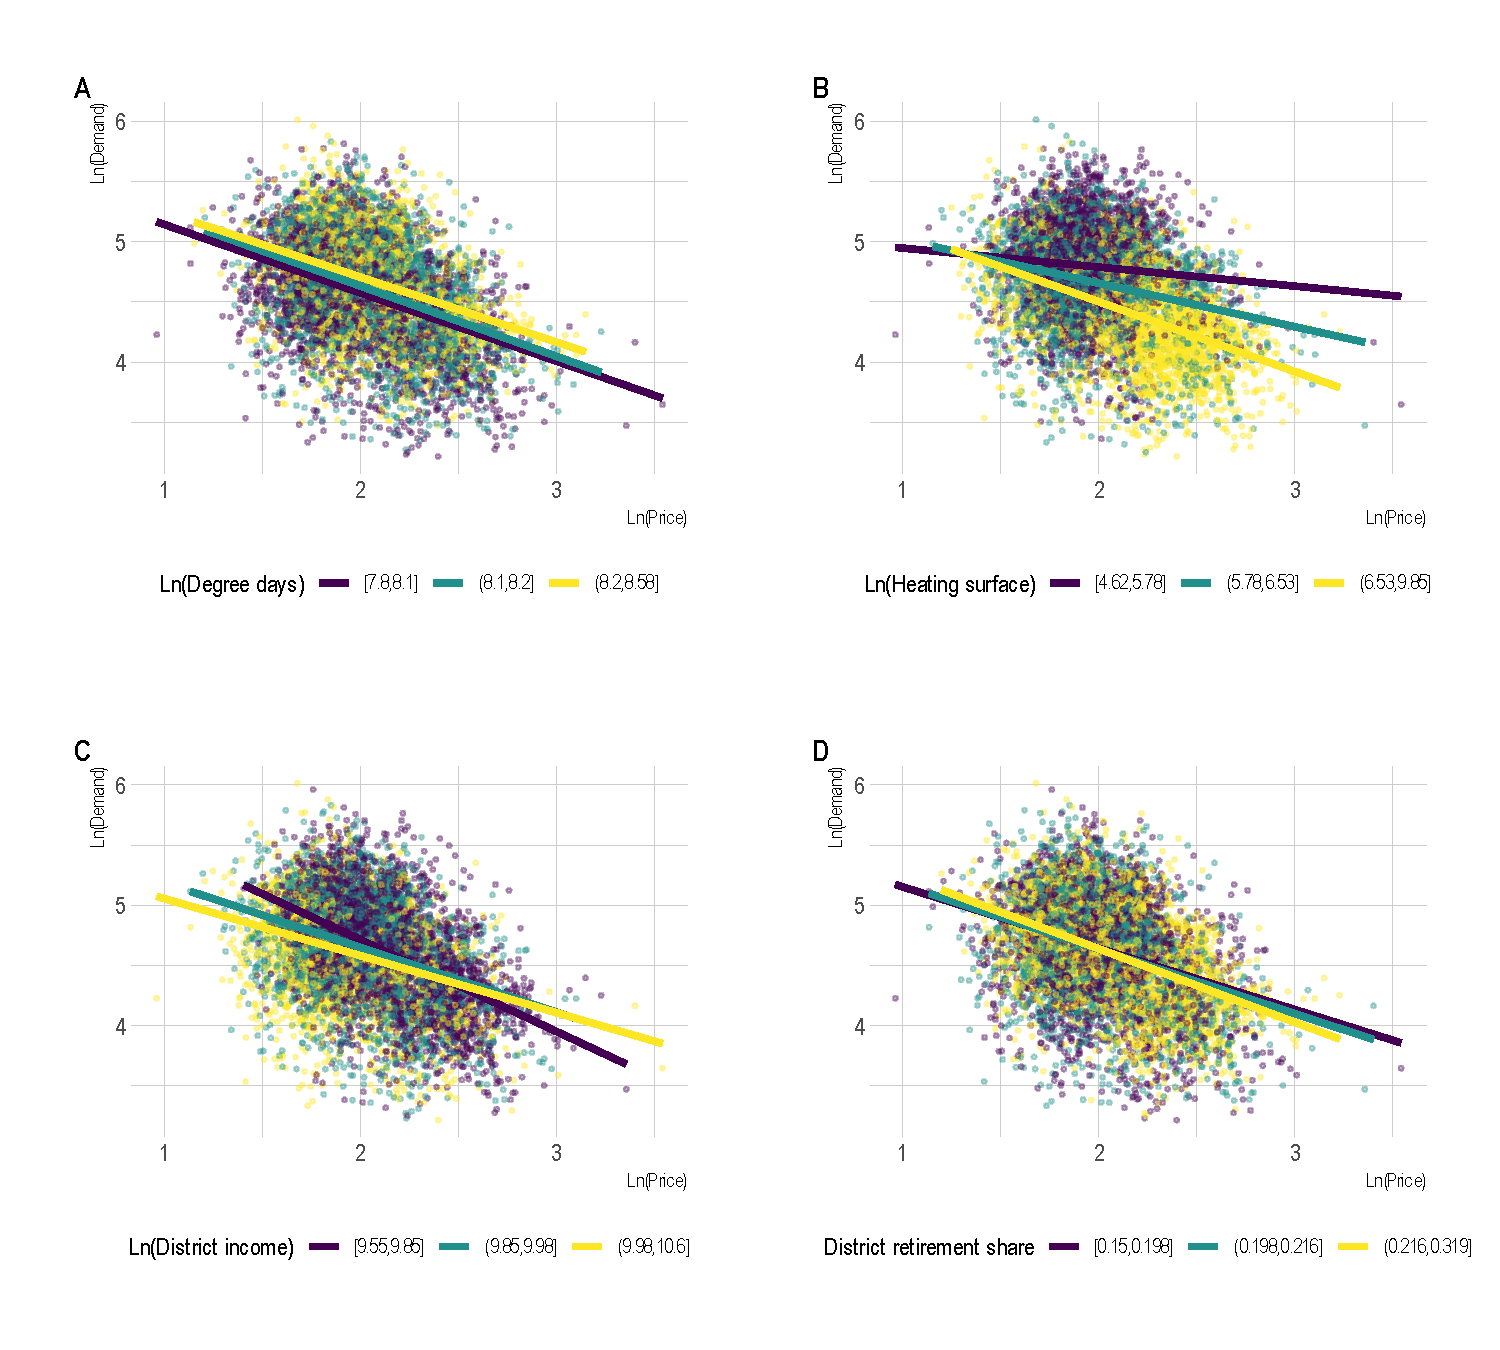
\includegraphics[width=0.95\linewidth]{figure/other_variables_heterogeneity_plot} 

}

\caption{Investigation of heterogeneity for degree days, heating surface, district income, and district retirement share}\label{fig:other-variables-heterogeneity-plot}
\end{figure}
\noindent
Figure \ref{fig:other-variables-heterogeneity-plot} presents a visual examination of the heterogeneity of price elasticity for the four variables degree days (Panel A), building heating surface (Panel B), average district income (Panel C), and district retirement share (Panel D). Since all four variables represent continuous variables, observations in the sub-sample are ln-transformed, grouped into three equally sized groups,\footnote{E.g., one third of observations with lowest number of degree days (between 7.85 and 8.1), one third of observations medium number of degree days (between 8.1 and 8.2), and one third of observations highest number of degree days (between 8.2 and 8.63).} and presented in a scatter plot. The lines in the diagrams reflect simple linear models for the respective three groups of equal size. For degree days, the lines are almost parallel and show no difference in price elasticity. For the other three variables, a slight dispersion of the grouped lines can be observed. But again, there are no pronounced differences that would prompt a more detailed investigation.

\newpage
\begin{figure}

{\centering 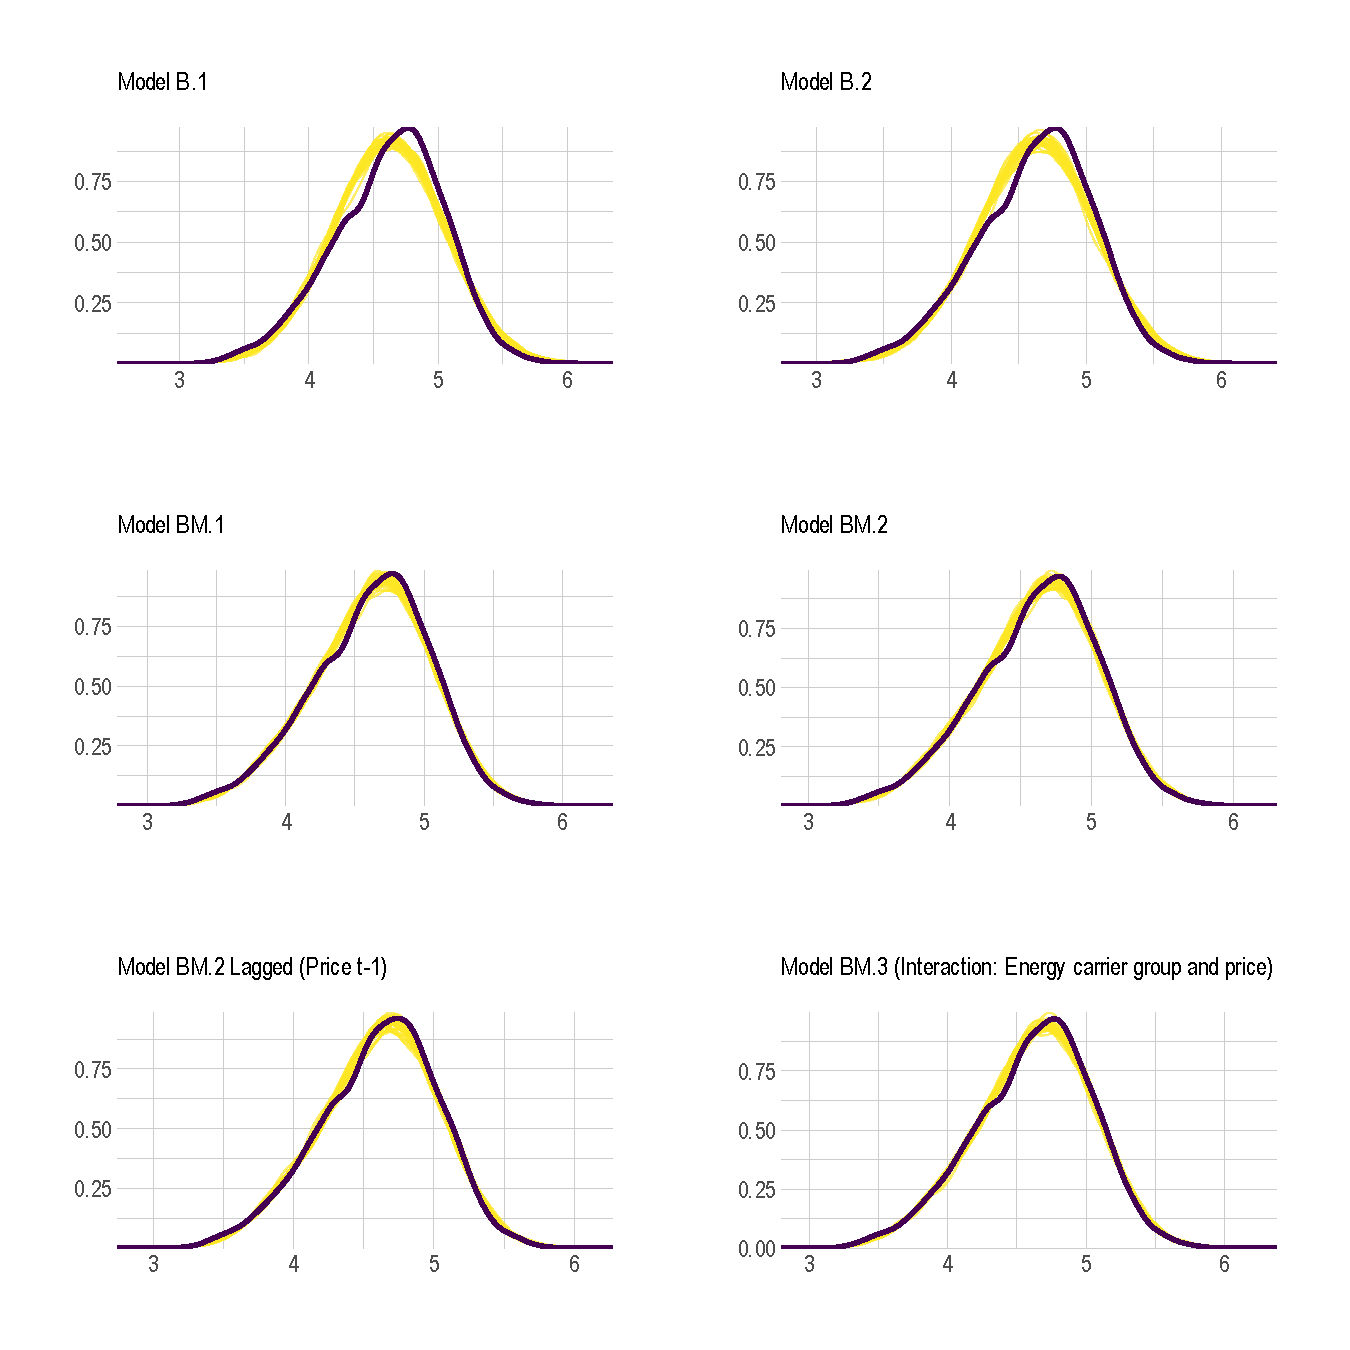
\includegraphics[width=1\linewidth]{figure/plot-model-comparison} 

}

\caption{Graphical model comparison for subsample analysis}\label{fig:plot-model-comparison}
\end{figure}
\noindent
Figure \ref{fig:plot-model-comparison} presents a visual examination of the model fit for all models used on the subsample analysis.

\newpage

\onehalfspacing

\hypertarget{declaration-of-authorship-eigenstuxe4ndigkeitserkluxe4rung}{%
\chapter*{Declaration of Authorship (Eigenständigkeitserklärung)}\label{declaration-of-authorship-eigenstuxe4ndigkeitserkluxe4rung}}
\addcontentsline{toc}{chapter}{Declaration of Authorship (Eigenständigkeitserklärung)}

Hiermit erkläre ich, dass ich die vorliegende Arbeit selbständig verfasst habe und sämtliche Quellen, einschließlich Internetquellen, die unverändert oder abgewandelt wiedergegeben werden, insbesondere Quellen für Texte, Grafiken, Tabellen und Bilder, als solche kenntlich gemacht habe.

Ich versichere, dass ich die vorliegende Abschlussarbeit noch nicht für andere Prüfungen eingereicht habe.

Mir ist bekannt, dass bei Verstößen gegen diese Grundsätze ein Verfahren wegen Täuschungsversuchs bzw. Täuschung gemäß der fachspezifischen Prüfungsordnung und/oder der Fächerübergreifenden Satzung zur Regelung von Zulassung, Studium und Prüfung der Humboldt-Universität zu Berlin (ZSP-HU) eingeleitet wird.

\hfill\break
~

\hfill\break
~

\hfill\break
~
\begin{tabular}{m{6cm}m{2cm}m{6cm}}
Berlin, den 04. August 2022 &  &              \\ \cline{1-1} \cline{3-3} 
\textit{Ort, Datum}            &  & \textit{Unterschrift} \\
                       &  &              \\
                       &  &             
\end{tabular}
\backmatter

\hypertarget{references}{%
\chapter*{References}\label{references}}
\addcontentsline{toc}{chapter}{References}

\markboth{References}{References}

\noindent

\setlength{\parindent}{-0.20in}

\hypertarget{refs}{}
\begin{CSLReferences}{1}{0}
\leavevmode\vadjust pre{\hypertarget{ref-ageb21}{}}%
AGEB. (2021). \emph{Auswertungstabellen zur Energiebilanz 1990 bis 2020}. Berlin. Retrieved from \url{https://ag-energiebilanzen.de/daten-und-fakten/auswertungstabellen/}

\leavevmode\vadjust pre{\hypertarget{ref-alberini_etal11}{}}%
Alberini, A., Gans, W., \& Velez-Lopez, D. (2011). Residential consumption of gas and electricity in the U.S.: The role of prices and income. \emph{Energy Economics}, \emph{33}(5), 870--881. http://doi.org/\href{https://doi.org/10.1016/j.eneco.2011.01.015}{10.1016/j.eneco.2011.01.015}

\leavevmode\vadjust pre{\hypertarget{ref-aldy_etal10}{}}%
Aldy, J. E., Krupnick, A. J., Newell, R. G., Parry, I. W. H., \& Pizer, W. A. (2010). Designing Climate Mitigation Policy. \emph{Journal of Economic Literature}, \emph{48}(4), 903--934. http://doi.org/\href{https://doi.org/10.1257/jel.48.4.903}{10.1257/jel.48.4.903}

\leavevmode\vadjust pre{\hypertarget{ref-auffhammer_rubin18}{}}%
Auffhammer, M., \& Rubin, E. (2018). \emph{Natural Gas Price Elasticities and Optimal Cost Recovery Under Consumer Heterogeneity: Evidence from 300 million natural gas bills} (No. w24295) (p. w24295). Cambridge, MA: National Bureau of Economic Research. Retrieved from \url{http://www.nber.org/papers/w24295.pdf}

\leavevmode\vadjust pre{\hypertarget{ref-bailey17}{}}%
Bailey, M. A. (2017). \emph{Real econometrics: The right tools to answer important questions}. New York: Oxford University Press.

\leavevmode\vadjust pre{\hypertarget{ref-bmwi21}{}}%
BMWi. (2021). \emph{Gesamtausgabe der Energiedaten}. BMWi. Retrieved from \url{https://www.bmwi.de/Redaktion/DE/Binaer/Energiedaten/energiedaten-gesamt-xls.xlsx?__blob=publicationFile\&v=133}

\leavevmode\vadjust pre{\hypertarget{ref-braungardt_etal21}{}}%
Braungardt, S., Bürger, V., \& Köhler, B. (2021). Carbon Pricing and Complementary Policies---Consistency of the Policy Mix for Decarbonizing Buildings in Germany. \emph{Energies}, \emph{14}(21), 7143. http://doi.org/\href{https://doi.org/10.3390/en14217143}{10.3390/en14217143}

\leavevmode\vadjust pre{\hypertarget{ref-brons_etal08}{}}%
Brons, M., Nijkamp, P., Pels, E., \& Rietveld, P. (2008). A meta-analysis of the price elasticity of gasoline demand. A SUR approach. \emph{Energy Economics}, \emph{30}(5), 2105--2122. http://doi.org/\href{https://doi.org/10.1016/j.eneco.2007.08.004}{10.1016/j.eneco.2007.08.004}

\leavevmode\vadjust pre{\hypertarget{ref-burger_etal19}{}}%
Bürger, V., Hesse, T., Köhler, B., Palzer, A., \& Engelmann, P. (2019). German Energiewende---different visions for a (nearly) climate neutral building sector in 2050. \emph{Energy Efficiency}, \emph{12}(1), 73--87. http://doi.org/\href{https://doi.org/10.1007/s12053-018-9660-6}{10.1007/s12053-018-9660-6}

\leavevmode\vadjust pre{\hypertarget{ref-burkner17}{}}%
Bürkner, P.-C. (2017). brms: An R package for Bayesian multilevel models using Stan. \emph{Journal of Statistical Software}, \emph{80}(1), 1--28. http://doi.org/\href{https://doi.org/10.18637/jss.v080.i01}{10.18637/jss.v080.i01}

\leavevmode\vadjust pre{\hypertarget{ref-csereklyei20}{}}%
Csereklyei, Z. (2020). Price and income elasticities of residential and industrial electricity demand in the European Union. \emph{Energy Policy}, \emph{137}, 111079. http://doi.org/\href{https://doi.org/10.1016/j.enpol.2019.111079}{10.1016/j.enpol.2019.111079}

\leavevmode\vadjust pre{\hypertarget{ref-cutler41}{}}%
Cutler, H. A. (1941). The Elasticity of the Residential Demand for Electricity. \emph{The Journal of Land \& Public Utility Economics}, \emph{17}(2), 242--245. http://doi.org/\href{https://doi.org/10.2307/3158428}{10.2307/3158428}

\leavevmode\vadjust pre{\hypertarget{ref-destatis18}{}}%
DESTATIS. (2018). Fernwärmeversorgung 2017: Abgegebene Wärmemenge leicht gesunken. Retrieved January 19, 2022, from \url{https://www.destatis.de/DE/Presse/Pressemitteilungen/2018/11/PD18_434_434.html}

\leavevmode\vadjust pre{\hypertarget{ref-destatis21c}{}}%
DESTATIS. (2021a). Bevölkerung: Kreise, Stichtag, Altersgruppen (12411-0017) {[}Text{]}. Retrieved January 22, 2022, from \url{https://www-genesis.destatis.de/genesis/online?operation=previous\&levelindex=0\&step=0\&titel=Tabellenaufbau\&levelid=1642855066461\&acceptscookies=false\#abreadcrumb}

\leavevmode\vadjust pre{\hypertarget{ref-destatis21}{}}%
DESTATIS. (2021b, November 12). Verbraucherpreisindex: Deutschland, Jahre (61111-0001). Retrieved November 12, 2021, from \url{https://www-genesis.destatis.de/genesis//online?operation=table\&code=61111-0001\&bypass=true\&levelindex=1\&levelid=1636748679996\#abreadcrumb}

\leavevmode\vadjust pre{\hypertarget{ref-erk20}{}}%
ERK. (2020). \emph{Bericht zur Vorjahresschätzung der deutschen Treibhausgasemissionen für das Jahr 2020}. Retrieved from \url{https://expertenrat-klima.de/content/uploads/2021/04/210415_Bericht_Expertenrat_Klimafragen_2021-2.pdf}

\leavevmode\vadjust pre{\hypertarget{ref-europeancomission19}{}}%
European Comission. (2019). \emph{The European Green Deal} (No. COM(2019) 640 final). Brussels. Retrieved from \url{https://eur-lex.europa.eu/legal-content/EN/TXT/HTML/?uri=CELEX:52019DC0640\&from=EN}

\leavevmode\vadjust pre{\hypertarget{ref-gaure2013lfe}{}}%
Gaure, S. (2013). lfe: Linear group fixed effects. \emph{R J.}, \emph{5}(2), 104.

\leavevmode\vadjust pre{\hypertarget{ref-gelman_etal21}{}}%
Gelman, A., Hill, J., \& Vehtari, A. (2021). \emph{Regression and other stories}. Cambridge New York, NY Port Melbourne, VIC New Delhi Singapore: Cambridge University Press. http://doi.org/\href{https://doi.org/10.1017/9781139161879}{10.1017/9781139161879}

\leavevmode\vadjust pre{\hypertarget{ref-gelman_stern06}{}}%
Gelman, A., \& Stern, H. (2006). The Difference Between {``Significant''} and {``Not Significant''} is not Itself Statistically Significant. \emph{The American Statistician}, \emph{60}(4), 328--331. http://doi.org/\href{https://doi.org/10.1198/000313006X152649}{10.1198/000313006X152649}

\leavevmode\vadjust pre{\hypertarget{ref-gwartney76}{}}%
Gwartney, J. D. (1976). Demand and Consumer Choice. In \emph{Economics Private and Public Choice} (pp. 289--309). Elsevier. http://doi.org/\href{https://doi.org/10.1016/B978-0-12-311050-3.50021-8}{10.1016/B978-0-12-311050-3.50021-8}

\leavevmode\vadjust pre{\hypertarget{ref-halbig_namyslo14}{}}%
Halbig, G., \& Namyslo, J. (2014). Neue Witterungsbereinigung für Energieausweise auf der Basis des Referenzklimas Potsdam. \emph{EneV aktuell}, (4), 11--13.

\leavevmode\vadjust pre{\hypertarget{ref-hennes_etal21}{}}%
Hennes, O., Jeddi, S., Madlener, R., Schmitz, H., Wagner, J., Wolff, S., \& Zinke, J. (2021). Auswirkungen von CO2-Preisen auf den Gebäude‑, Verkehrs- und Energiesektor. \emph{Zeitschrift für Energiewirtschaft}, \emph{45}(2), 91--107. http://doi.org/\href{https://doi.org/10.1007/s12398-021-00305-0}{10.1007/s12398-021-00305-0}

\leavevmode\vadjust pre{\hypertarget{ref-hesse20}{}}%
Heße, W. (2020). \emph{Energieeffiziente Wärmeversorgung von Gebäuden: Tatsächliche Versorgungsverhältnisse und Maßnahmen zur Effizienzsteigerung}. Wiesbaden: Springer Fachmedien Wiesbaden. http://doi.org/\href{https://doi.org/10.1007/978-3-658-27571-6}{10.1007/978-3-658-27571-6}

\leavevmode\vadjust pre{\hypertarget{ref-holland86}{}}%
Holland, P. W. (1986). Statistics and Causal Inference. \emph{Journal of the American Statistical Association}, \emph{81}(396), 945--960. http://doi.org/\href{https://doi.org/10.1080/01621459.1986.10478354}{10.1080/01621459.1986.10478354}

\leavevmode\vadjust pre{\hypertarget{ref-houthakker51}{}}%
Houthakker, H. S. (1951). Some Calculations on Electricity Consumption in Great Britain. \emph{Journal of the Royal Statistical Society. Series A (General)}, \emph{114}(3), 359--371. http://doi.org/\href{https://doi.org/10.2307/2980781}{10.2307/2980781}

\leavevmode\vadjust pre{\hypertarget{ref-iwu21}{}}%
IWU. (2021, October 7). IWU-Tool „Gradtagzahlen-Deutschland.xlsx``. Retrieved January 22, 2022, from \url{https://www.iwu.de/publikationen/fachinformationen/energiebilanzen/}

\leavevmode\vadjust pre{\hypertarget{ref-johnson99}{}}%
Johnson, D. H. (1999). The Insignificance of Statistical Significance Testing. \emph{The Journal of Wildlife Management}, \emph{63}(3), 763. http://doi.org/\href{https://doi.org/10.2307/3802789}{10.2307/3802789}

\leavevmode\vadjust pre{\hypertarget{ref-labandeira_etal17}{}}%
Labandeira, X., Labeaga, J. M., \& López-Otero, X. (2017). A meta-analysis on the price elasticity of energy demand. \emph{Energy Policy}, \emph{102}, 549--568. http://doi.org/\href{https://doi.org/10.1016/j.enpol.2017.01.002}{10.1016/j.enpol.2017.01.002}

\leavevmode\vadjust pre{\hypertarget{ref-lange_etal14}{}}%
Lange, I., Moro, M., \& Traynor, L. (2014). Green hypocrisy?: Environmental attitudes and residential space heating expenditure. \emph{Ecological Economics}, \emph{107}, 76--83. http://doi.org/\href{https://doi.org/10.1016/j.ecolecon.2014.07.021}{10.1016/j.ecolecon.2014.07.021}

\leavevmode\vadjust pre{\hypertarget{ref-leth-petersen_togeby01}{}}%
Leth-Petersen, S., \& Togeby, M. (2001). Demand for space heating in apartment blocks: measuring effects of policy measures aiming at reducing energy consumption. \emph{Energy Economics}, \emph{23}(4), 387--403. http://doi.org/\href{https://doi.org/10.1016/S0140-9883(00)00078-5}{10.1016/S0140-9883(00)00078-5}

\leavevmode\vadjust pre{\hypertarget{ref-levesque_etal21}{}}%
Levesque, A., Pietzcker, R. C., Baumstark, L., \& Luderer, G. (2021). Deep decarbonisation of buildings energy services through demand and supply transformations in a 1.5°C scenario. \emph{Environmental Research Letters}, \emph{16}(5), 054071. http://doi.org/\href{https://doi.org/10.1088/1748-9326/abdf07}{10.1088/1748-9326/abdf07}

\leavevmode\vadjust pre{\hypertarget{ref-loulou_labriet08}{}}%
Loulou, R., \& Labriet, M. (2008). ETSAP-TIAM: the TIMES integrated assessment model Part I: Model structure. \emph{Computational Management Science}, \emph{5}(1-2), 7--40. http://doi.org/\href{https://doi.org/10.1007/s10287-007-0046-z}{10.1007/s10287-007-0046-z}

\leavevmode\vadjust pre{\hypertarget{ref-mcelreath20}{}}%
McElreath, R. (2020). \emph{Statistical Rethinking: A Bayesian Course with Examples in R and Stan} (2nd ed.). Chapman and Hall/CRC. http://doi.org/\href{https://doi.org/10.1201/9780429029608}{10.1201/9780429029608}

\leavevmode\vadjust pre{\hypertarget{ref-meier_rehdanz10}{}}%
Meier, H., \& Rehdanz, K. (2010). Determinants of residential space heating expenditures in Great Britain. \emph{Energy Economics}, \emph{32}(5), 949--959. http://doi.org/\href{https://doi.org/10.1016/j.eneco.2009.11.008}{10.1016/j.eneco.2009.11.008}

\leavevmode\vadjust pre{\hypertarget{ref-metcalf_hassett99}{}}%
Metcalf, G. E., \& Hassett, K. A. (1999). Measuring the Energy Savings from Home Improvement Investments: Evidence from Monthly Billing Data. \emph{Review of Economics and Statistics}, \emph{81}(3), 516--528. http://doi.org/\href{https://doi.org/10.1162/003465399558274}{10.1162/003465399558274}

\leavevmode\vadjust pre{\hypertarget{ref-miller_alberini16}{}}%
Miller, M., \& Alberini, A. (2016). Sensitivity of price elasticity of demand to aggregation, unobserved heterogeneity, price trends, and price endogeneity: Evidence from U.S. Data. \emph{Energy Policy}, \emph{97}, 235--249. http://doi.org/\href{https://doi.org/10.1016/j.enpol.2016.07.031}{10.1016/j.enpol.2016.07.031}

\leavevmode\vadjust pre{\hypertarget{ref-nichols07}{}}%
Nichols, A. (2007). Causal Inference with Observational Data. \emph{The Stata Journal: Promoting Communications on Statistics and Stata}, \emph{7}(4), 507--541. http://doi.org/\href{https://doi.org/10.1177/1536867X0800700403}{10.1177/1536867X0800700403}

\leavevmode\vadjust pre{\hypertarget{ref-osm21a}{}}%
OSM. (2021a). Einwohnerzahl auf PLZ-Gebiete abbilden. Retrieved from \url{https://blog.suche-postleitzahl.org/post/132153774751/einwohnerzahl-auf-plz-gebiete-abbilden}

\leavevmode\vadjust pre{\hypertarget{ref-osm21}{}}%
OSM. (2021b). Postleitzahlen Deutschland. Retrieved from \url{https://www.suche-postleitzahl.org/downloads}

\leavevmode\vadjust pre{\hypertarget{ref-pindyck_rubinfeld18}{}}%
Pindyck, R. S., \& Rubinfeld, D. L. (2018). \emph{Microeconomics} (9th Edition). New York, NY: Pearson.

\leavevmode\vadjust pre{\hypertarget{ref-rehdanz07}{}}%
Rehdanz, K. (2007). Determinants of residential space heating expenditures in Germany. \emph{Energy Economics}, \emph{29}(2), 167--182. http://doi.org/\href{https://doi.org/10.1016/j.eneco.2006.04.002}{10.1016/j.eneco.2006.04.002}

\leavevmode\vadjust pre{\hypertarget{ref-Ruhnau2022demand}{}}%
Ruhnau, O., Stiewe, C., Muessel, J., \& Hirth, L. (2022). \emph{Gas demand in times of crisis. The response of German households and industry to the 2021/22 energy crisis}. Kiel, Hamburg: ZBW -- Leibniz Information Centre for Economics. Retrieved from \url{http://hdl.handle.net/10419/261082}

\leavevmode\vadjust pre{\hypertarget{ref-rwi21}{}}%
RWI. (2021). \emph{Anwendungsbilanzen 2020 für den Sektor der privaten Haushalte und den Verkehrssektor in Deutschland}. Retrieved from \url{https://ag-energiebilanzen.de/wp-content/uploads/2020/10/rwi_anwendungsbilanz_2020__priv._hh_und_verkehr__vorl._eb.pdf}

\leavevmode\vadjust pre{\hypertarget{ref-schmitz_madlener20}{}}%
Schmitz, H., \& Madlener, R. (2020). Heterogeneity in price responsiveness for residential space heating in Germany. \emph{Empirical Economics}, \emph{59}(5), 2255--2281. http://doi.org/\href{https://doi.org/10.1007/s00181-019-01760-y}{10.1007/s00181-019-01760-y}

\leavevmode\vadjust pre{\hypertarget{ref-schulte_heindl17}{}}%
Schulte, I., \& Heindl, P. (2017). Price and income elasticities of residential energy demand in Germany. \emph{Energy Policy}, \emph{102}, 512--528. http://doi.org/\href{https://doi.org/10.1016/j.enpol.2016.12.055}{10.1016/j.enpol.2016.12.055}

\leavevmode\vadjust pre{\hypertarget{ref-standevelopmentteam22}{}}%
Stan Development Team. (2022). Documentation. Retrieved from \url{https://mc-stan.org/users/documentation/}

\leavevmode\vadjust pre{\hypertarget{ref-statistischeamter21}{}}%
Statistische Ämter. (2021). Einkommen der privaten Haushalte in den kreisfreien Städten und Landkreisen der Bundesrepublik Deutschland 1995 bis 2019. Retrieved November 12, 2021, from \url{http://www.statistikportal.de/de/vgrdl/ergebnisse-kreisebene/einkommen-kreise}

\leavevmode\vadjust pre{\hypertarget{ref-stede_etal20}{}}%
Stede, J., Schütze, F., \& Wietschel, J. (2020). Wärmemonitor 2019: Klimaziele bei Wohngebäuden trotz sinkender CO2-Emissionen derzeit außer Reichweite (Version 2.0). \emph{DIW Wochenbericht}. http://doi.org/\href{https://doi.org/10.18723/DIW_WB:2020-40-1}{10.18723/DIW\_WB:2020-40-1}

\leavevmode\vadjust pre{\hypertarget{ref-stigler87}{}}%
Stigler, G. J. (1987). \emph{The theory of price} (4th ed). New York : London: Macmillan\,; Collier Macmillan.

\leavevmode\vadjust pre{\hypertarget{ref-stiglitz19}{}}%
Stiglitz, J. (2019). \emph{Addressing Climate Change through Price and Non-Price Interventions} (No. w25939) (p. w25939). Cambridge, MA: National Bureau of Economic Research. Retrieved from \url{http://www.nber.org/papers/w25939.pdf}

\leavevmode\vadjust pre{\hypertarget{ref-techem19}{}}%
Techem. (2019). \emph{Energiekennwerte 2019}. Eschborn: Techem. Retrieved from \url{https://www.techem.com/content/dam/techem/newsroom/studien/Techem-Energiekennwerte-Studie-2019.pdf}

\leavevmode\vadjust pre{\hypertarget{ref-uba16}{}}%
UBA. (2016). \emph{CO2-Emissionsfaktoren für fossile Brennstoffe}. Retrieved from \url{https://www.umweltbundesamt.de/sites/default/files/medien/1968/publikationen/co2-emissionsfaktoren_fur_fossile_brennstoffe_korrektur.pdf}

\leavevmode\vadjust pre{\hypertarget{ref-varian10}{}}%
Varian, H. R. (2010). \emph{Intermediate microeconomics: a modern approach} (8th Edition). New York, NY: Norton.

\leavevmode\vadjust pre{\hypertarget{ref-vdi13}{}}%
VDI. (2013). \emph{Richtlinie 3807 Blatt 1: Verbrauchskennwerte für Gebäude}. Retrieved from \url{https://www.vdi.de/richtlinien/details/vdi-3807-blatt-1-verbrauchskennwerte-fuer-gebaeude-grundlagen-1}

\leavevmode\vadjust pre{\hypertarget{ref-wooldridge13}{}}%
Wooldridge, J. M. (2013). \emph{Introductory econometrics: a modern approach} (5th edn). Mason: South-Western Cengage Learning.

\leavevmode\vadjust pre{\hypertarget{ref-zhu_etal18}{}}%
Zhu, X., Li, L., Zhou, K., Zhang, X., \& Yang, S. (2018). A meta-analysis on the price elasticity and income elasticity of residential electricity demand. \emph{Journal of Cleaner Production}, \emph{201}, 169--177. http://doi.org/\href{https://doi.org/10.1016/j.jclepro.2018.08.027}{10.1016/j.jclepro.2018.08.027}

\end{CSLReferences}

% Index?

\end{document}
